\subsection{\tty production Measurement}
\label{sec:tty_prod_measurement}
%\textcolor{red}{To do: add results for inclusive \tty measurement (\tty production + decay), ongoing since the particle level information of \tty decay was missing until recently.}

This section presents the results of the unfolded likelihood fit to the real data for the \tty production cross section measurement. Profile likelihood unfolding method is performed to measure the cross-section from the data. The \tty decay template is kept free floating in this measurement.
After the fit, the fitted values of the POIs are shown in \cref{fig:pt_unfolded_ljet_table_realdata} and \cref{fig:pt_unfolded_dilep_table_realdata} for single-lepton channel and dilepton channel respectively. Using measured POIs, the post-fit distributions at the reconstruction level are shown in \cref{fig:pt_postfit_ljet_realdata} for the single-lepton channel and in \cref{fig:pt_postfit_dilep_realdata} for the dilepton channel. The distributions are only shown for the observable \ptgamma, rest are shown in the Appendix [ToDo].

As mentioned earlier the systematic uncertainties are taken into account as the nuisance parameter (NP) in the likelihood function and they are kept constrained. The best way to show the post-fit uncertainties is to quote using \textit{pulls} and \textit{constraints} of the NPs. The pull of a NP is defined as the difference between pre-fit and post-fit values of the parameter, normalized to the pre-fit uncertainty, $pull: = \frac{\hat{\theta}- \theta}{\delta \theta}$. The constraint is defined as the ratio between the post-fit and the pre-fit uncertainty of the NP. Through pulls and constraints, any possible issue in the fit can be identified. If NP is pulled too much that may be a hint that our estimate of the pre-fit value was not reasonable, where a constrained NP indicates that the data contains enough information to improve the precision of the NP with respect to the pre-fit estimate.Each data point in a pull plot represents a particular NP. The pull plots are shown in \cref{fig:pull_plot_pt_tty_dec_free_ljet_mu_blinded}, \cref{fig:pull_plot_pt_tty_dec_free_dilep_mu_blinded_1}, \cref{fig:pull_plot_pt_tty_dec_free_dilep_mu_blinded_2}. % explain the observation which NP are constrained and pulled and which are not

The correlation is calculated among the POIs and the NPs shown in \cref{fig:NP_corr_ljet_mu_blinded} and in \cref{fig:NP_corr_dilep_mu_blinded}, for the single lepton and dilepton channels respectively (only shown for \ptgamma ). The post-fit value of all the NPs changed within 1 $\sigma$, with a large fraction of the NPs having very small pulls and constraints, which indicates that the fit is robust and not affected by any unexpected behavior of the NPs. % explain the observation which NPs are correlated and which are not

The impact of the NPs on the measurement of the POIs is shown using the Ranking plot. The impact is calculated by varying each NP by $\pm 1 \sigma$ while keeping others at the post-fit value and measuring the change in the POIs. Ranking plots are shown in \cref{fig:ranking_ljet_prod} and \cref{fig:ranking_dilep_prod} for single lepton and dilepton channels (shown for \ptgamma).% explain the observation which NPs are highly ranked and which are not

The unfolded distributions at particle level are shown in \cref{fig:pt_unfolded_ljet_dist_realdata} and \cref{fig:pt_unfolded_dilep_dist_realdata_1}, \cref{fig:pt_unfolded_dilep_dist_realdata_2} for single lepton and dilepton channels. The normalized unfolded distributions are shown in \cref{fig:tty_prod_diff_Ljets_norm} and \cref{fig:tty_prod_diff_DL1_norm}, \cref{fig:tty_prod_diff_DL2_norm} for single lepton and dilepton channels respectively. The decomposed uncertainties of the unfolded distributions for the absolute differential cross-sections are illustrated in \cref{fig:tty_prod_diff_Ljets_groupedimpact} and \cref{fig:tty_prod_diff_DL1_groupedimpact}, \cref{fig:tty_prod_diff_DL2_groupedimpact} for single lepton channel and dilepton channel respectively. $\chi^2$/ndf and $p$-values between the measured absolute and normalised cross-sections of \tty production and the NLO \MGNLO simulations interfaced with \PYTHIA[8] and \HERWIG[7] are shown in Table ~\ref{tab:chi2_ttyprod}.


\begin{figure}[ht]
  \centering
  \subfloat[]{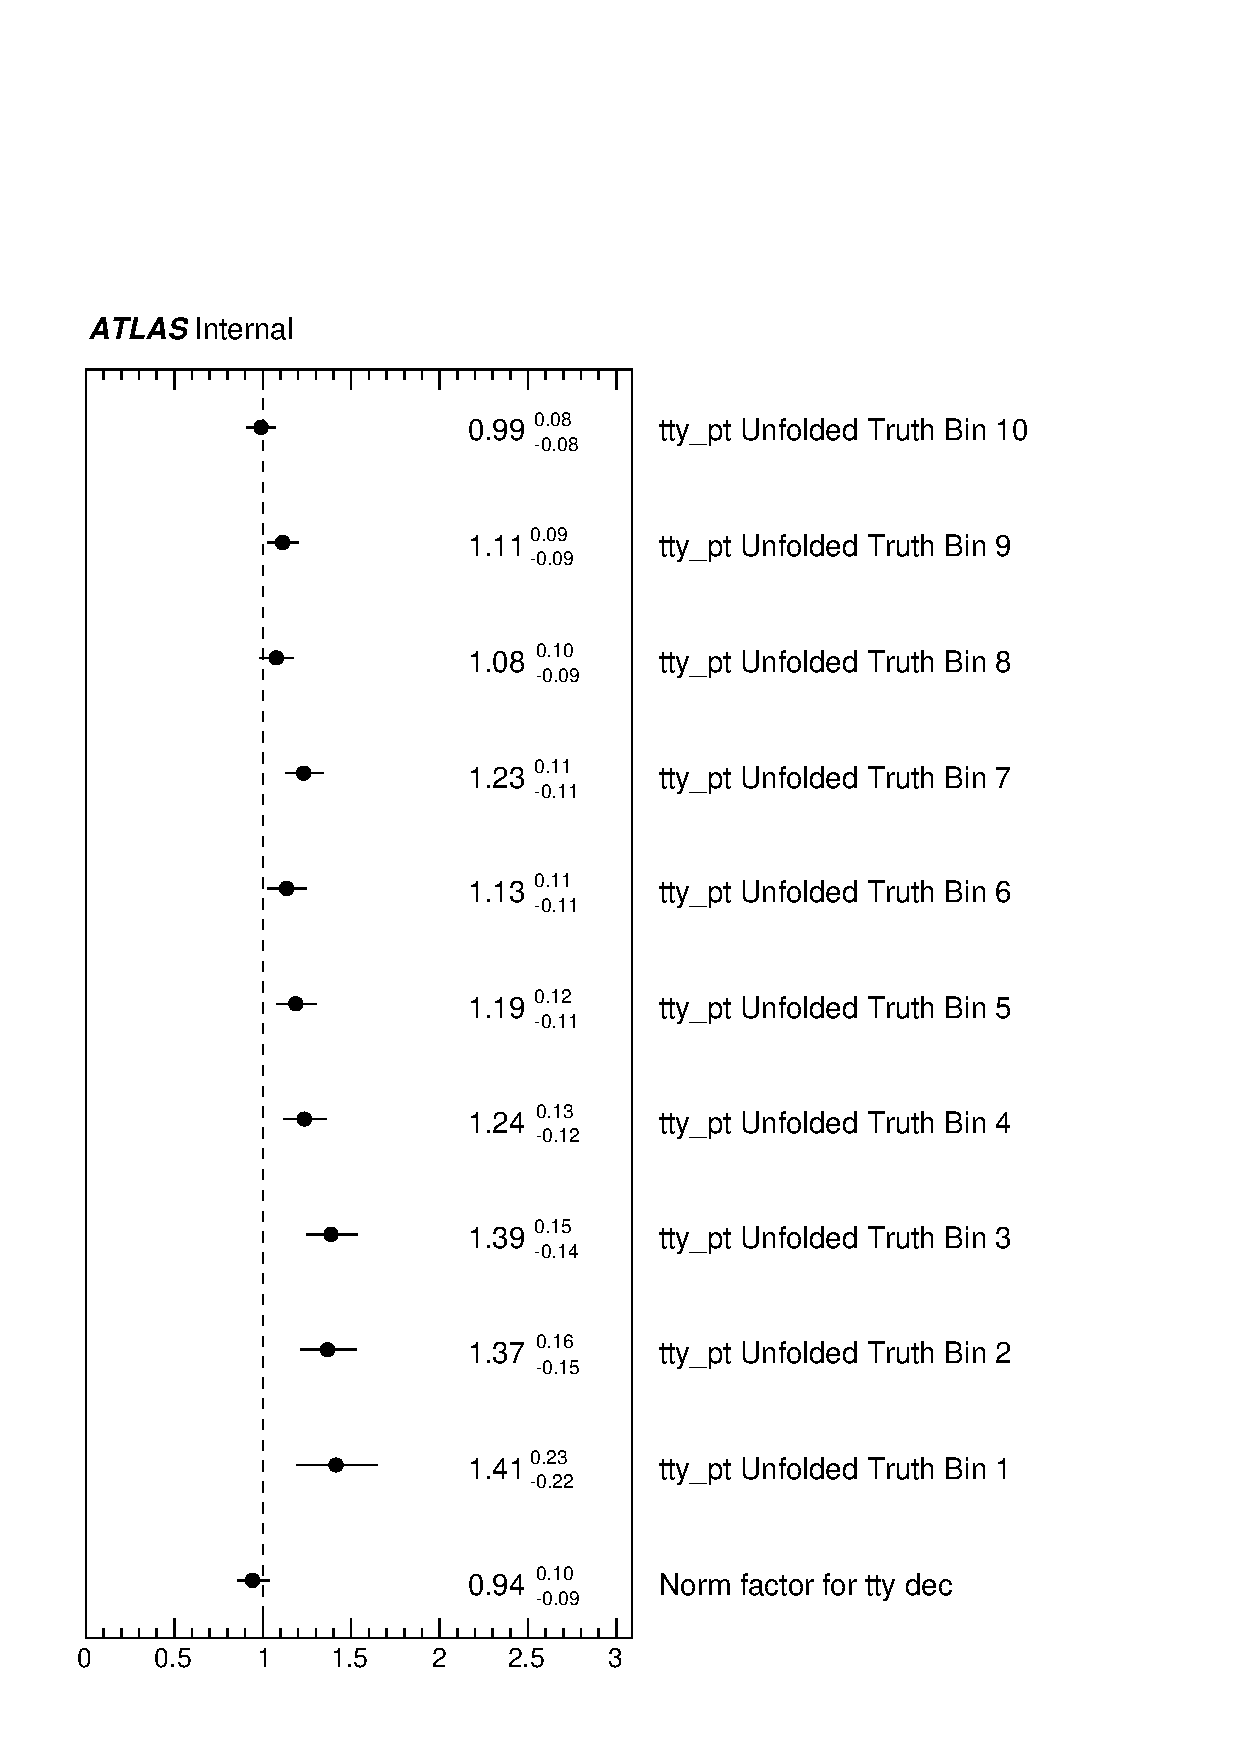
\includegraphics[width=0.3\textwidth]{figures/diff_xsec/ljet_tty_prod_mu_blinded/Unfolded_data/tty1l_pt_all_syst/NormFactors.pdf}}
  \quad
  \subfloat[]{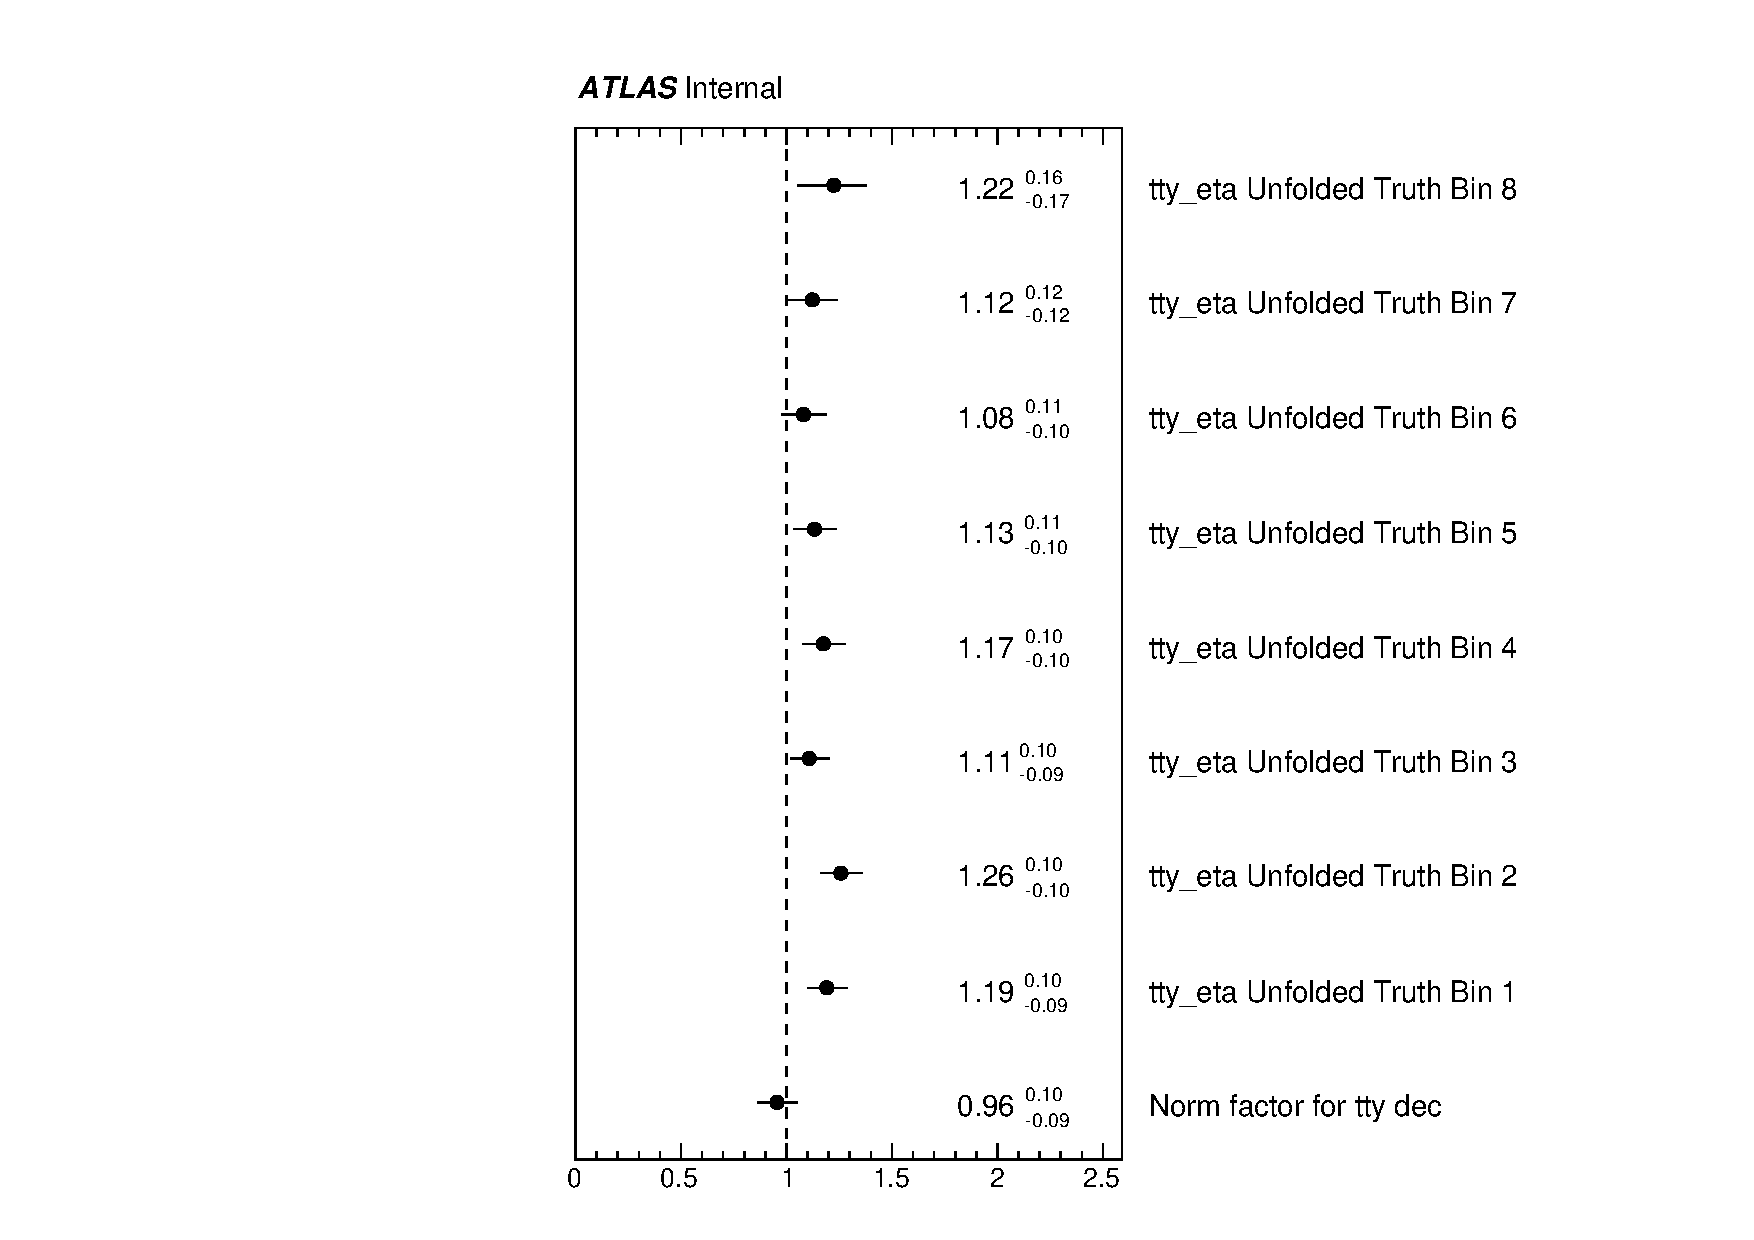
\includegraphics[width=0.3\textwidth]{figures/diff_xsec/ljet_tty_prod_mu_blinded/Unfolded_data/tty1l_eta_all_syst/NormFactors.pdf}}
  \quad
  \subfloat[]{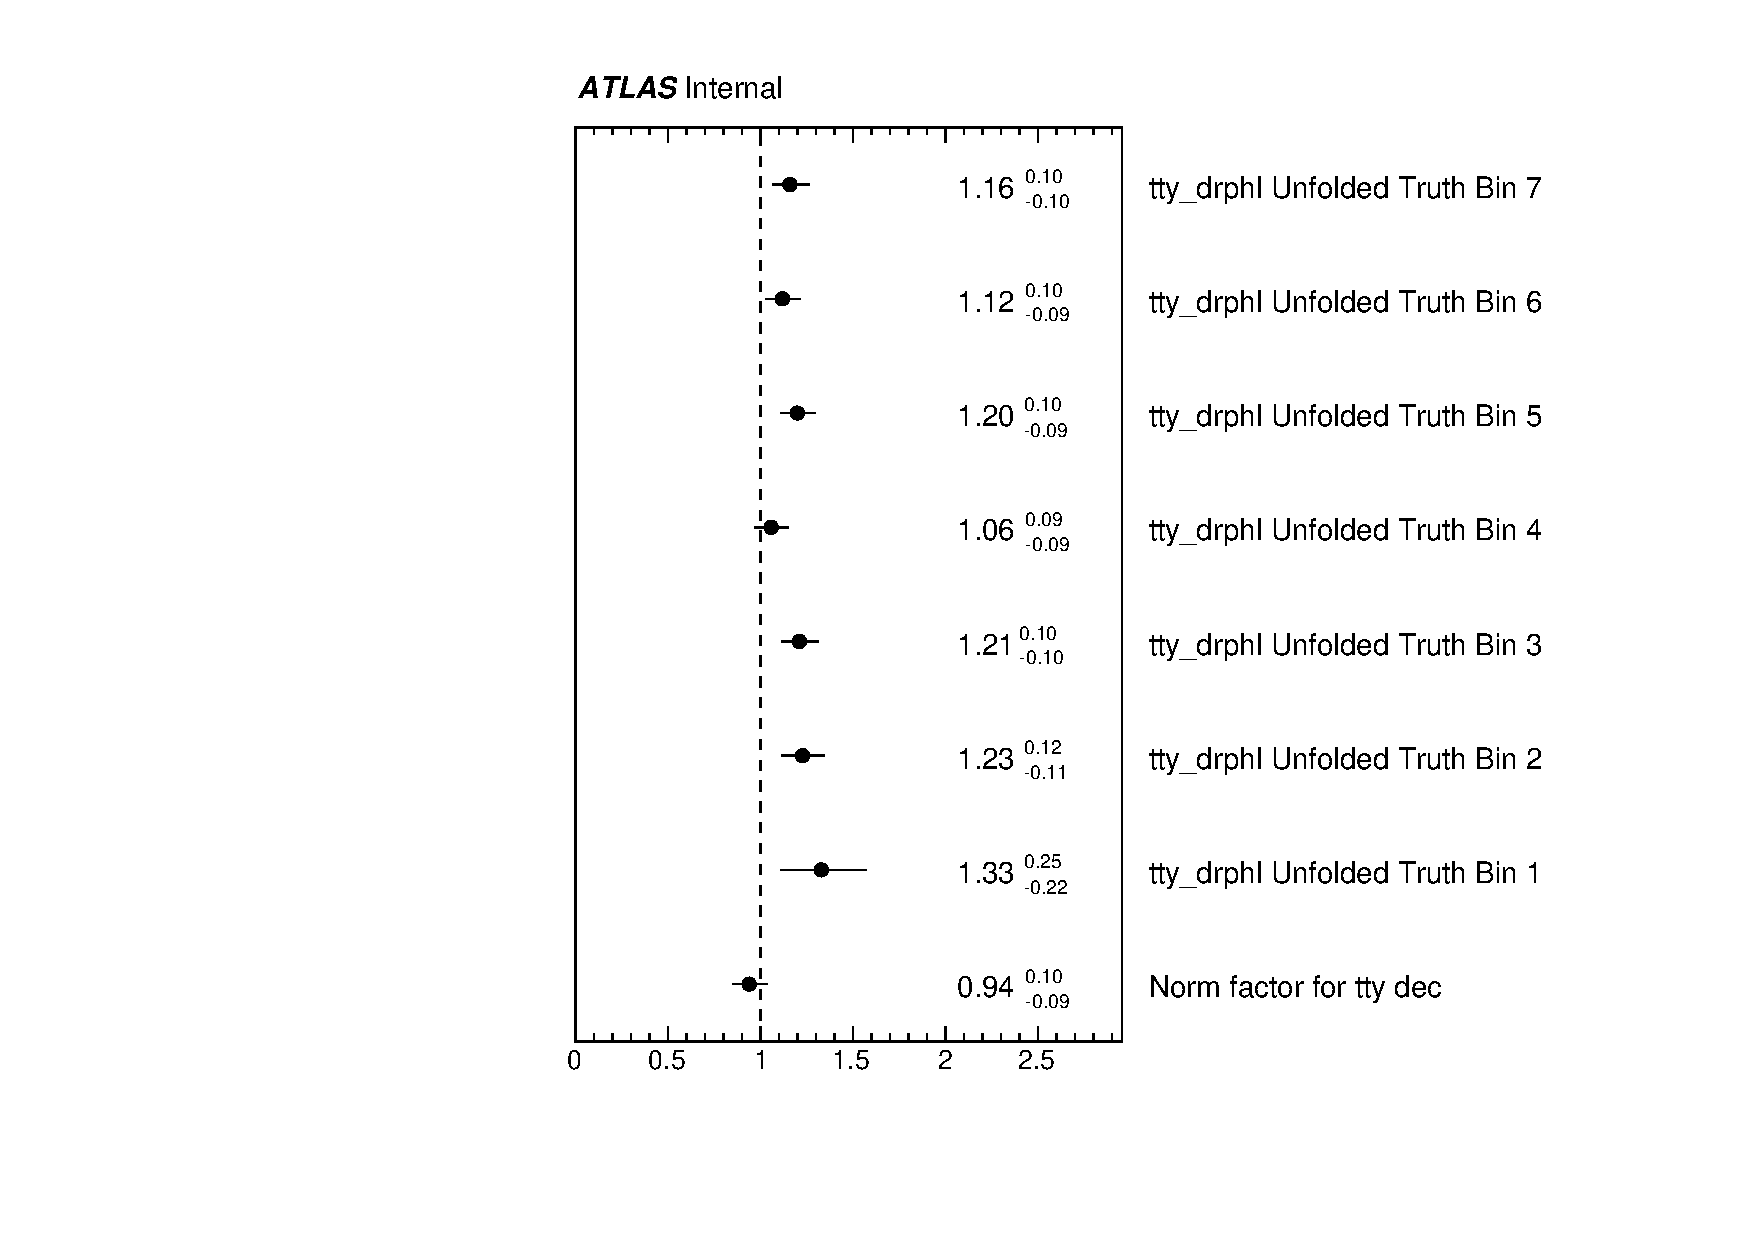
\includegraphics[width=0.3\textwidth]{figures/diff_xsec/ljet_tty_prod_mu_blinded/Unfolded_data/tty1l_dr_all_syst/NormFactors.pdf}}
  \quad
  \subfloat[]{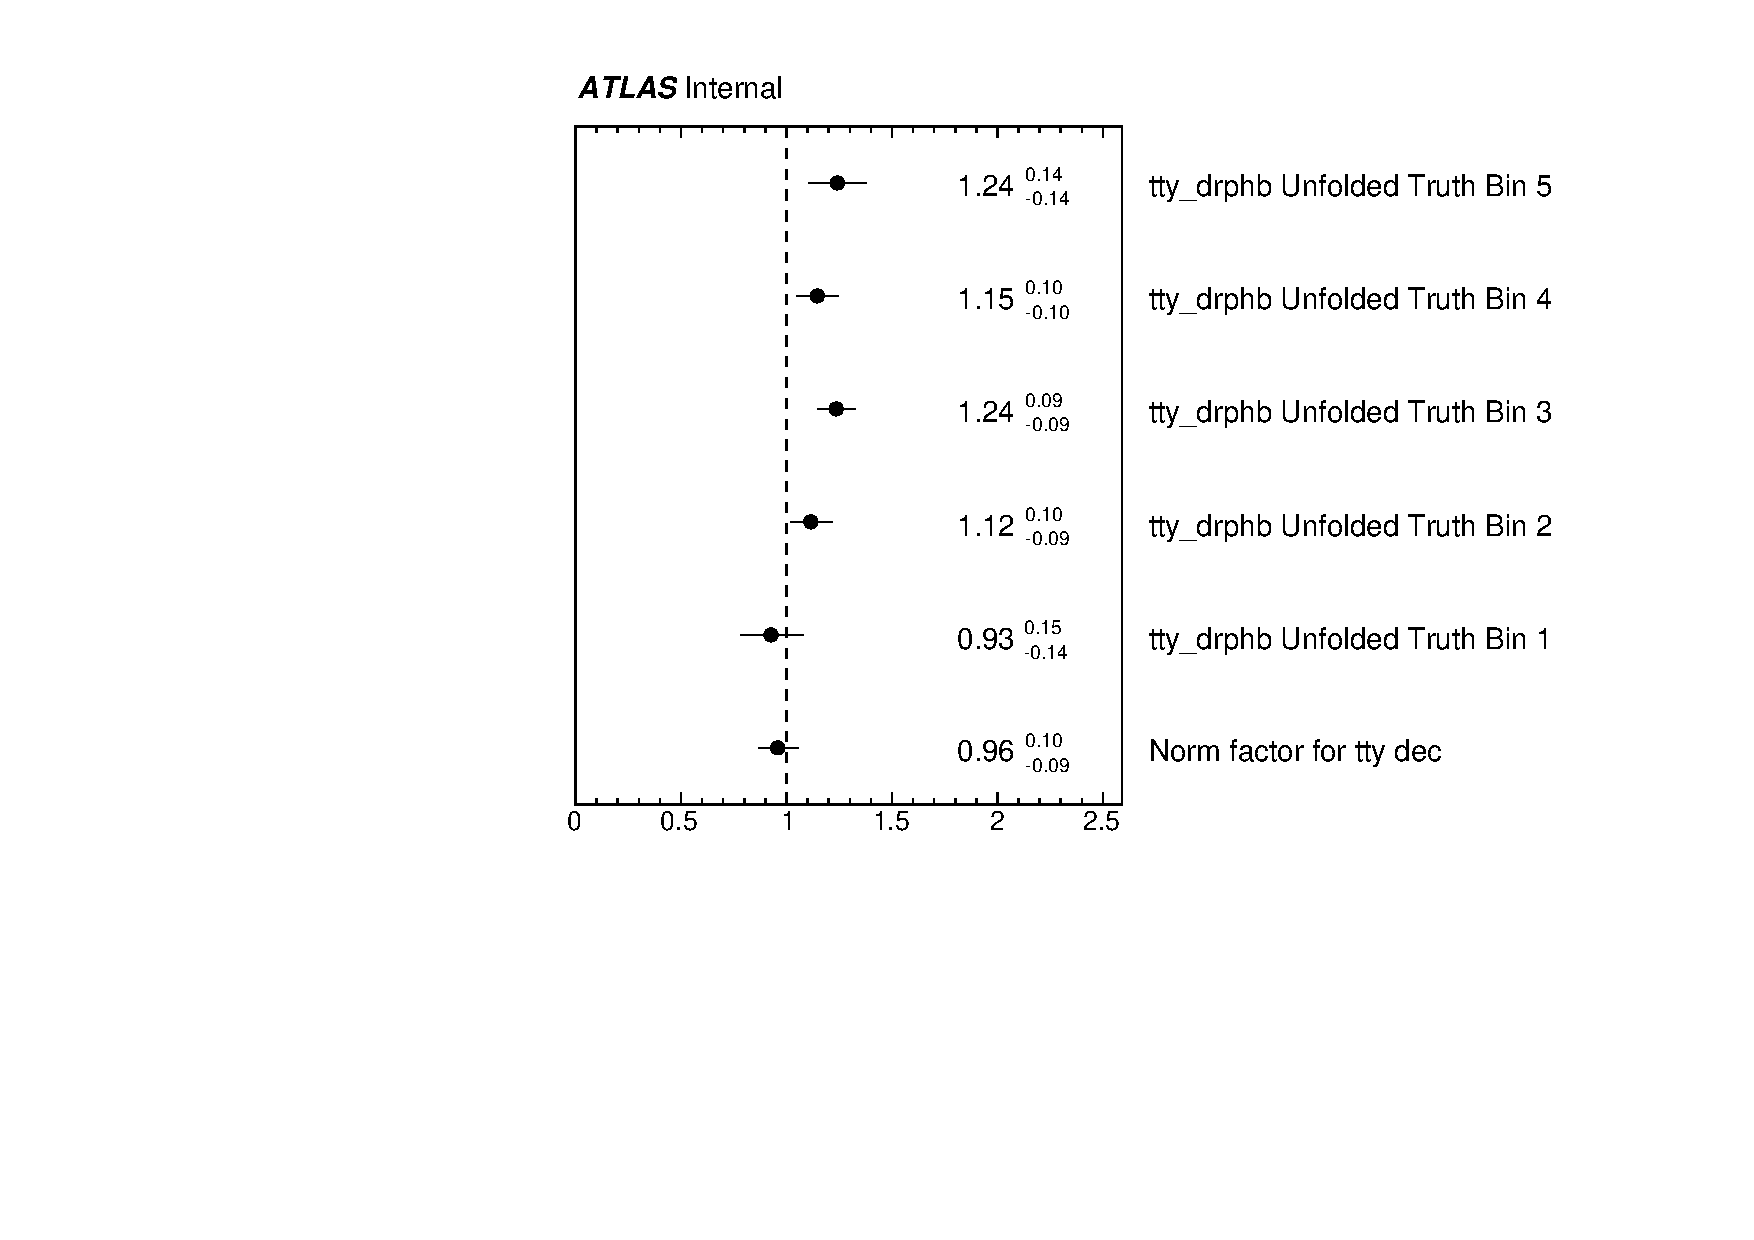
\includegraphics[width=0.3\textwidth]{figures/diff_xsec/ljet_tty_prod_mu_blinded/Unfolded_data/tty1l_drphb_all_syst/NormFactors.pdf}}
  \quad
  \subfloat[]{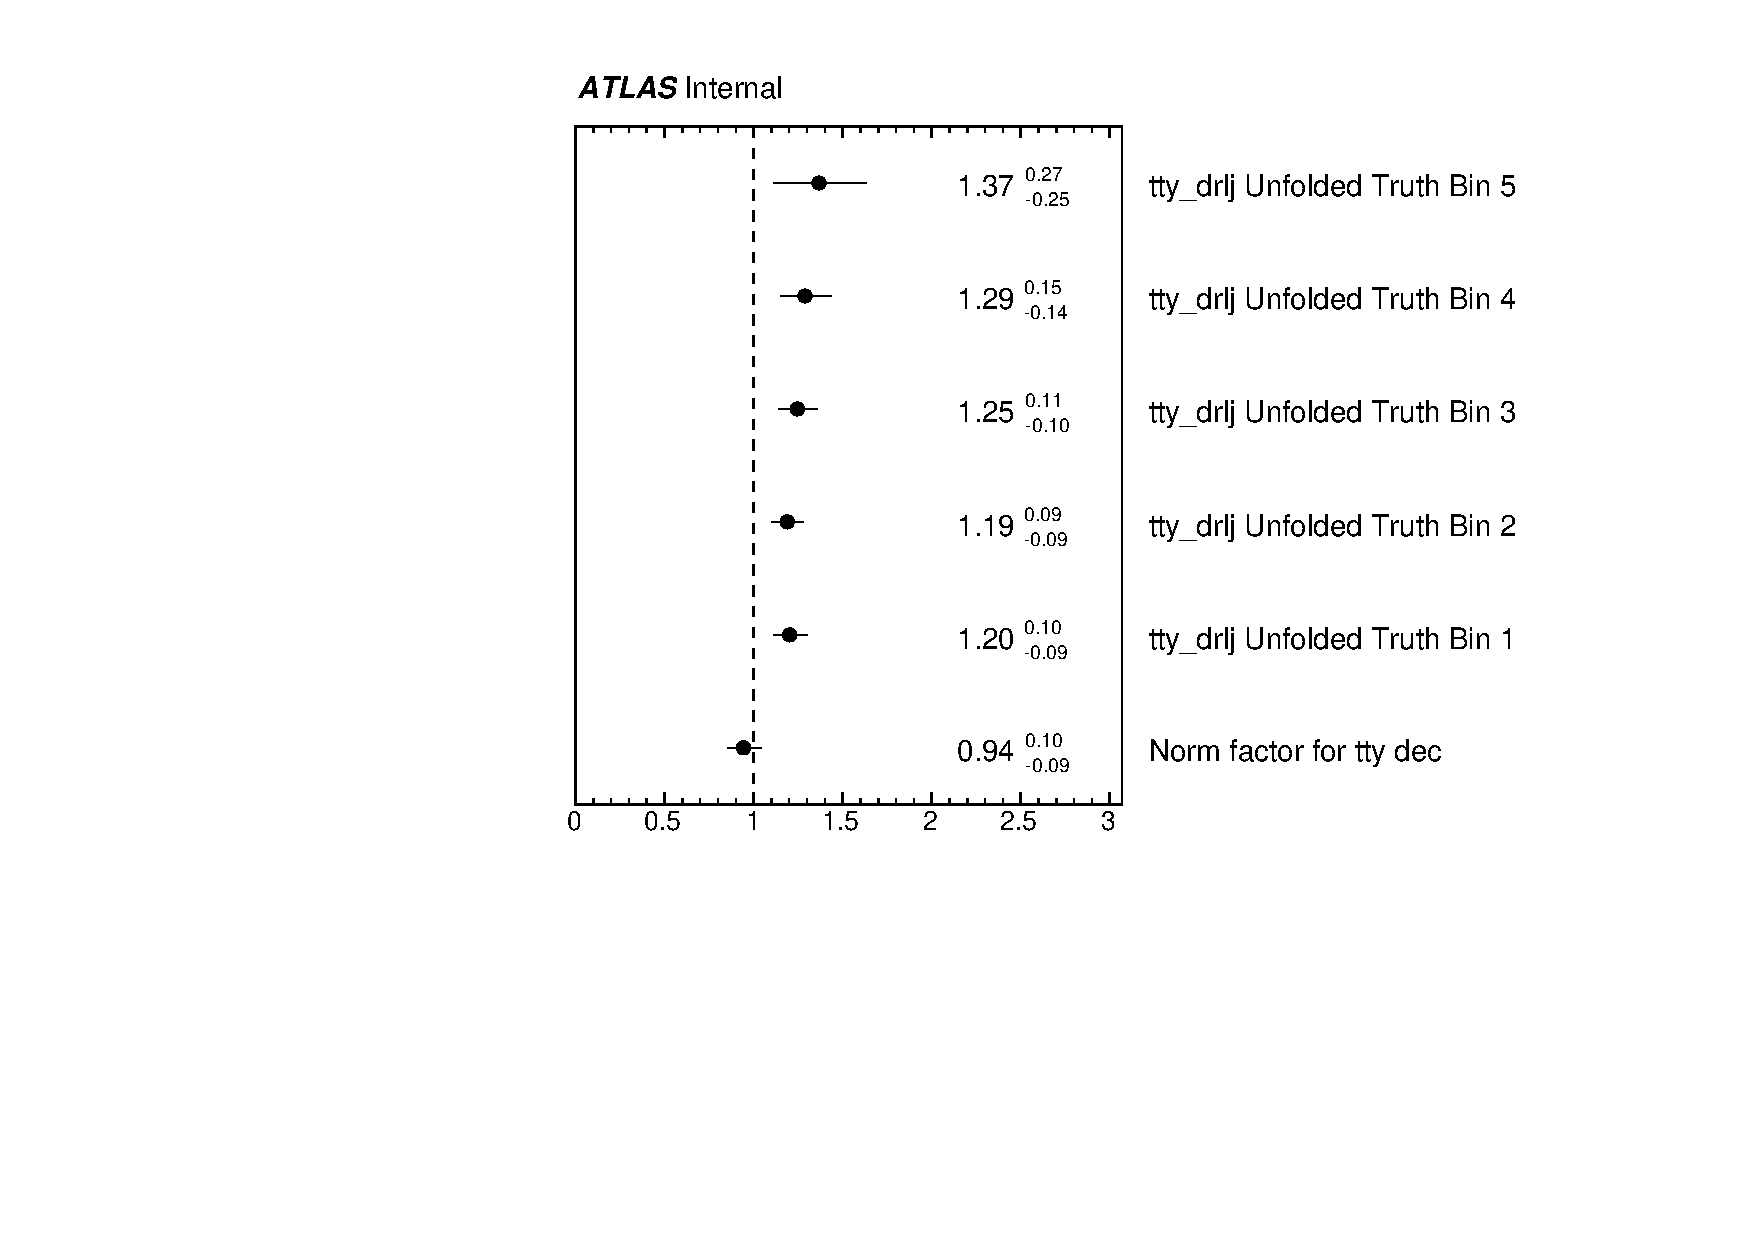
\includegraphics[width=0.3\textwidth]{figures/diff_xsec/ljet_tty_prod_mu_blinded/Unfolded_data/tty1l_drlj_all_syst/NormFactors.pdf}}
  \quad
  \subfloat[]{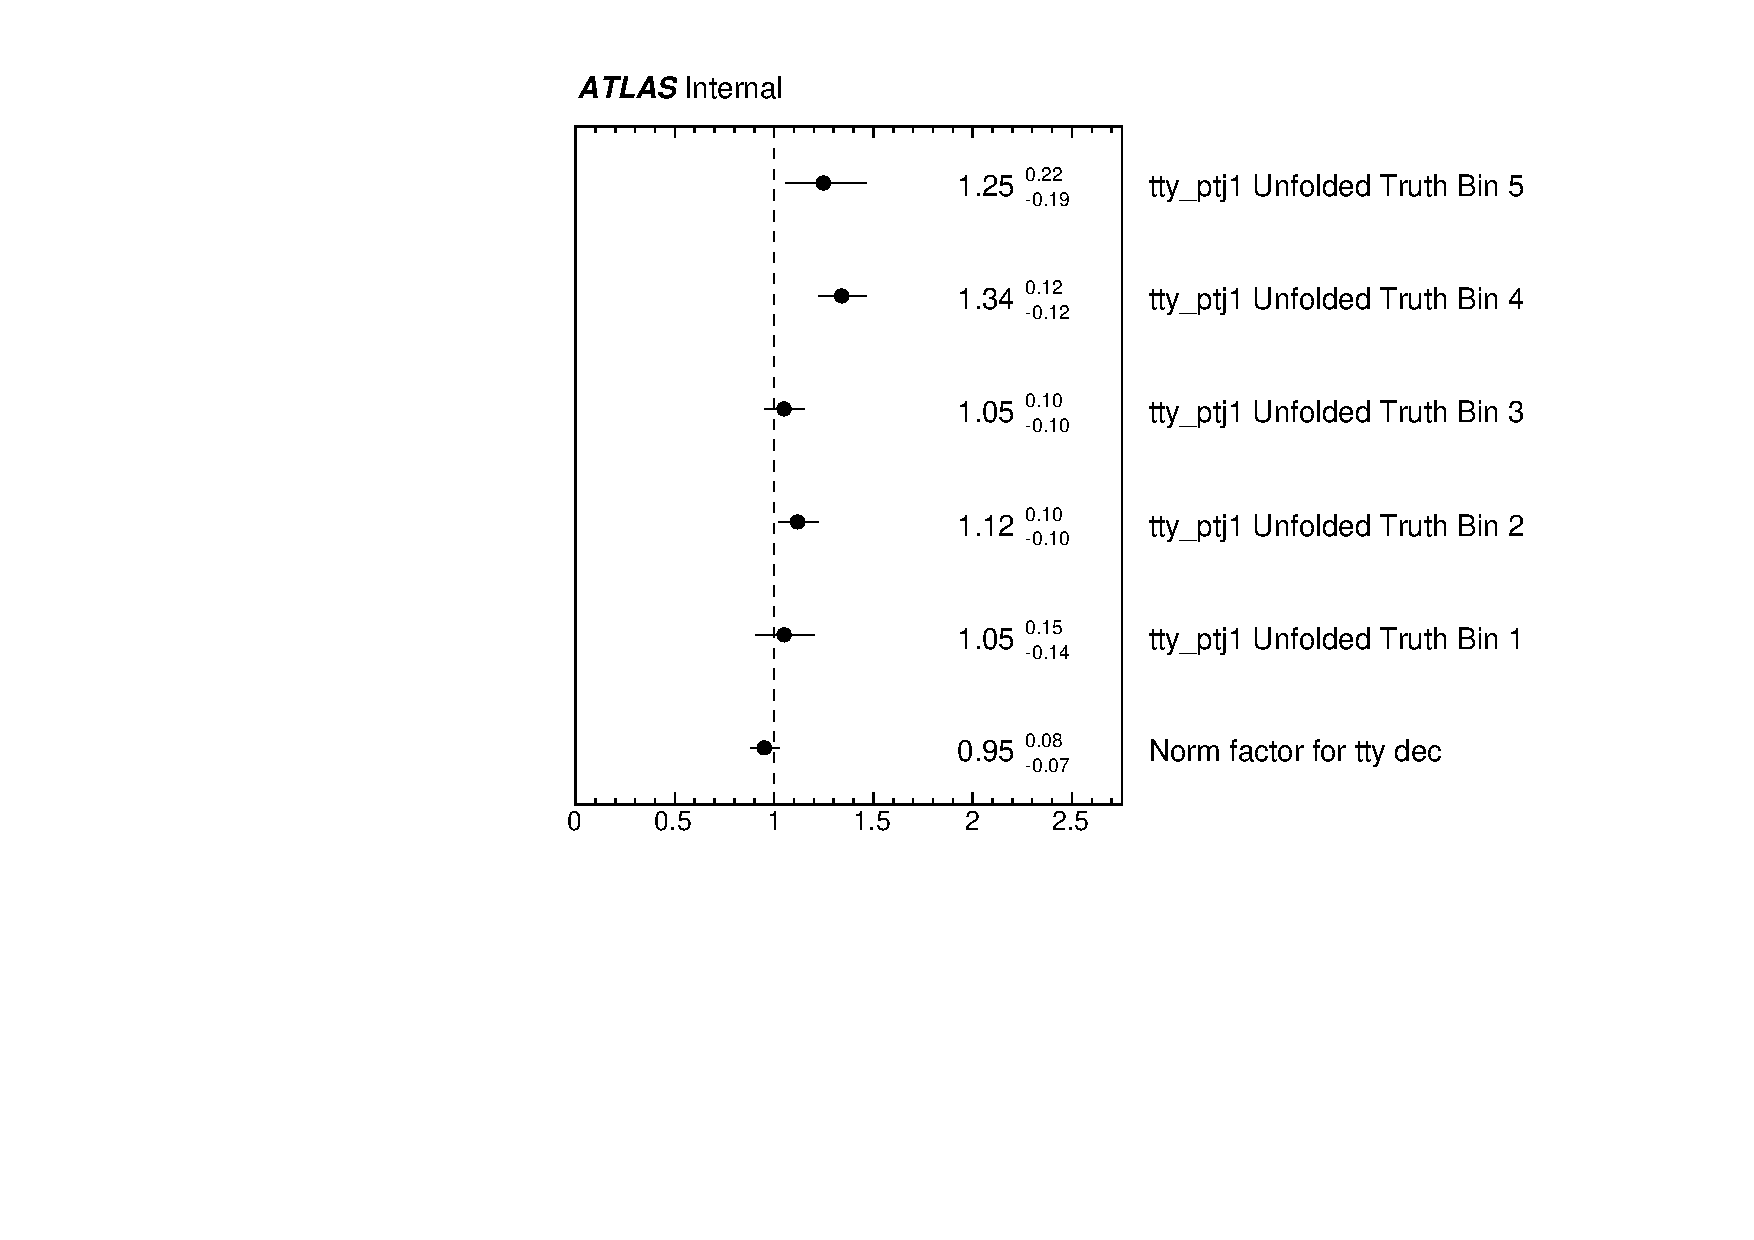
\includegraphics[width=0.3\textwidth]{figures/diff_xsec/ljet_tty_prod_mu_blinded/Unfolded_data/tty1l_ptj1_all_syst/NormFactors.pdf}}
  \caption{ The figure displays the normalization factors obtained from the fit for \tty production measurement in single-lepton channel for the following observables: (a) $p_T(\gamma)$, (b) $|\eta(\gamma|)$, (c) $\Delta R_{min}(\gamma, l)$, (d) $\Delta R(\gamma, b)$, (e) $\Delta R_{min}(l, j)$, (f) $p_T(j1)$.}
  \label{fig:pt_unfolded_ljet_table_realdata}
\end{figure}
\FloatBarrier


\begin{figure}[ht]
  \centering
  \subfloat[]{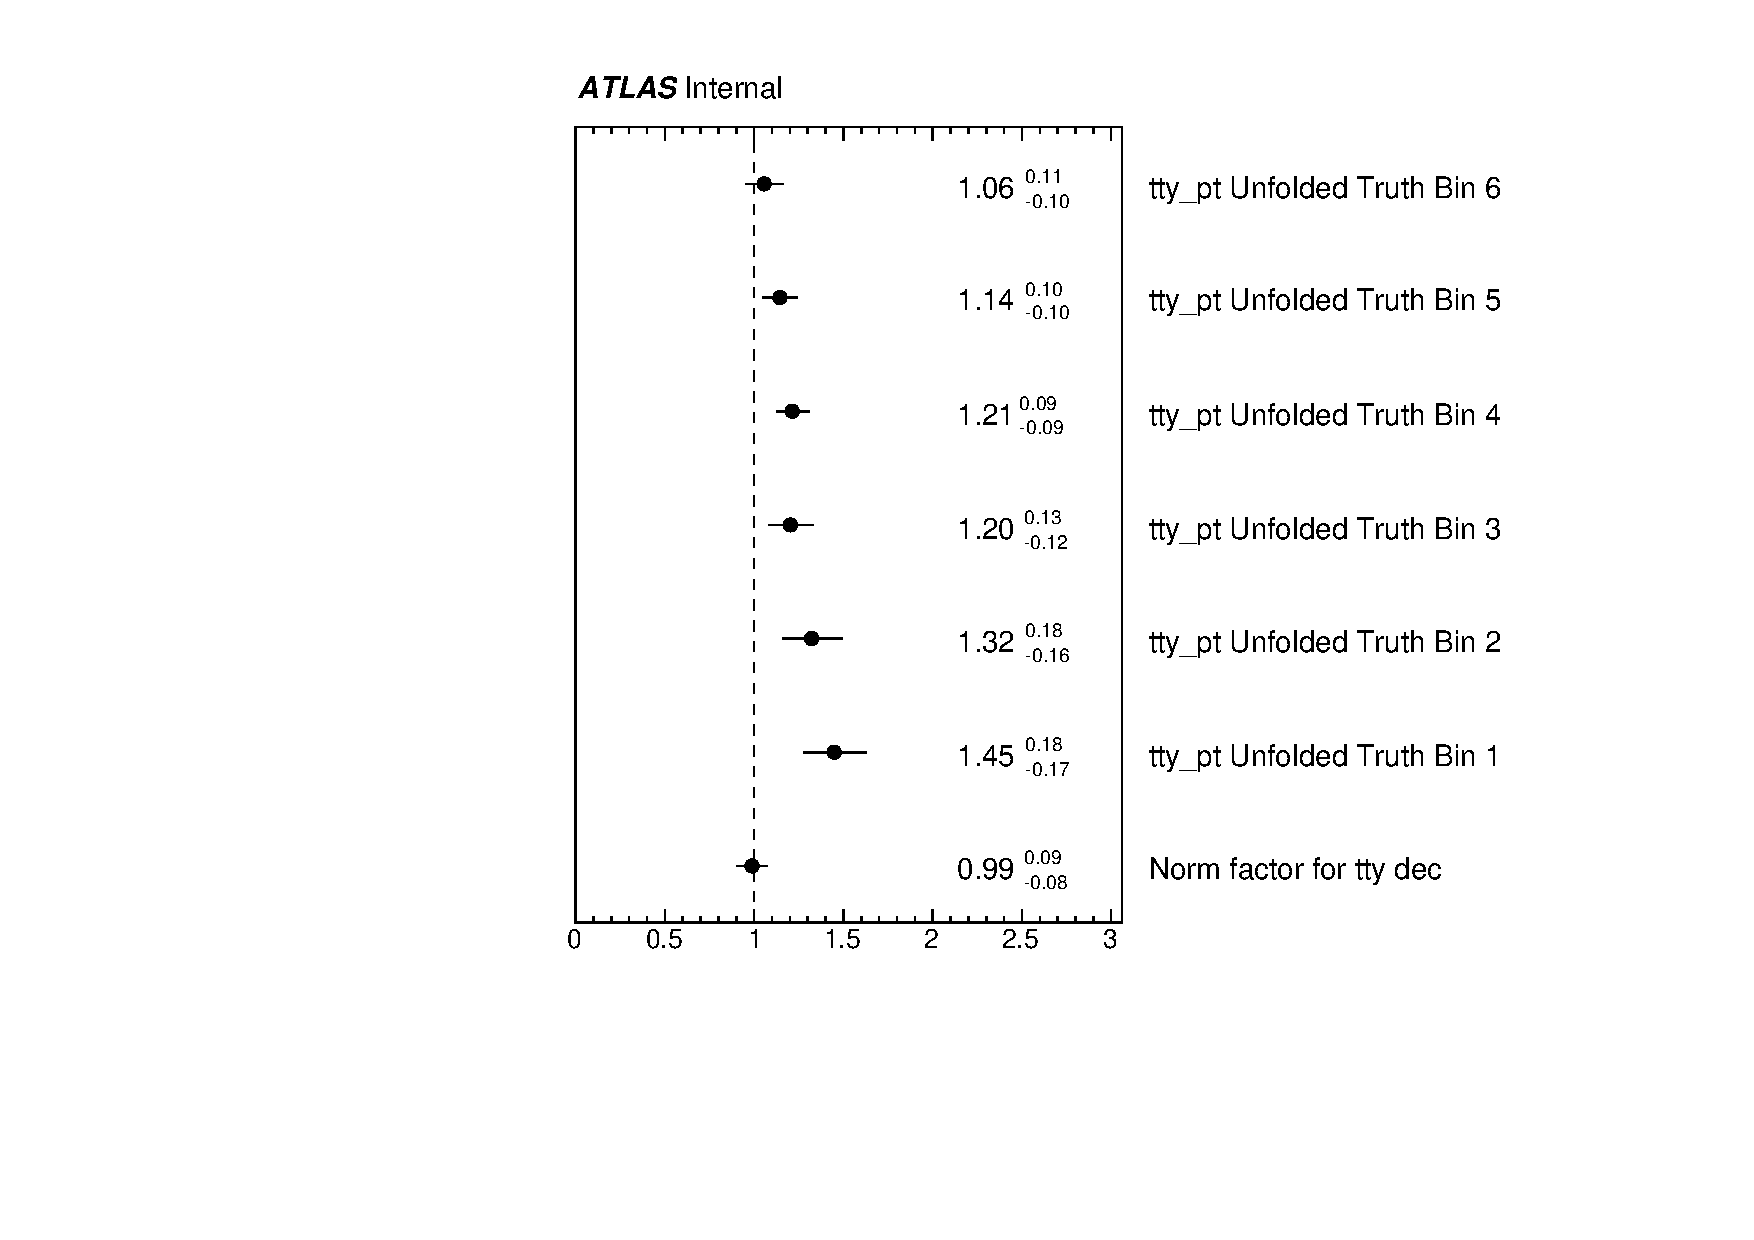
\includegraphics[width=0.3\textwidth]{figures/diff_xsec/dilep_tty_prod_mu_blinded/Unfolded_data/tty2l_pt_all_syst/NormFactors.pdf}}
  \quad
  \subfloat[]{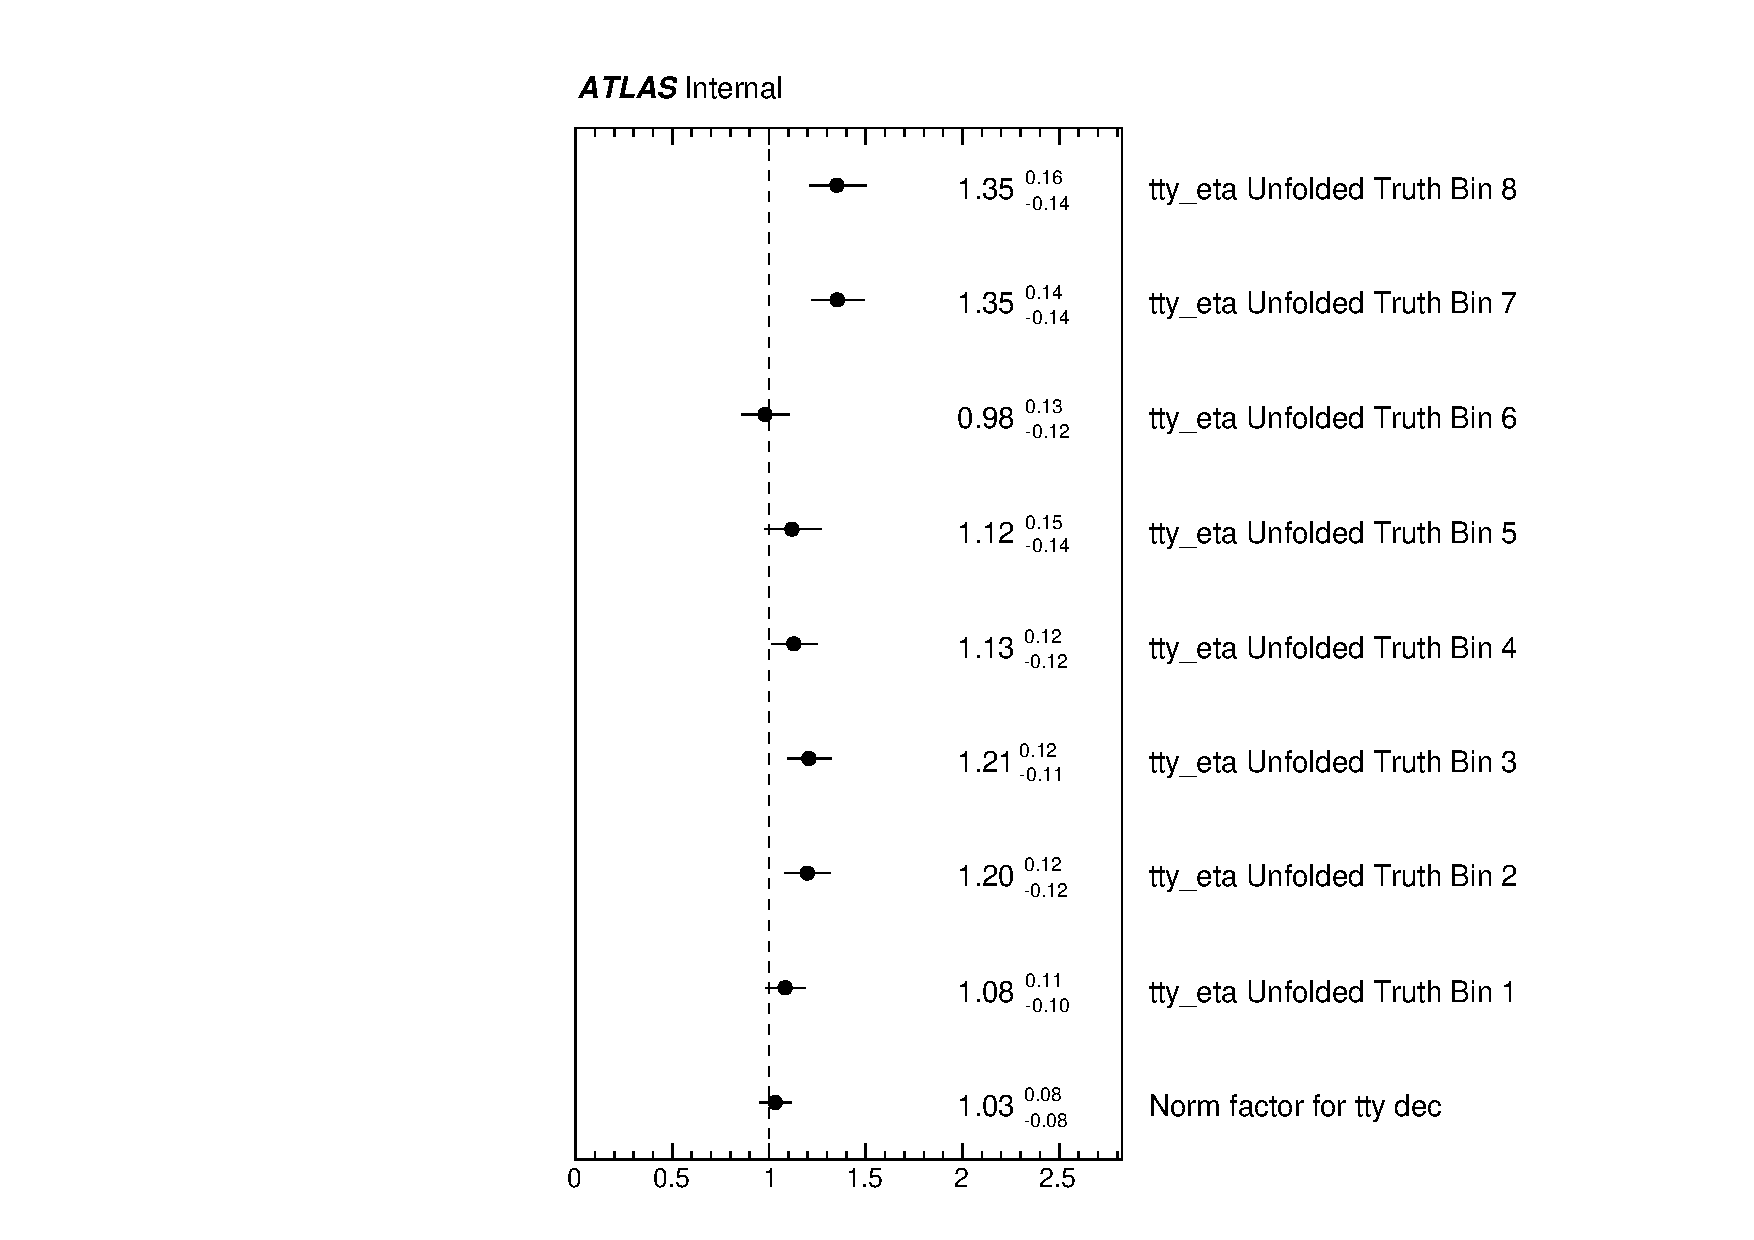
\includegraphics[width=0.3\textwidth]{figures/diff_xsec/dilep_tty_prod_mu_blinded/Unfolded_data/tty2l_eta_all_syst/NormFactors.pdf}}
  \quad
  \subfloat[]{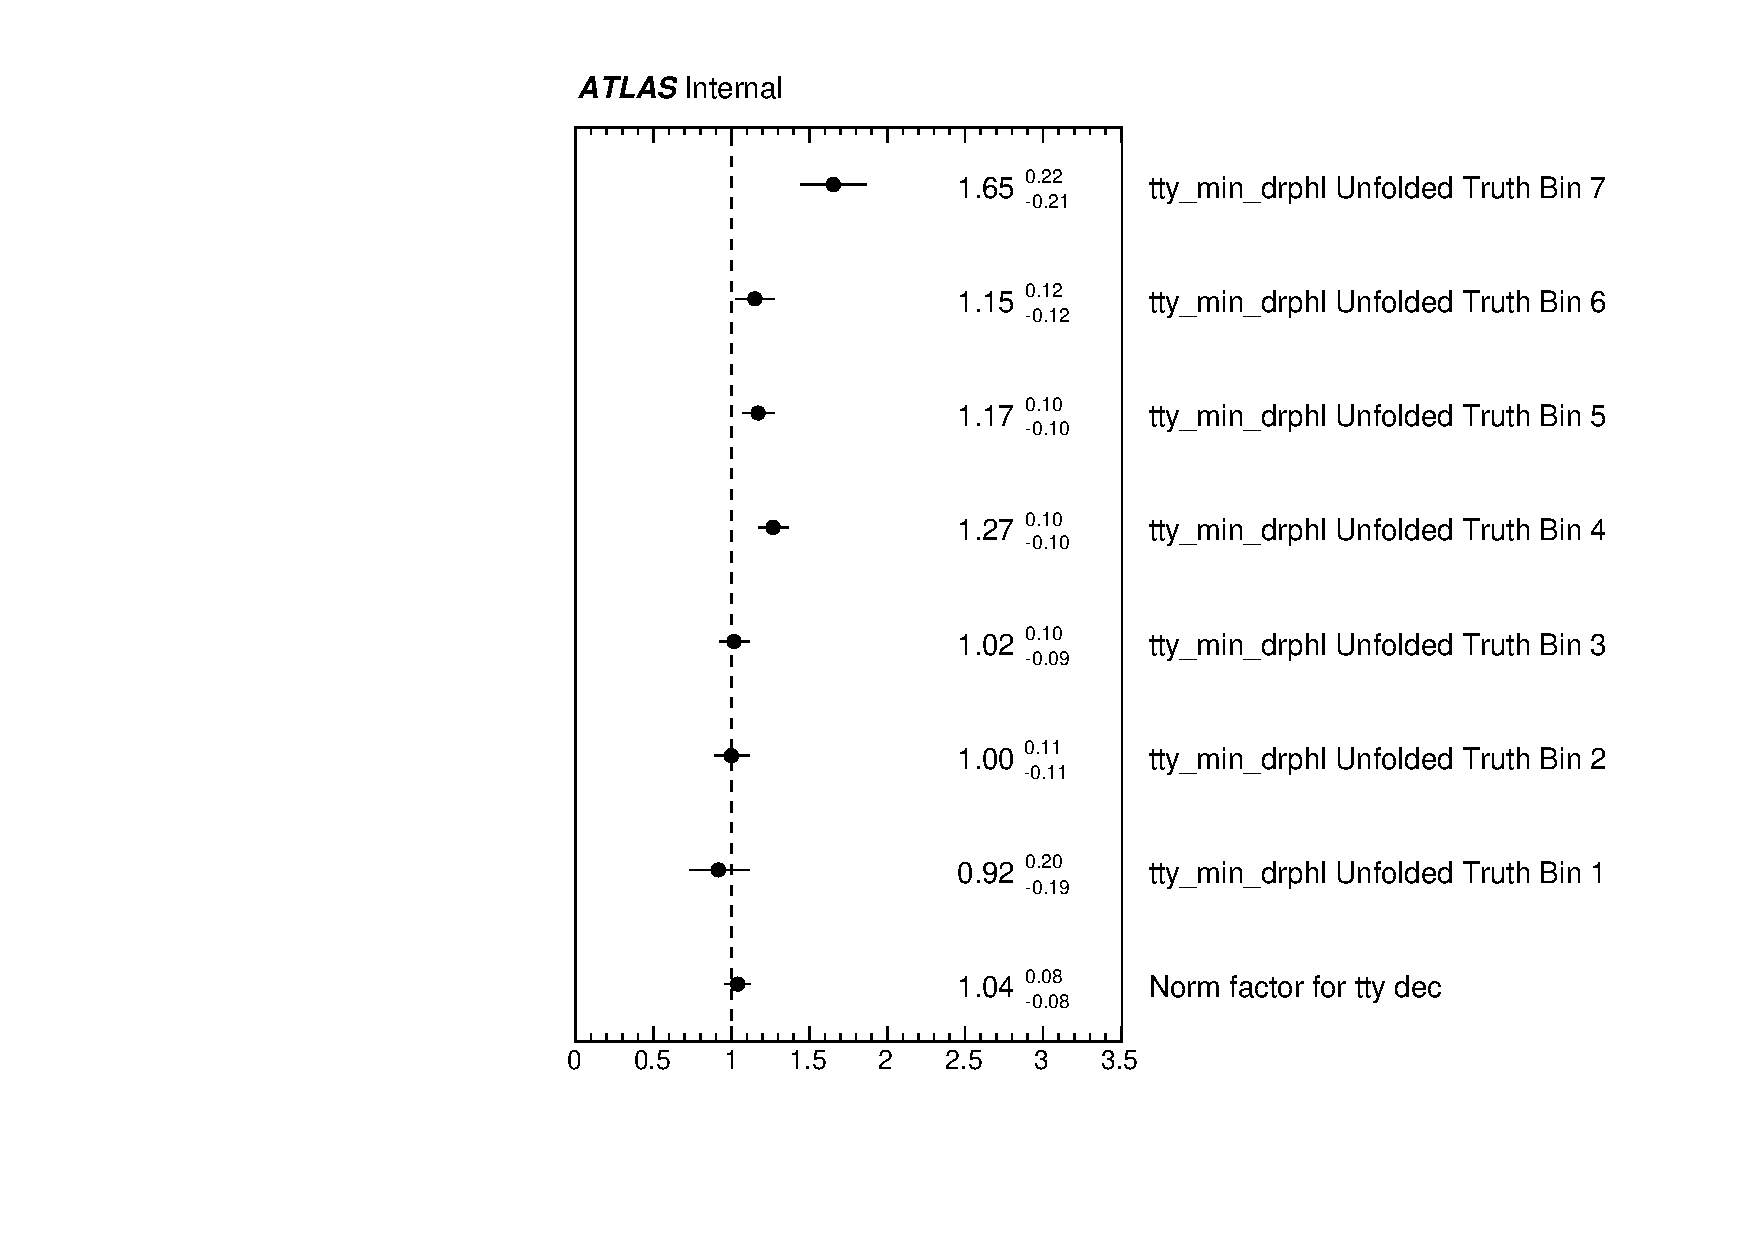
\includegraphics[width=0.3\textwidth]{figures/diff_xsec/dilep_tty_prod_mu_blinded/Unfolded_data/tty2l_dr_all_syst/NormFactors.pdf}}
  \quad
  \subfloat[]{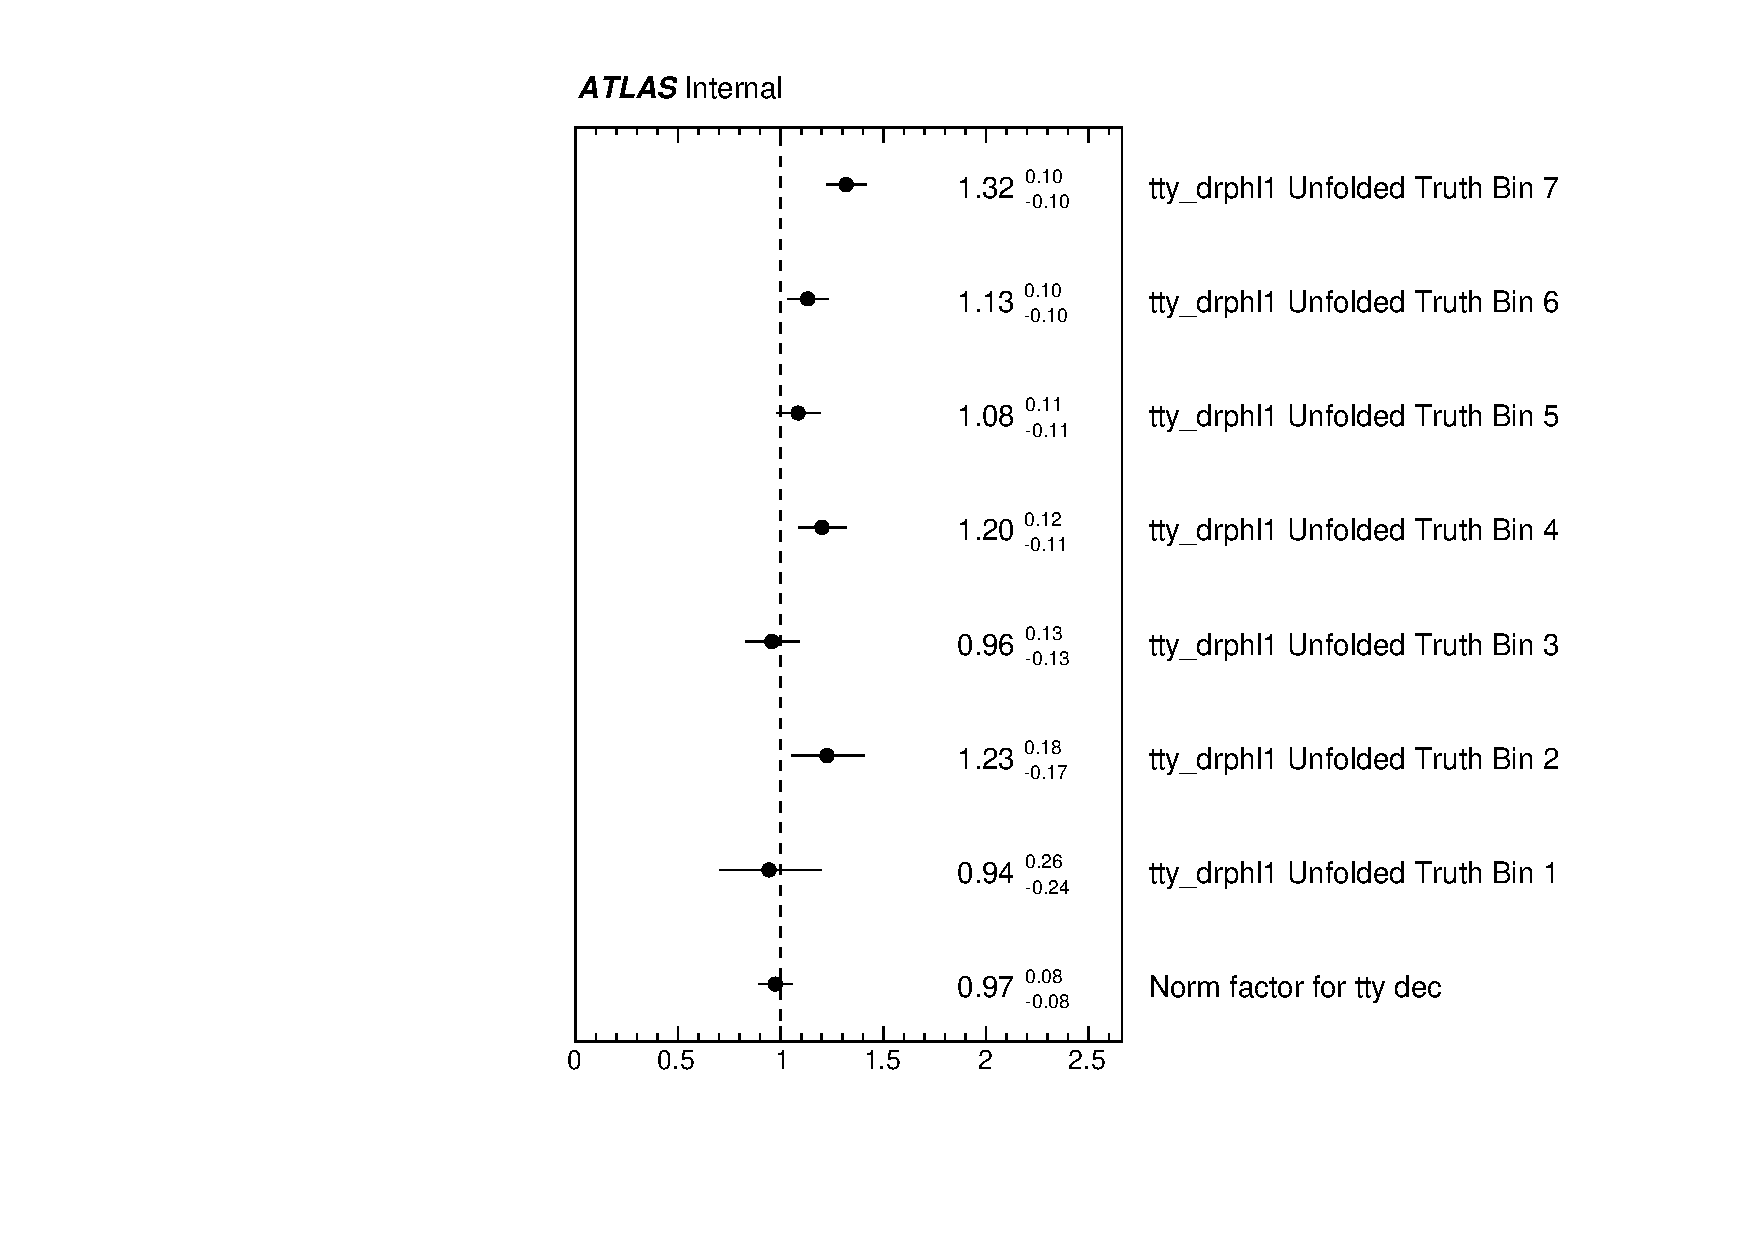
\includegraphics[width=0.3\textwidth]{figures/diff_xsec/dilep_tty_prod_mu_blinded/Unfolded_data/tty2l_dr1_all_syst/NormFactors.pdf}}
  \quad
  \subfloat[]{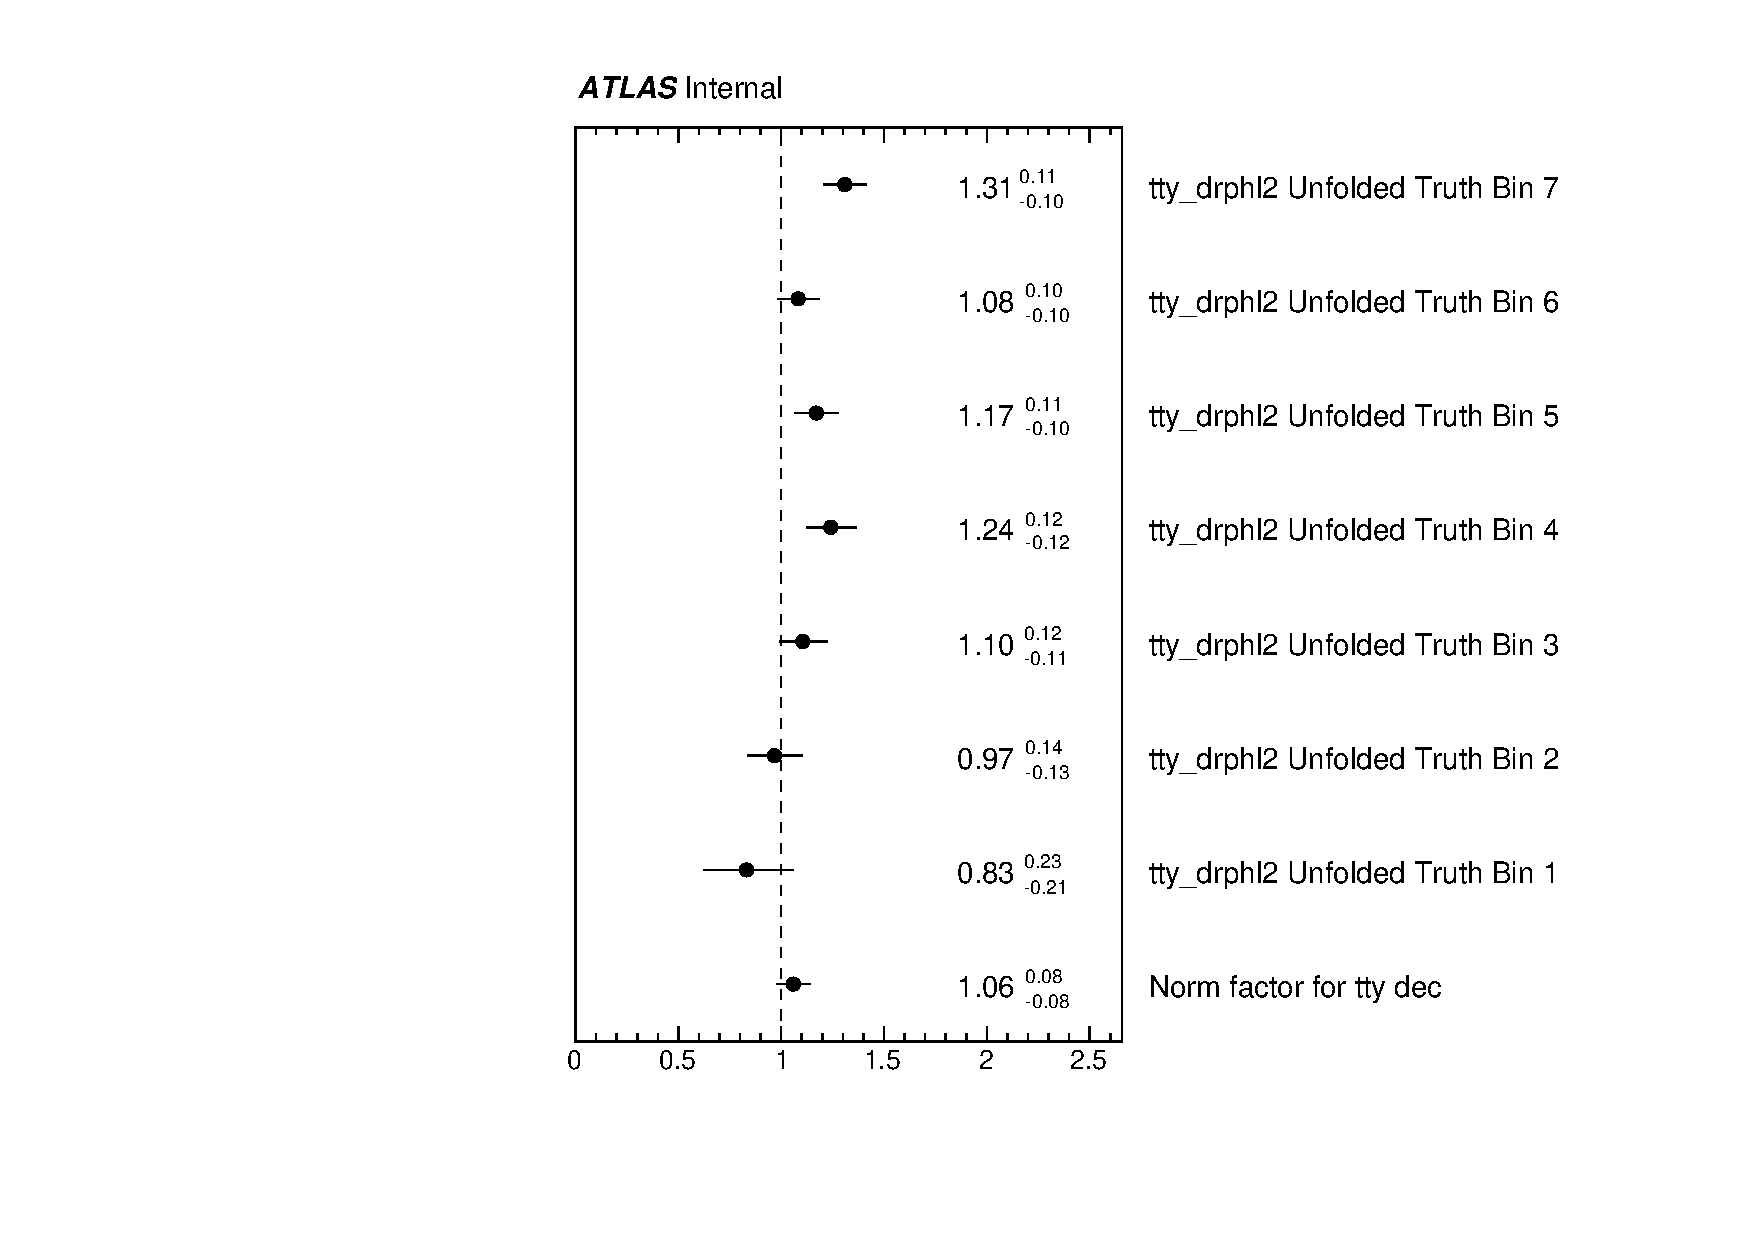
\includegraphics[width=0.3\textwidth]{figures/diff_xsec/dilep_tty_prod_mu_blinded/Unfolded_data/tty2l_dr2_all_syst/NormFactors.pdf}}
  \quad
  \subfloat[]{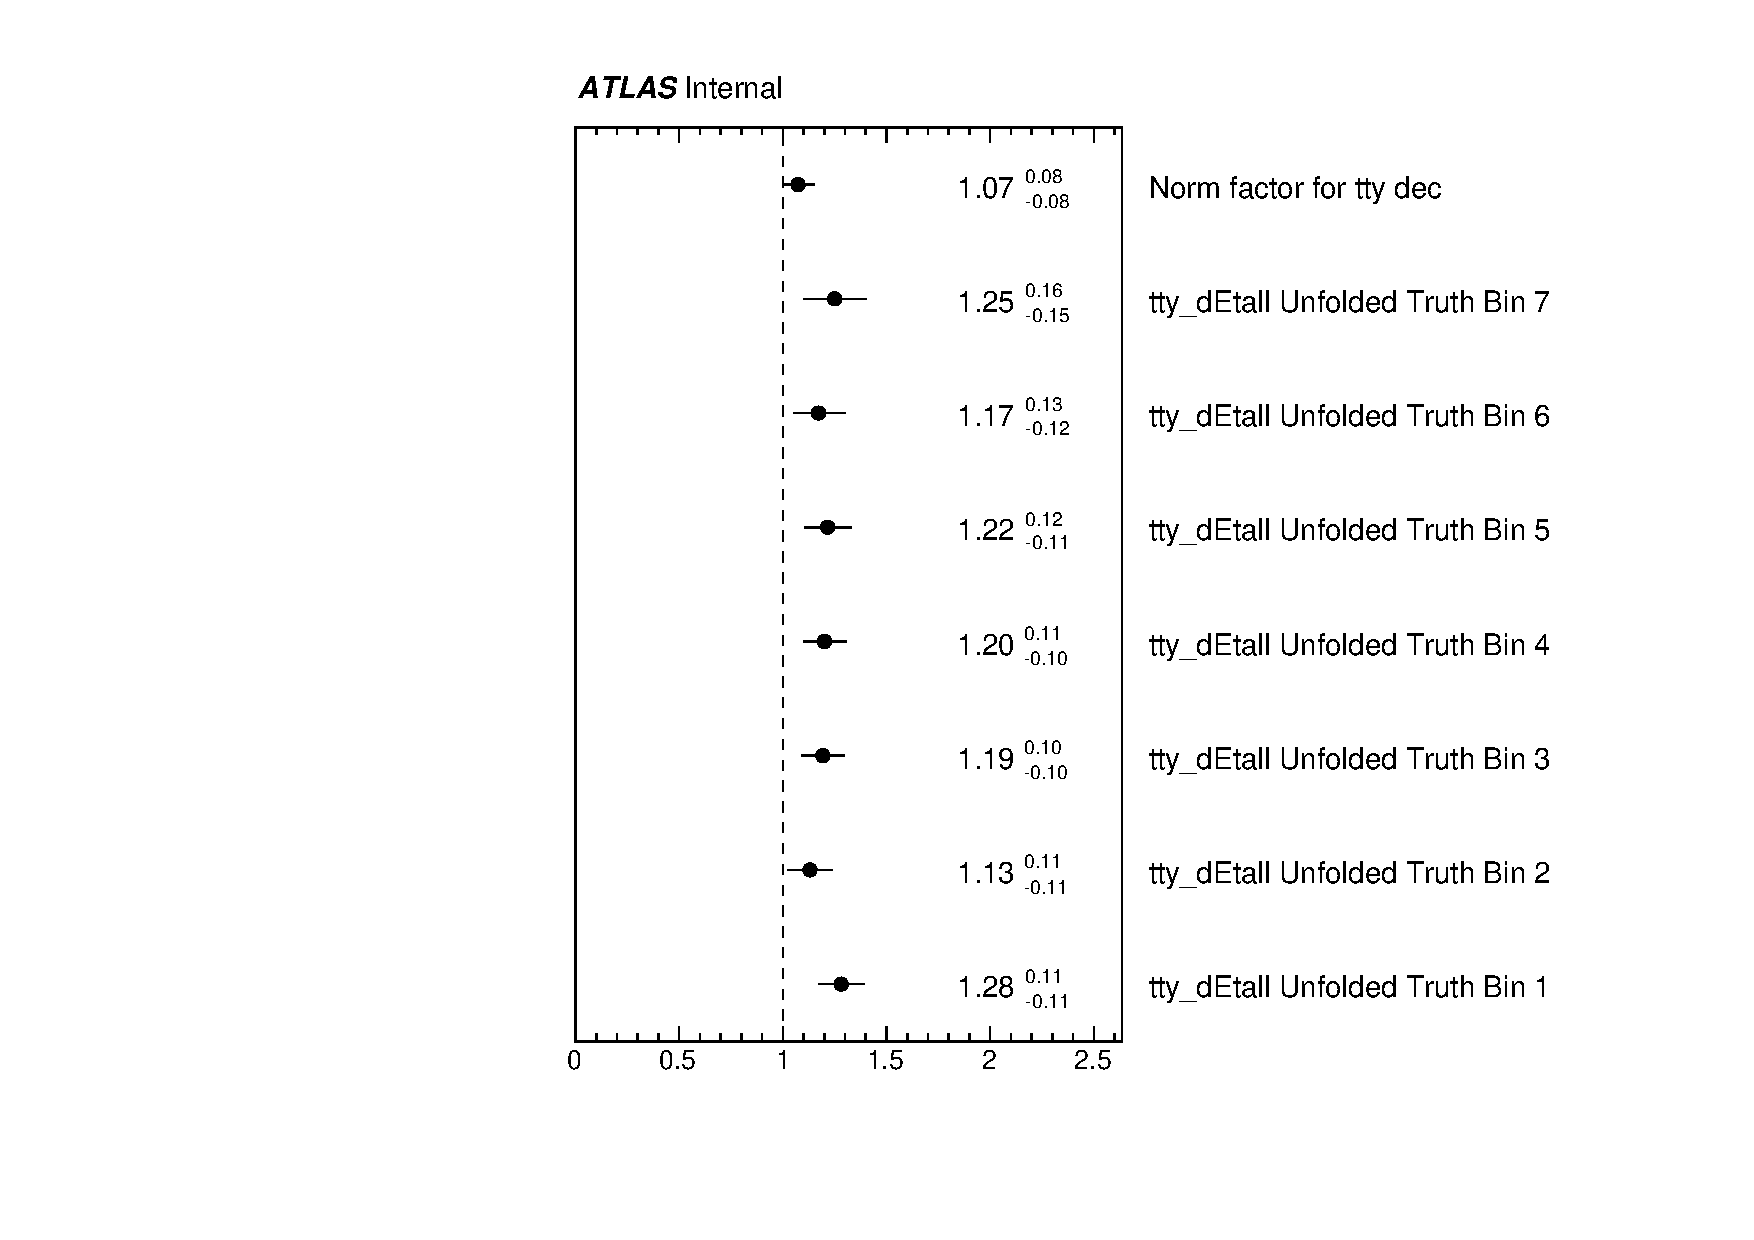
\includegraphics[width=0.3\textwidth]{figures/diff_xsec/dilep_tty_prod_mu_blinded/Unfolded_data/tty2l_dEtall_all_syst/NormFactors.pdf}}
  \quad
  \subfloat[]{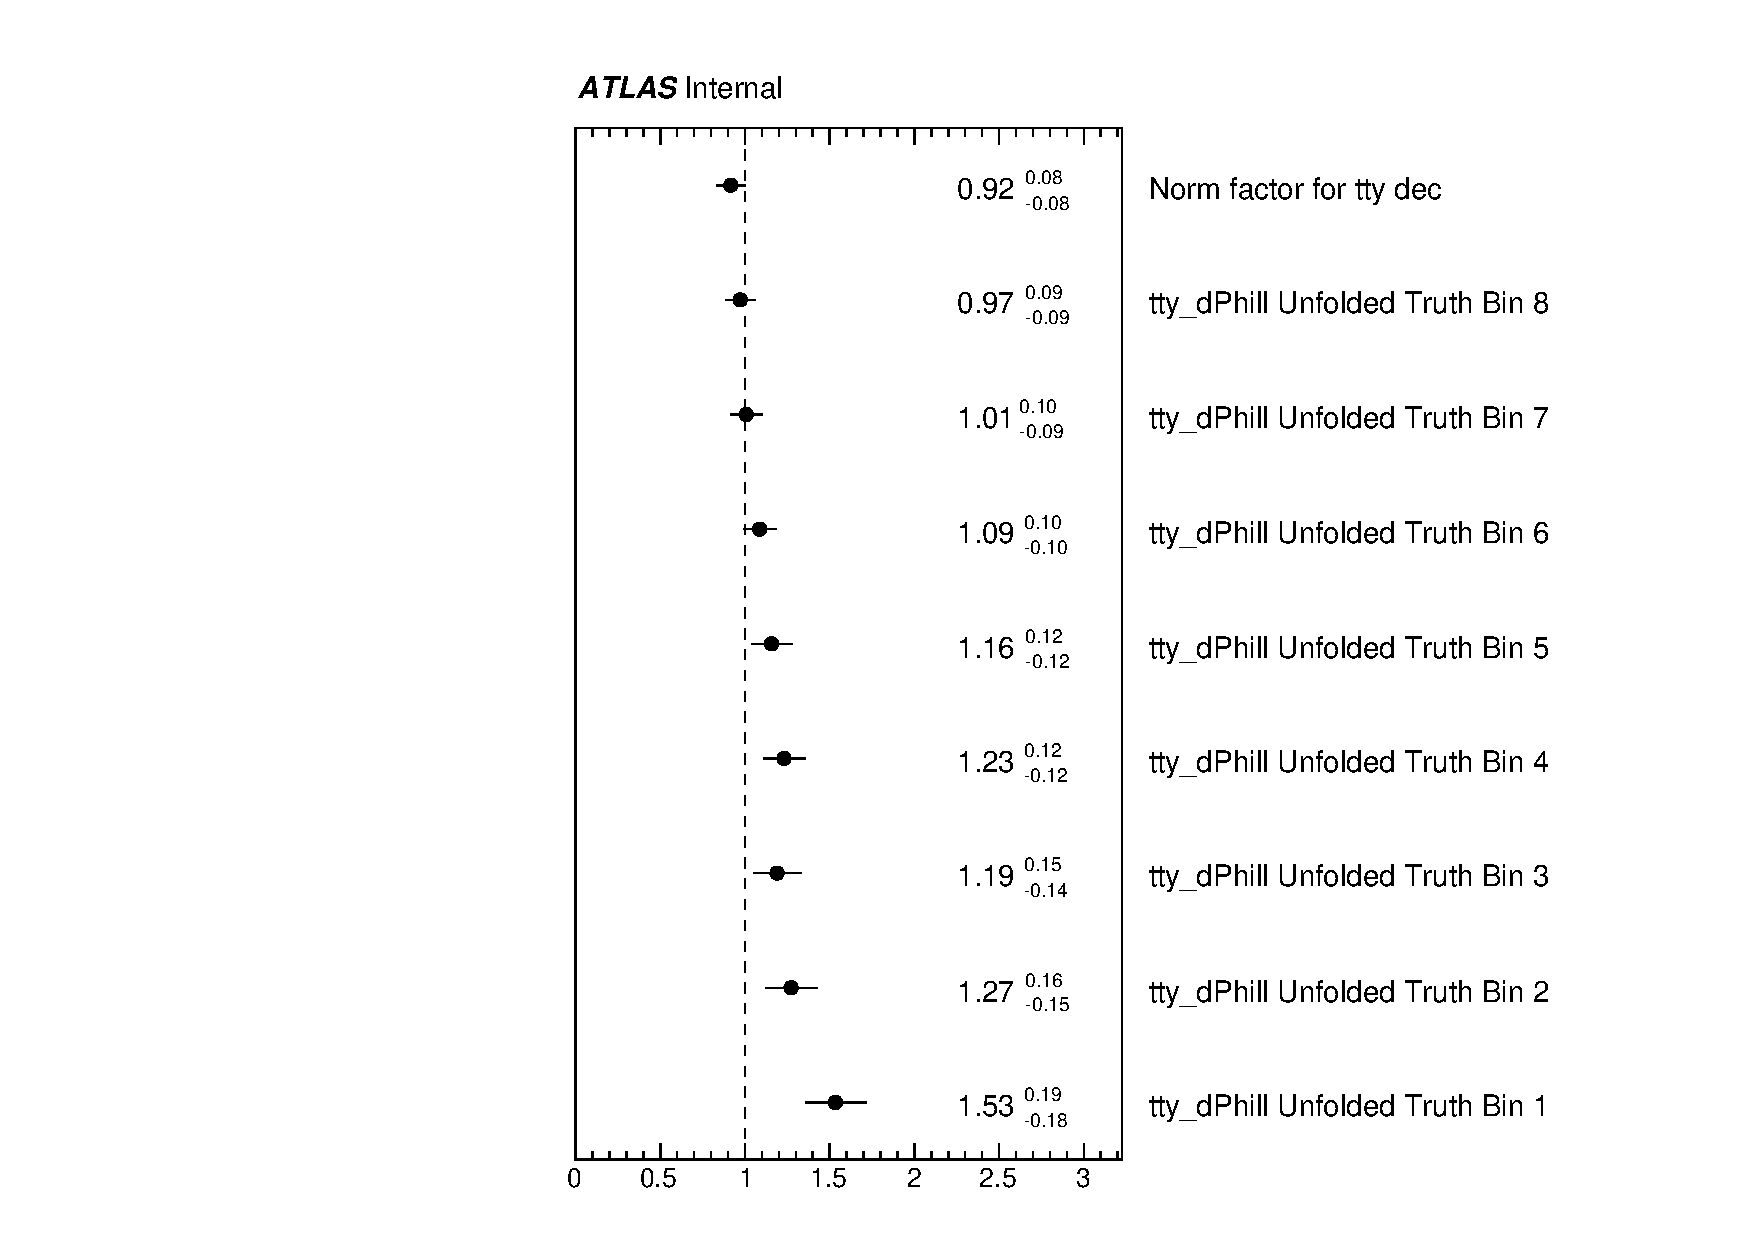
\includegraphics[width=0.3\textwidth]{figures/diff_xsec/dilep_tty_prod_mu_blinded/Unfolded_data/tty2l_dPhill_all_syst/NormFactors.pdf}}
  \quad
  \subfloat[]{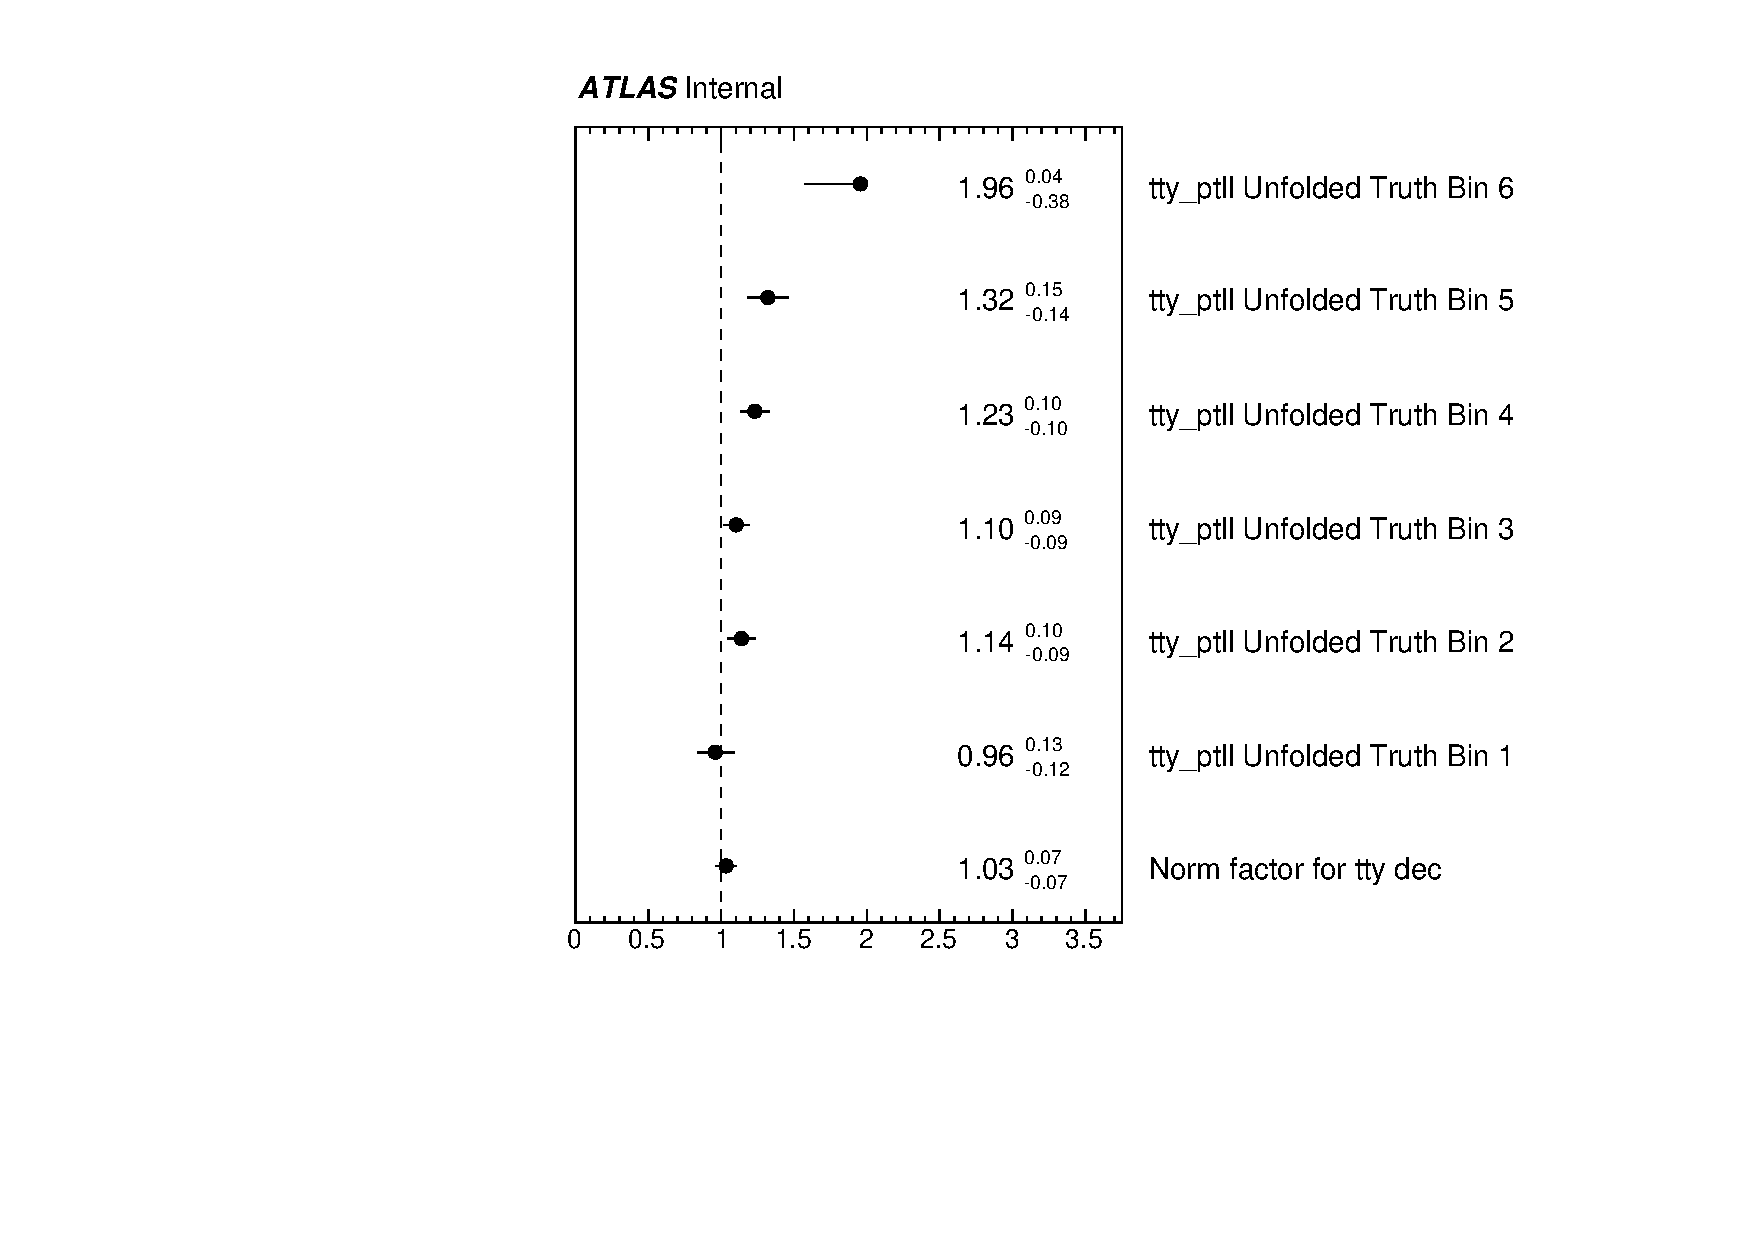
\includegraphics[width=0.3\textwidth]{figures/diff_xsec/dilep_tty_prod_mu_blinded/Unfolded_data/tty2l_ptll_all_syst/NormFactors.pdf}}
  \quad
  \subfloat[]{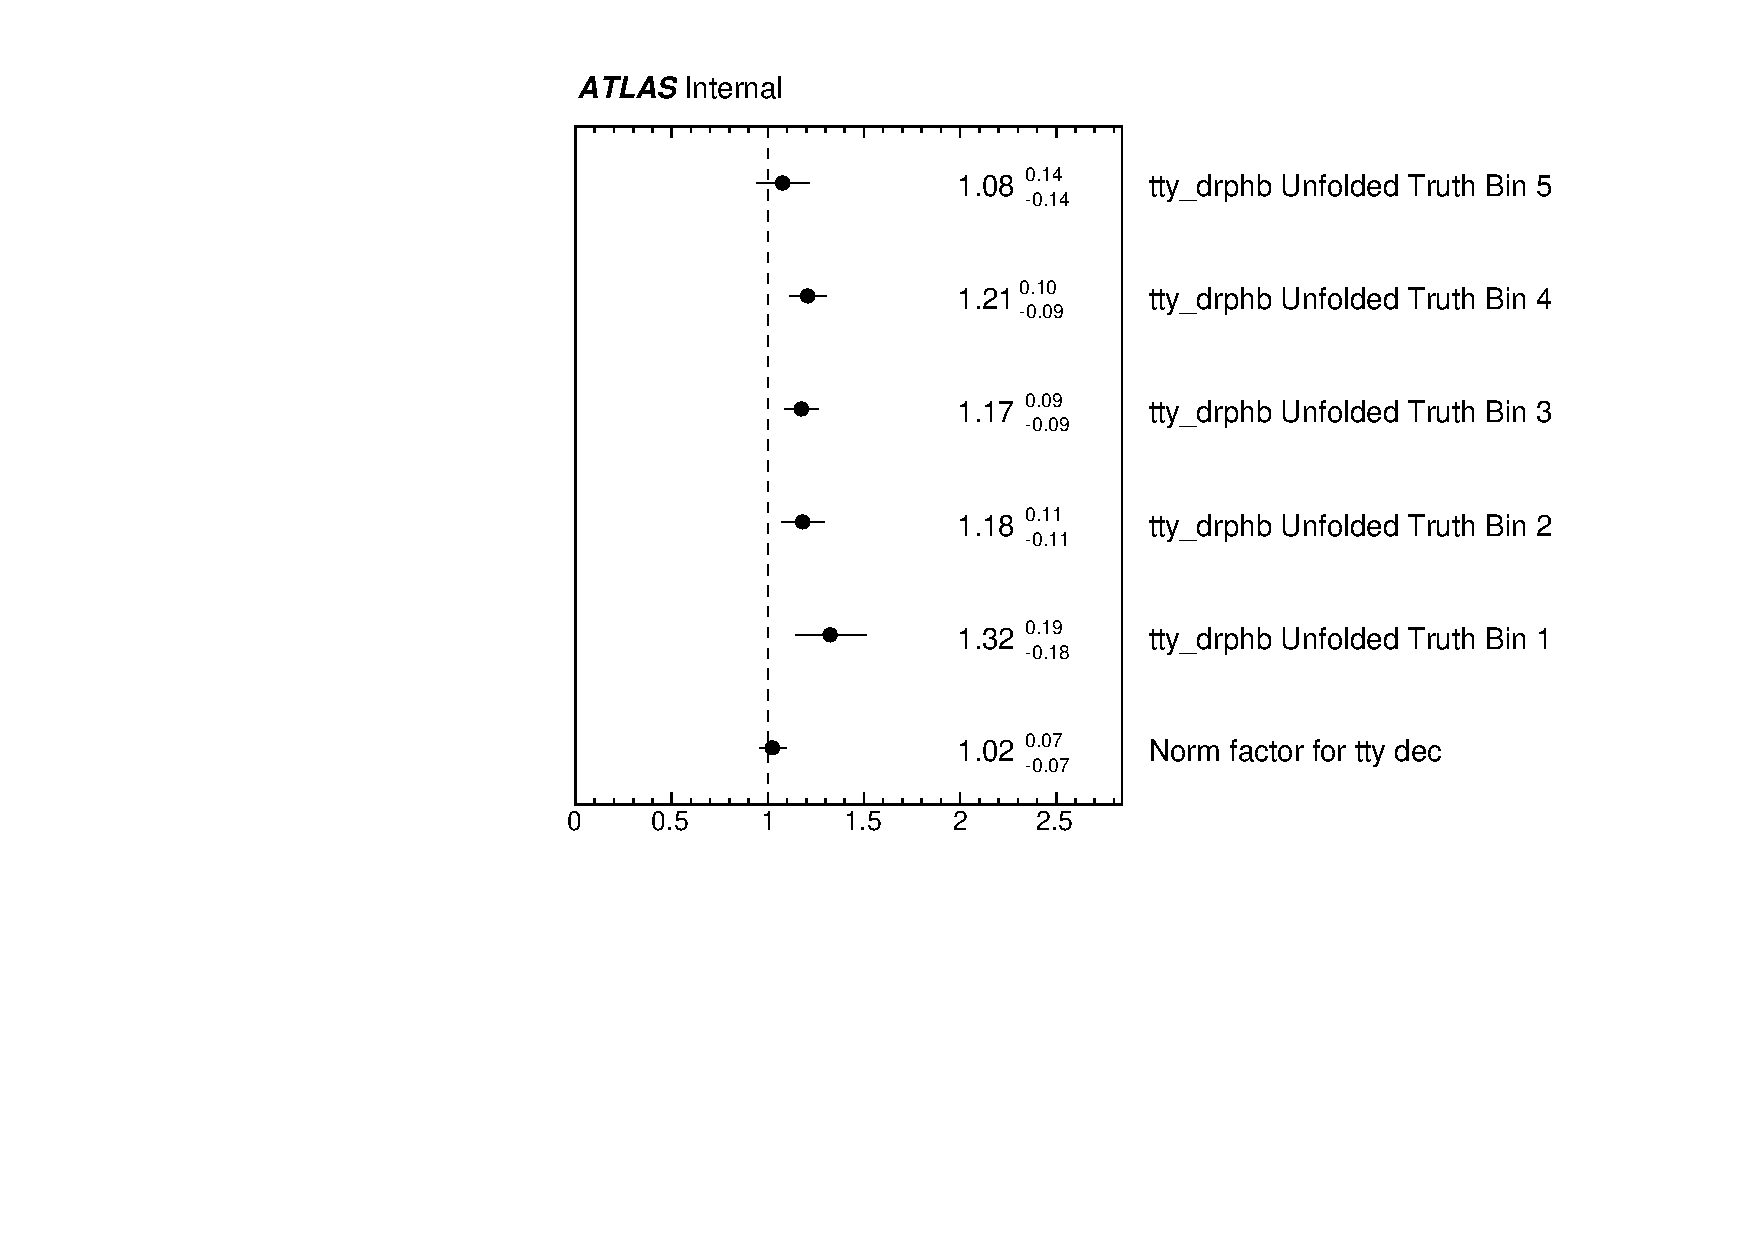
\includegraphics[width=0.3\textwidth]{figures/diff_xsec/dilep_tty_prod_mu_blinded/Unfolded_data/tty2l_drphb_all_syst/NormFactors.pdf}}
  \quad
  \subfloat[]{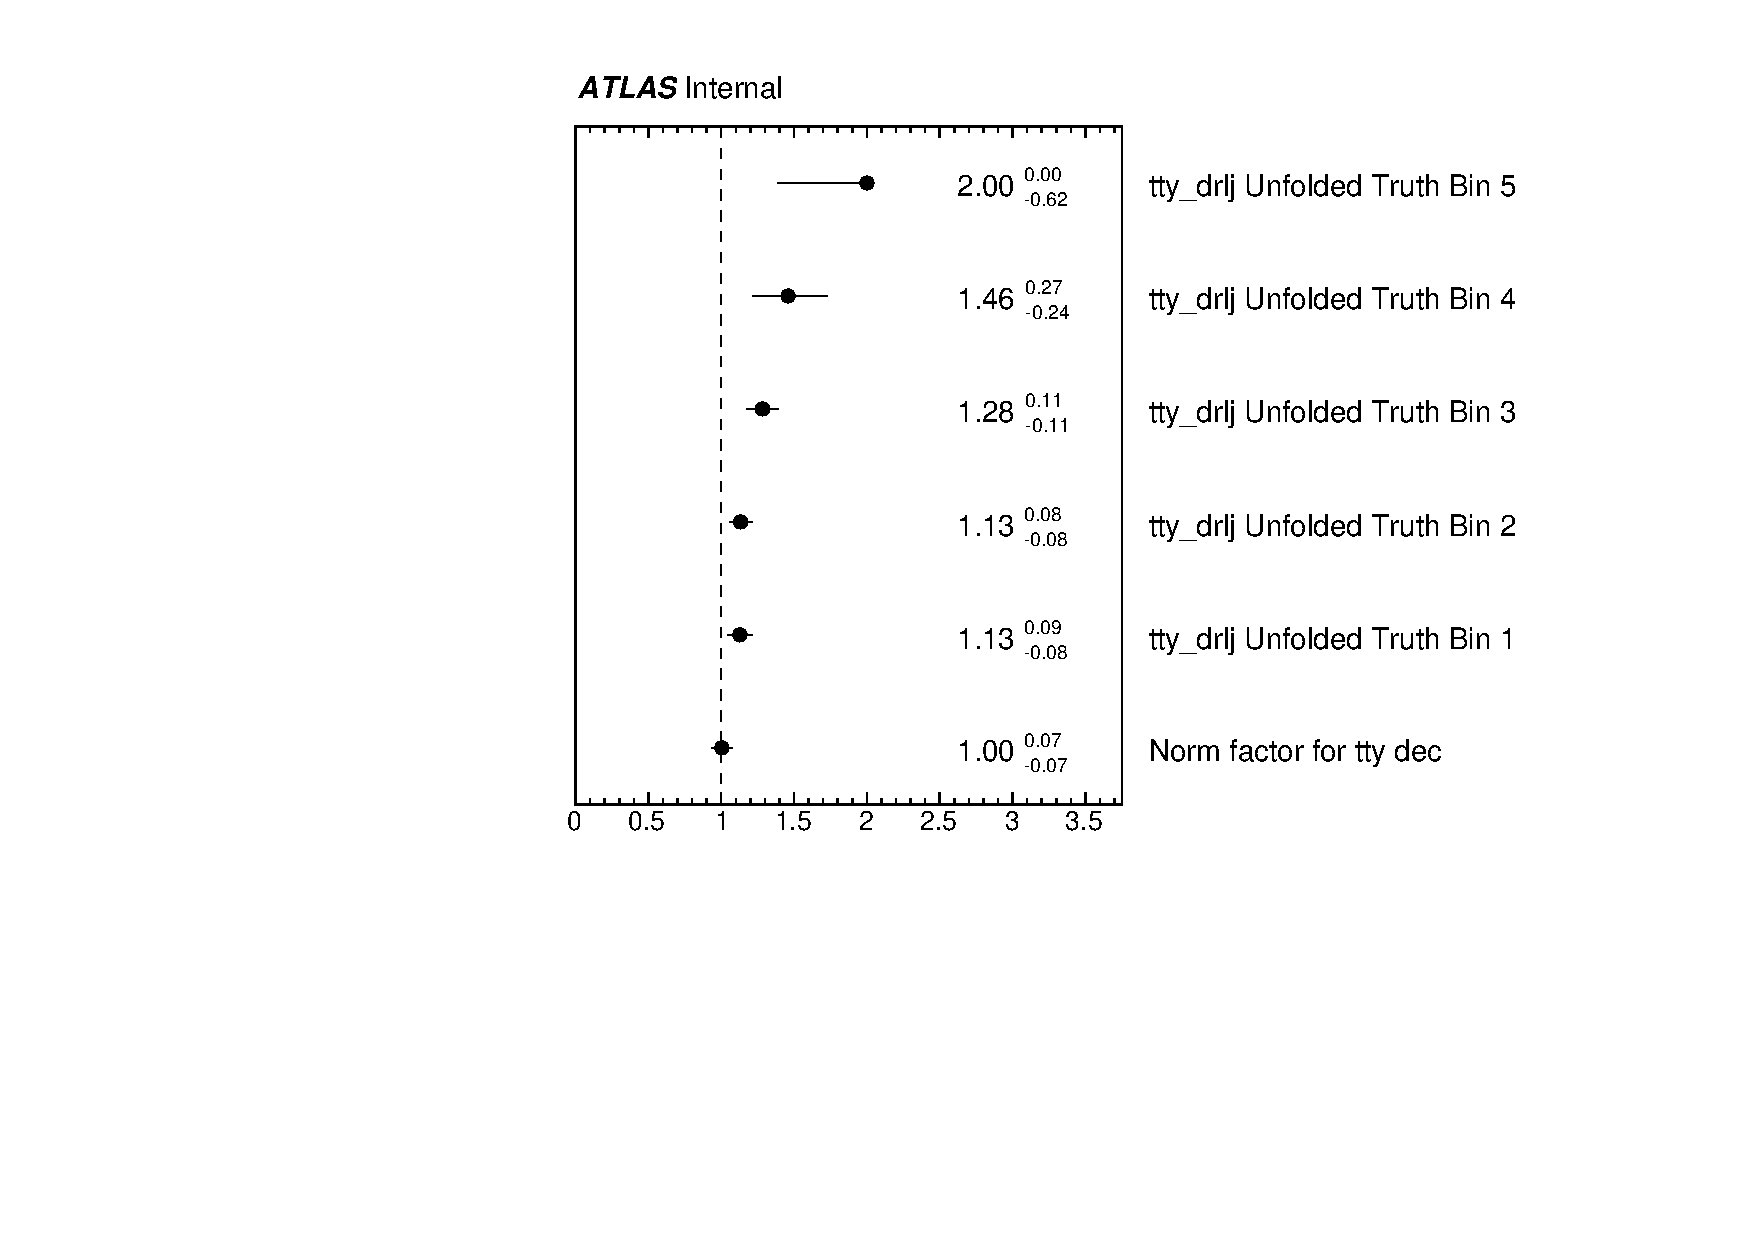
\includegraphics[width=0.3\textwidth]{figures/diff_xsec/dilep_tty_prod_mu_blinded/Unfolded_data/tty2l_drlj_all_syst/NormFactors.pdf}}
  \quad
  \subfloat[]{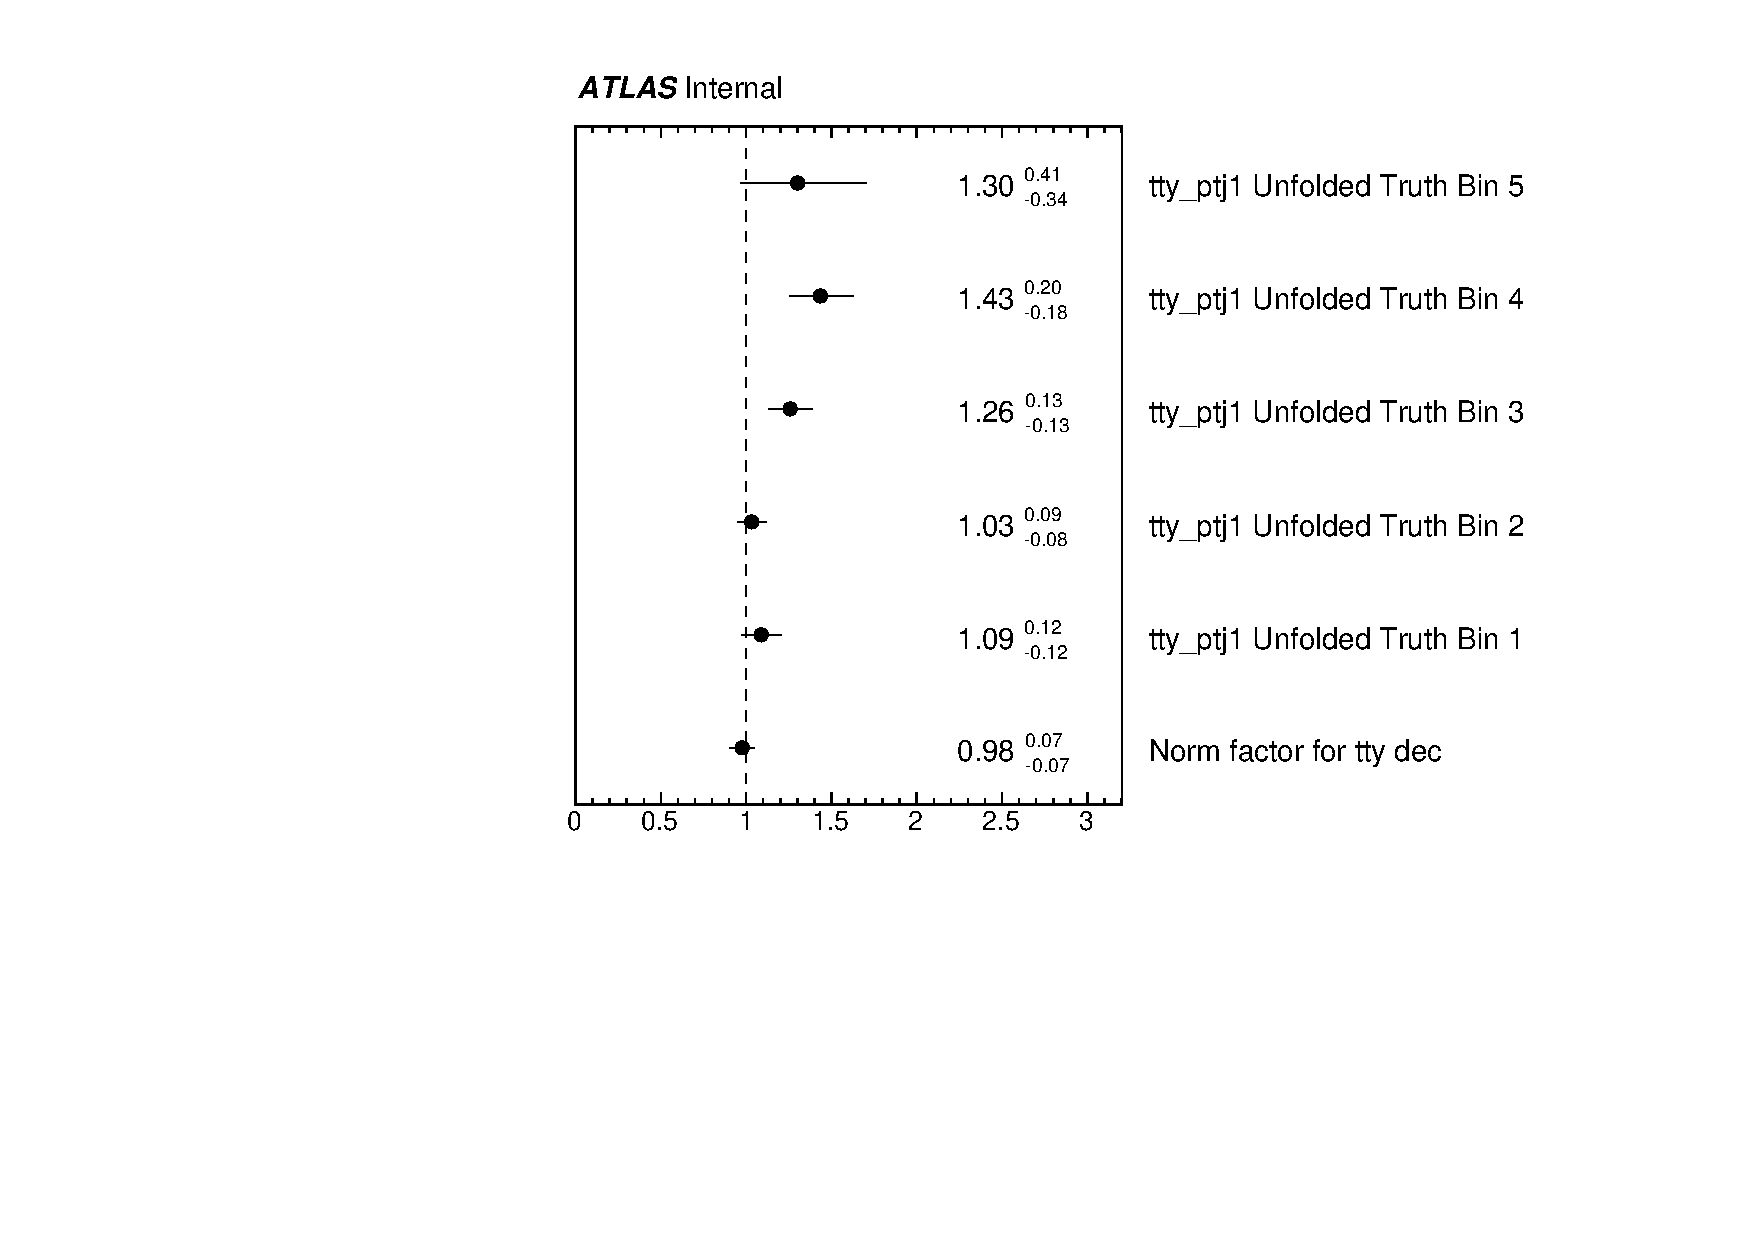
\includegraphics[width=0.3\textwidth]{figures/diff_xsec/dilep_tty_prod_mu_blinded/Unfolded_data/tty2l_ptj1_all_syst/NormFactors.pdf}}
  \caption{ The figure displays the normalisation factors obtained from the fit for \tty production measurement in dilepton channel for the following observables: (a) $p_T(\gamma)$, (b) $|\eta(\gamma|)$, (c) $\Delta R_{min}(\gamma, l)$, (d) $\Delta R(\gamma, l1)$, (e) $\Delta R(\gamma, l2)$, (f) $|\Delta \eta(l, l)|$, (g) $|\Delta \phi(l, l)|$, (h) $p_T(ll)$, (i) $\Delta R(\gamma, b)$, (j) $\Delta R_{min}(l, j)$, (k) $p_T(j1)$.}
  \label{fig:pt_unfolded_dilep_table_realdata}
\end{figure}
\FloatBarrier


\begin{figure}[ht]
  \centering
  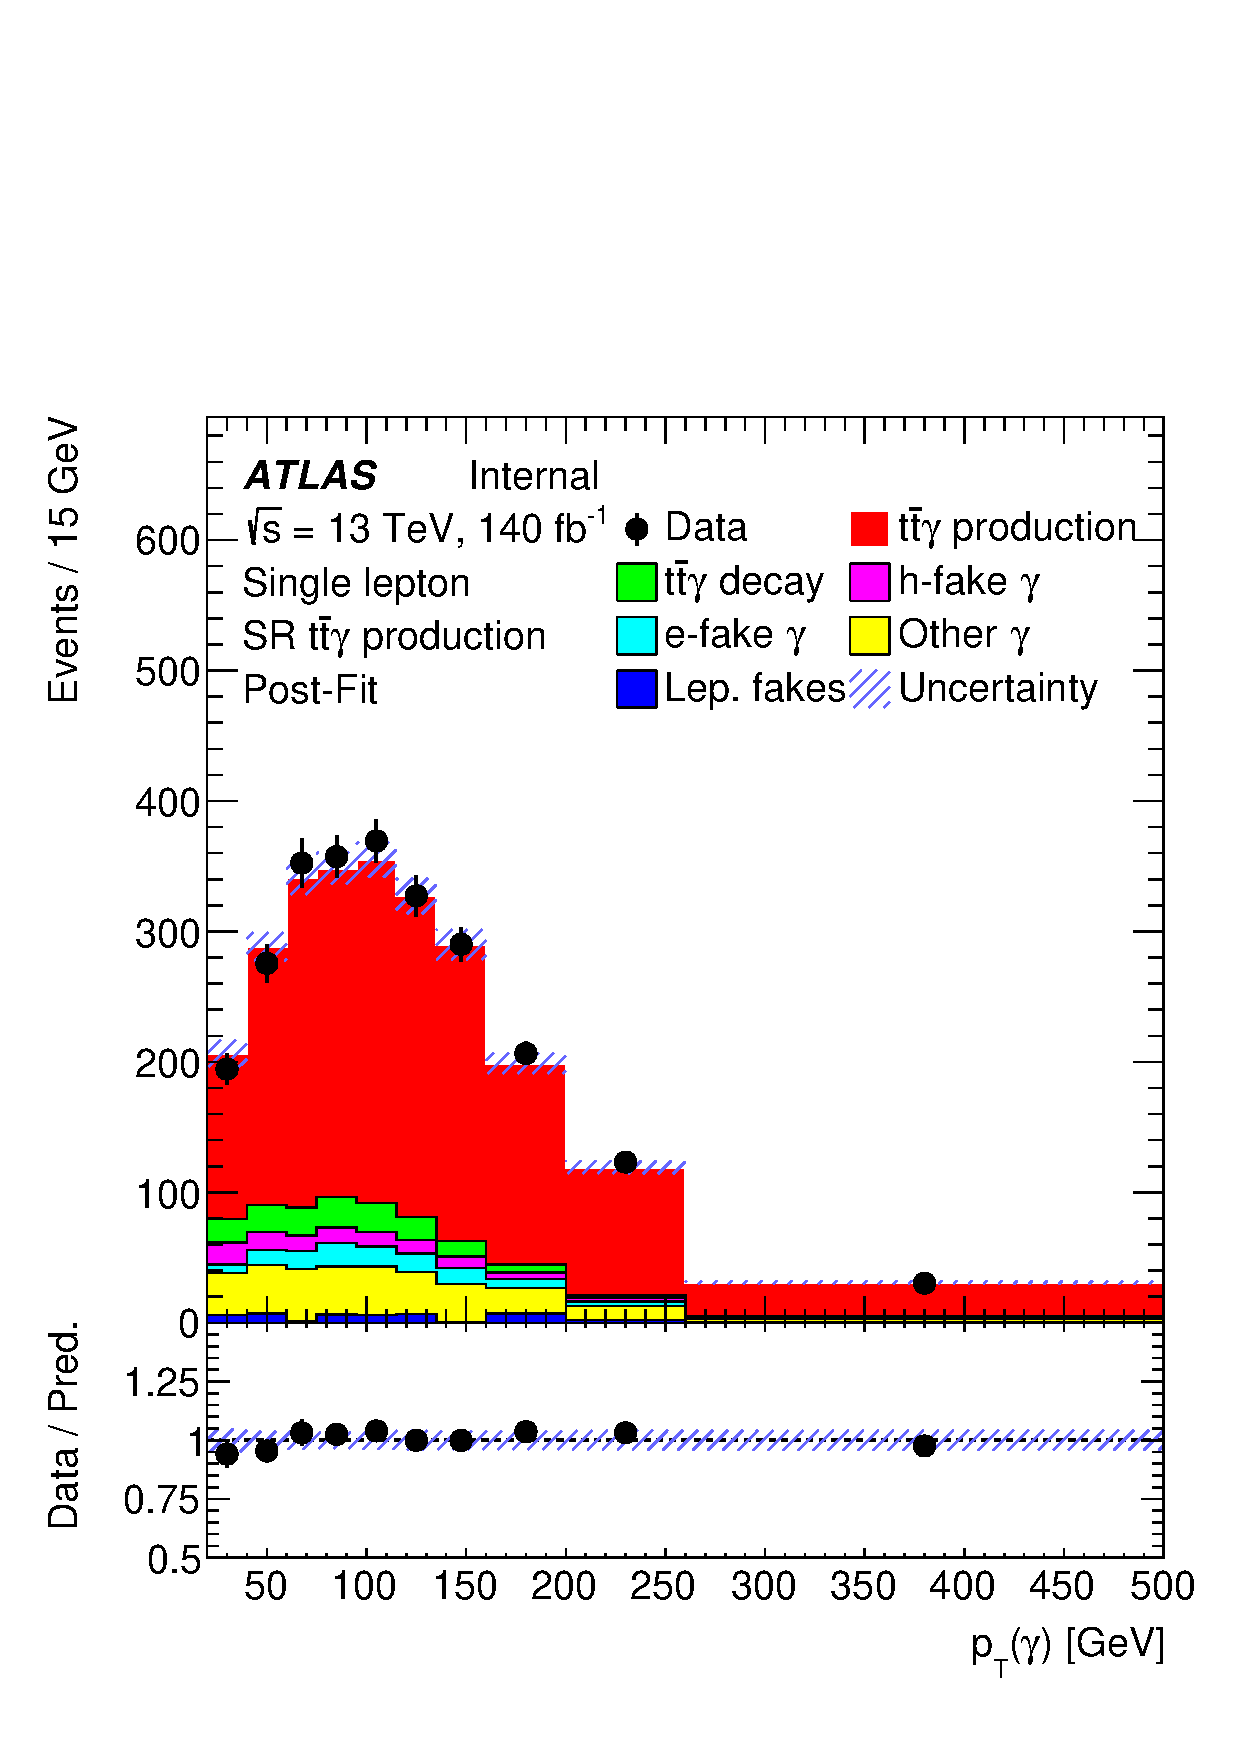
\includegraphics[width=0.25\textwidth]{figures/diff_xsec/ljet/post_fit/tty1l_pt_all_syst/Plots/SR1_postFit.pdf}%
  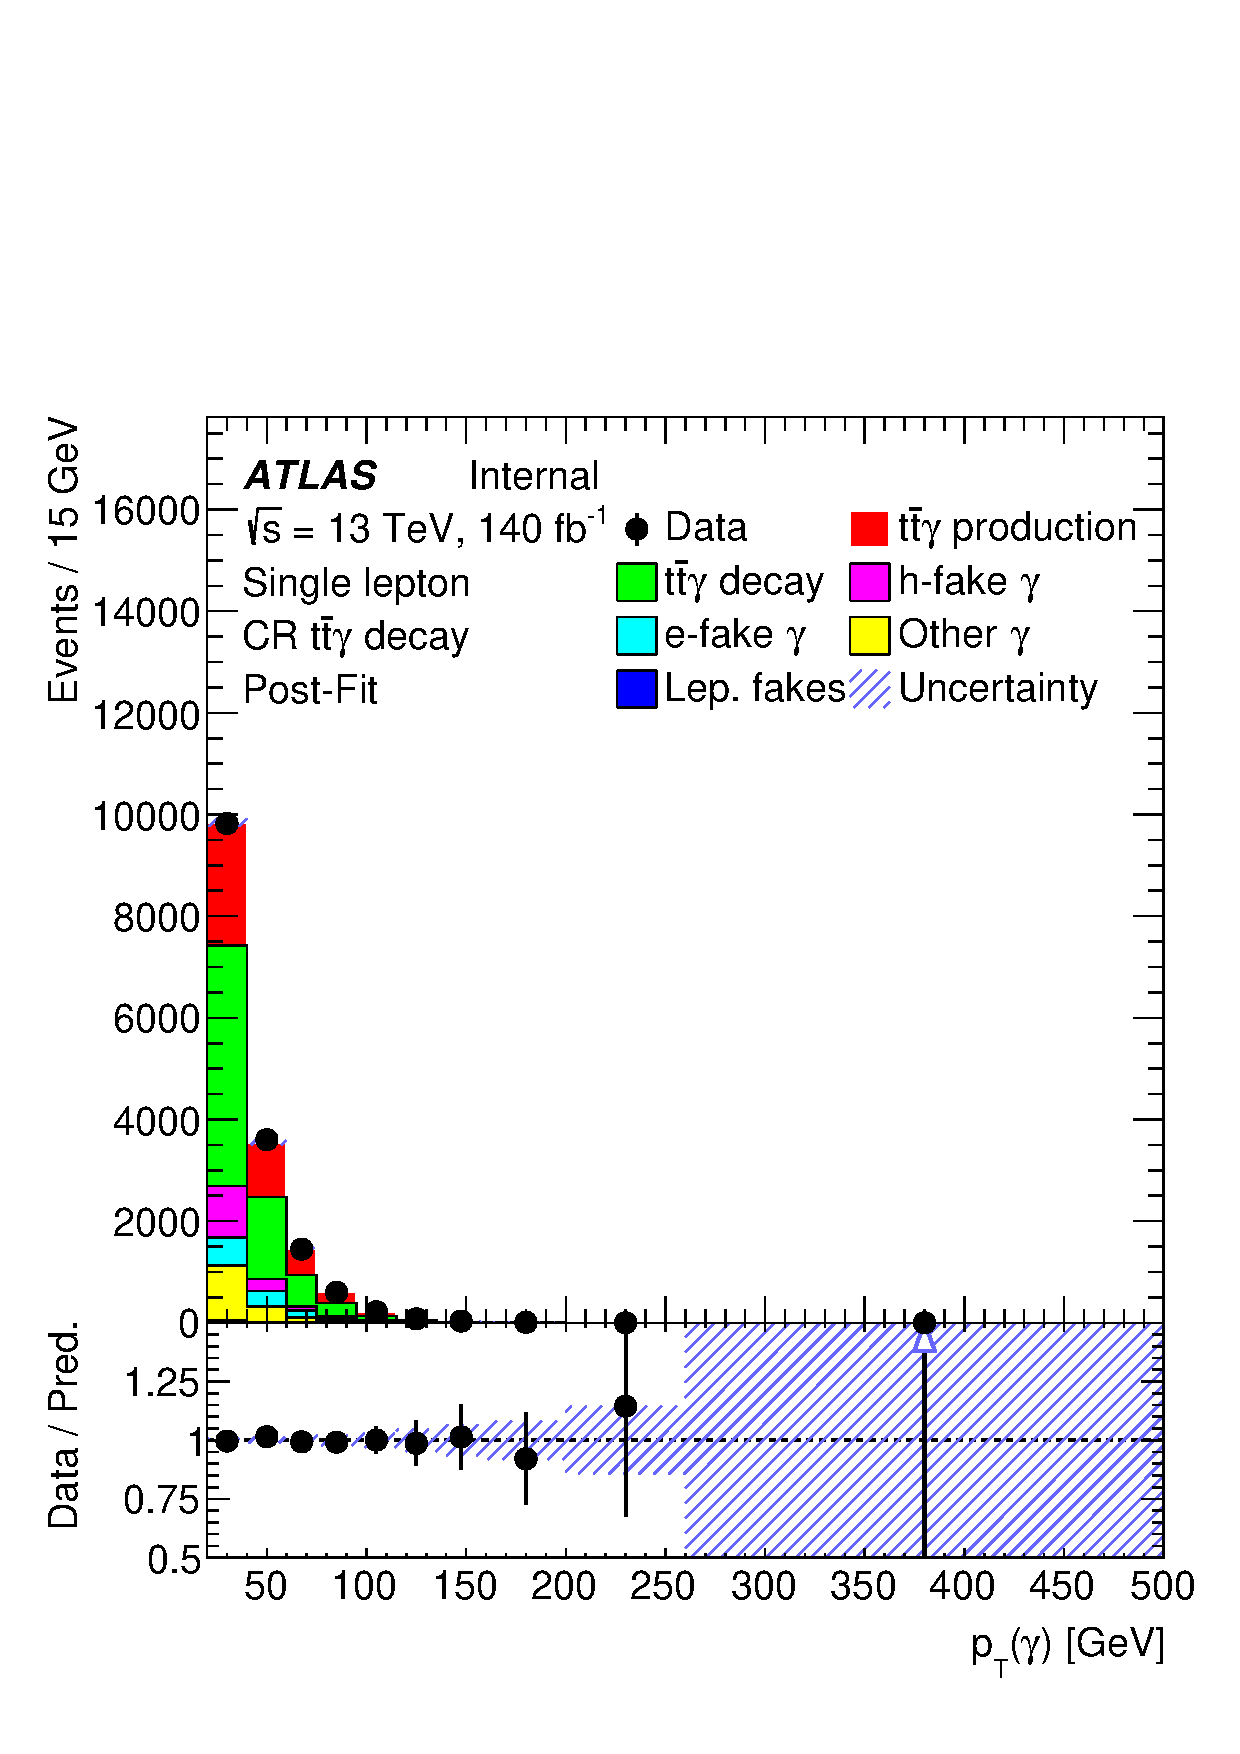
\includegraphics[width=0.25\textwidth]{figures/diff_xsec/ljet/post_fit/tty1l_pt_all_syst/Plots/SR2_postFit.pdf}%
  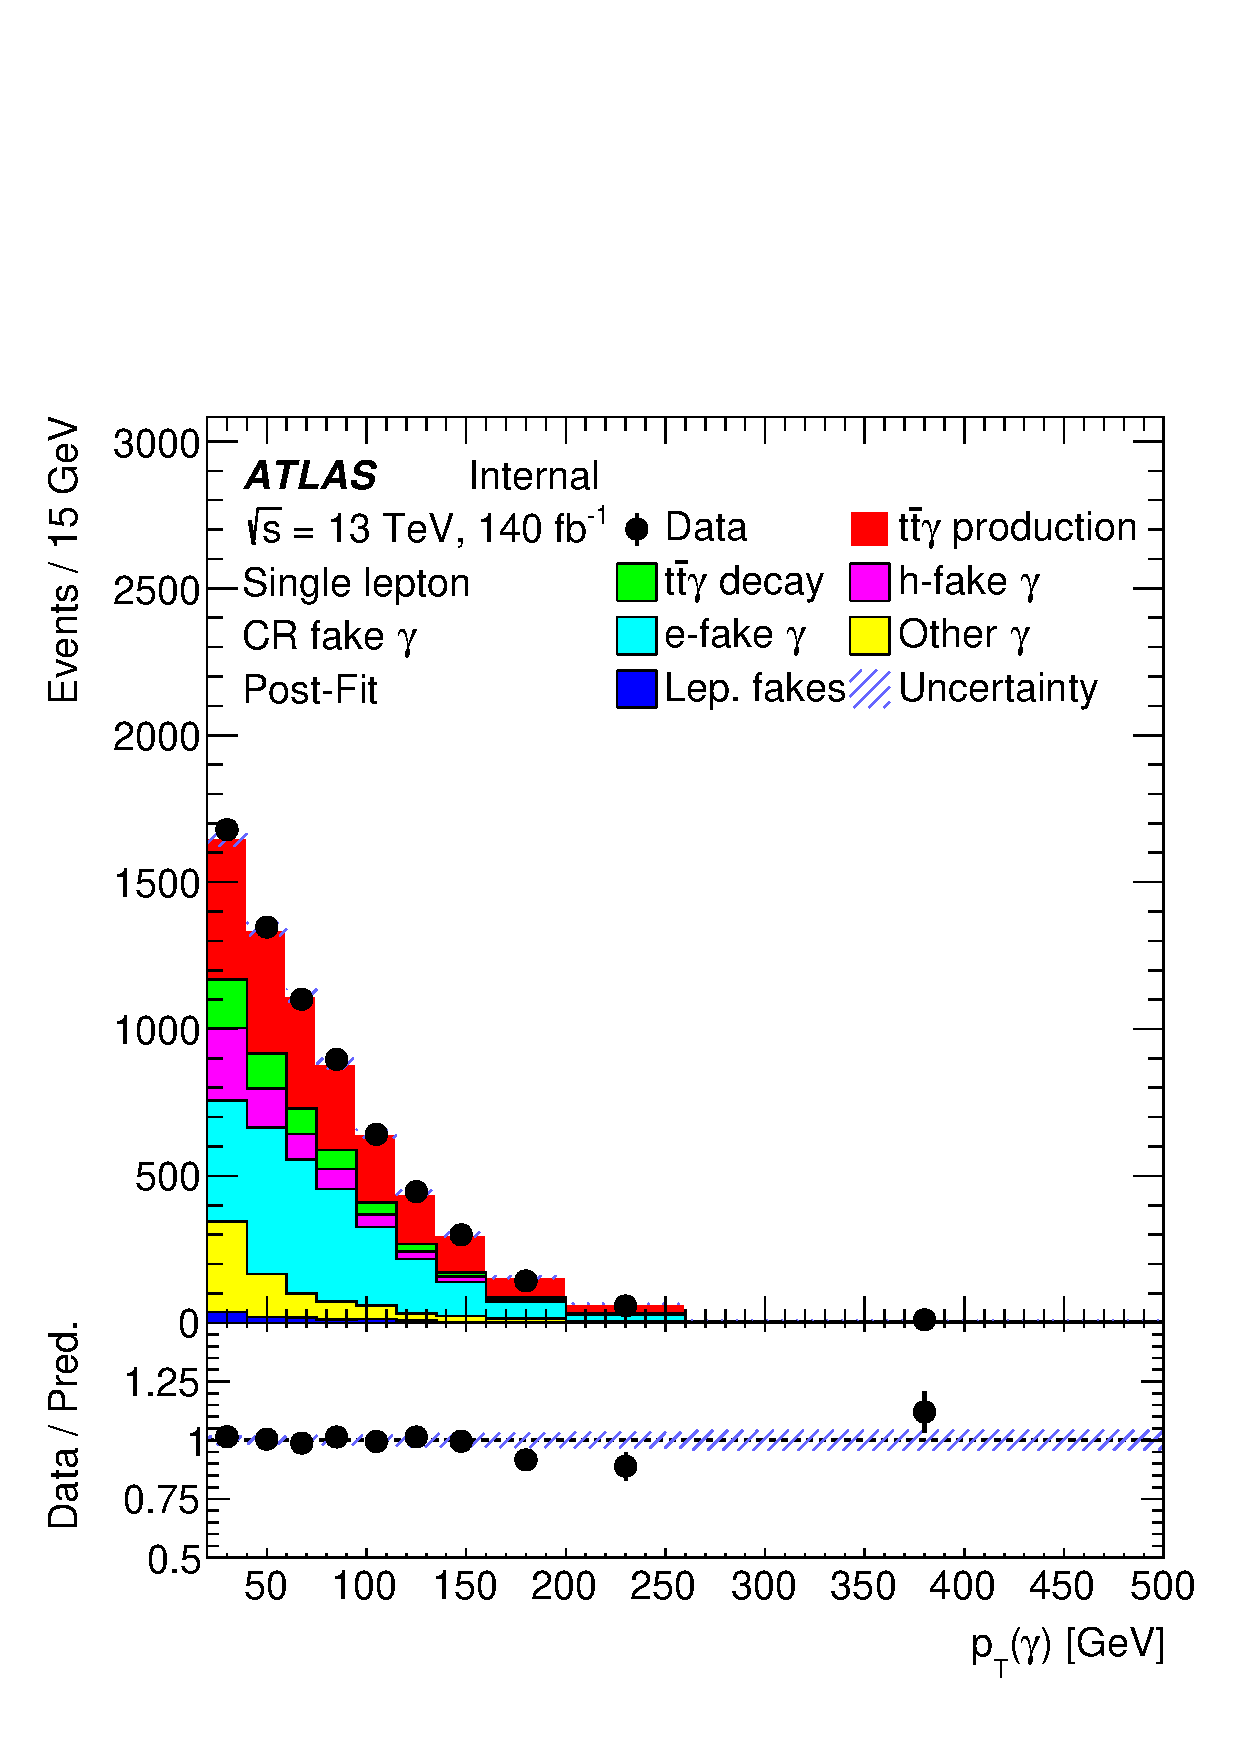
\includegraphics[width=0.25\textwidth]{figures/diff_xsec/ljet/post_fit/tty1l_pt_all_syst/Plots/SR3_postFit.pdf}%
  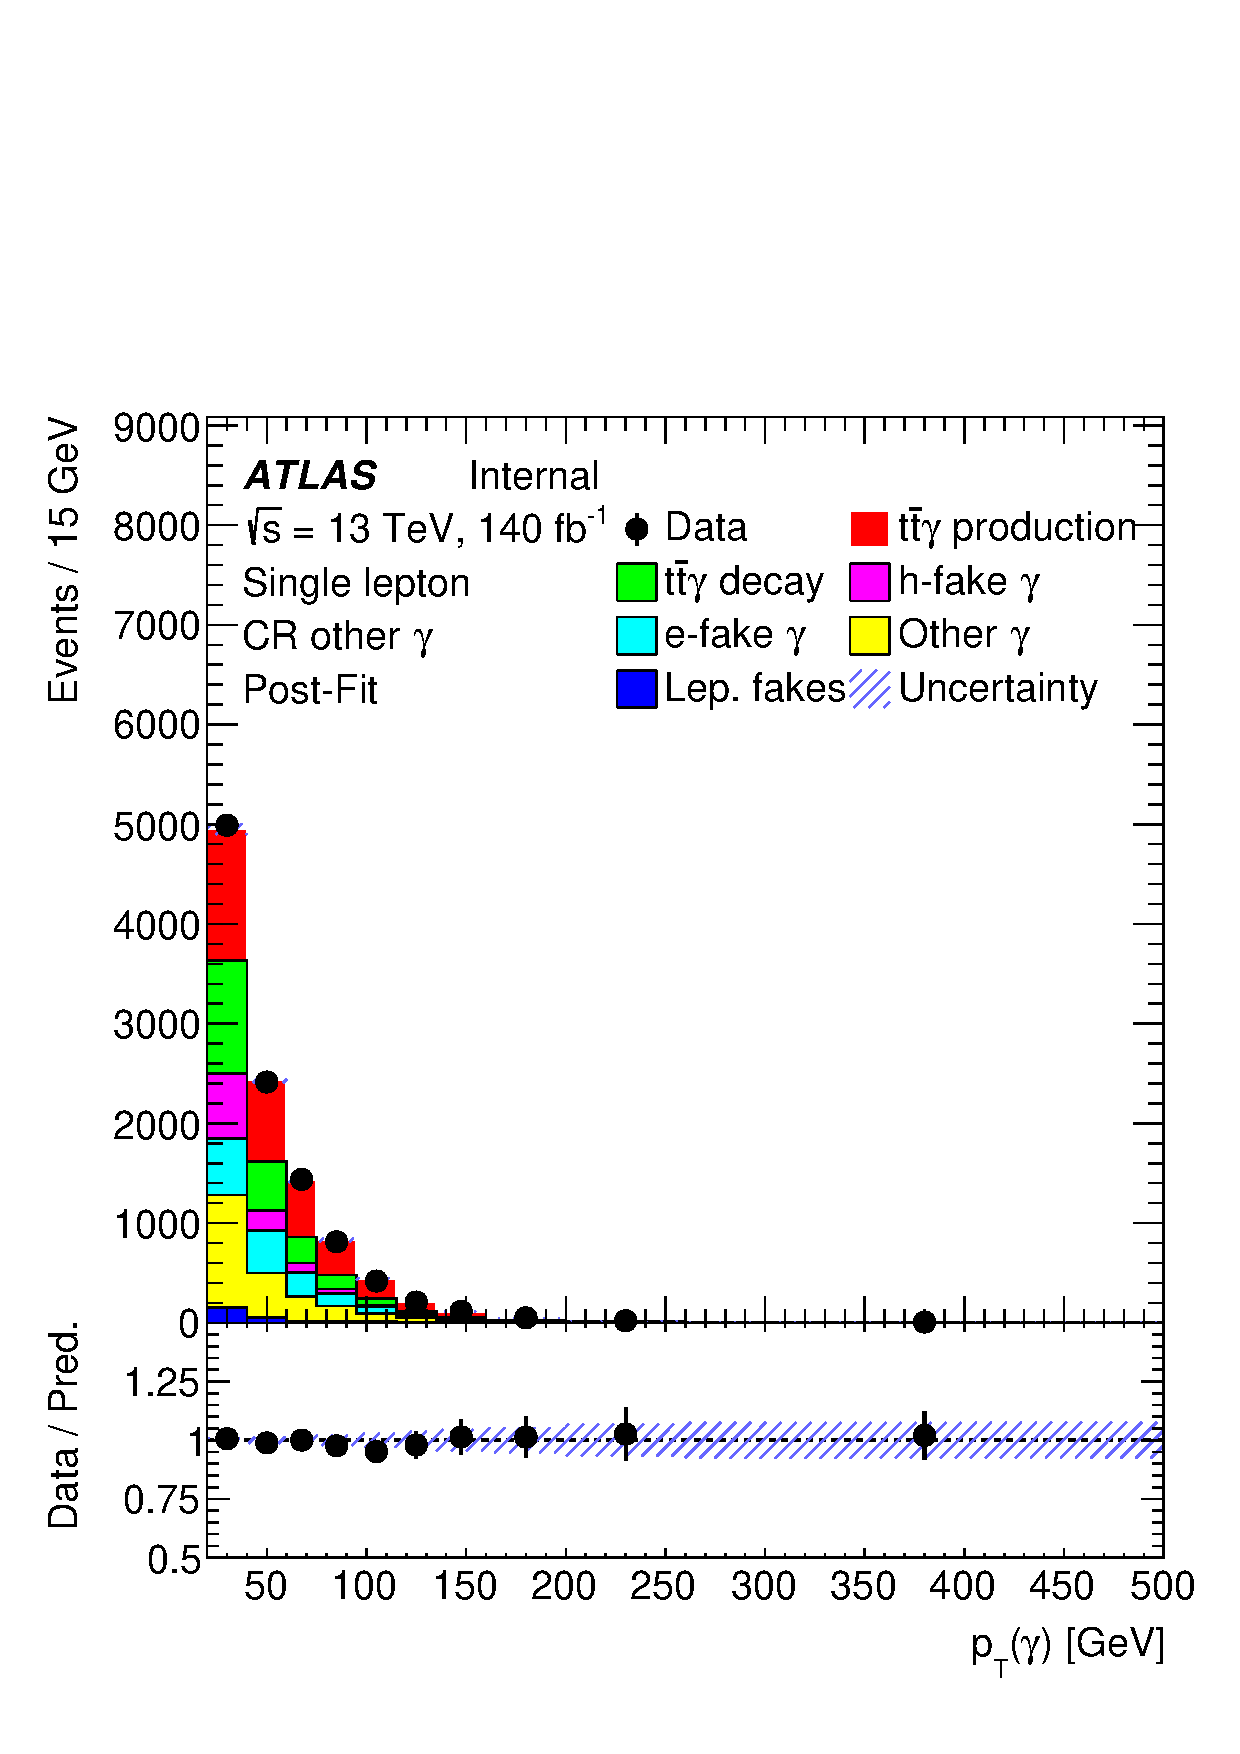
\includegraphics[width=0.25\textwidth]{figures/diff_xsec/ljet/post_fit/tty1l_pt_all_syst/Plots/SR4_postFit.pdf}%
  \caption{The post-fit distributions of \ptgamma in 4 regions, \tty production enriched region, \tty decay enriched region, fakes enriched region, prompt photon enriched region (from left to right) in single lepton channel. }
  \label{fig:pt_postfit_ljet_realdata}
\end{figure}
\FloatBarrier


\begin{figure}[ht]
  \centering
  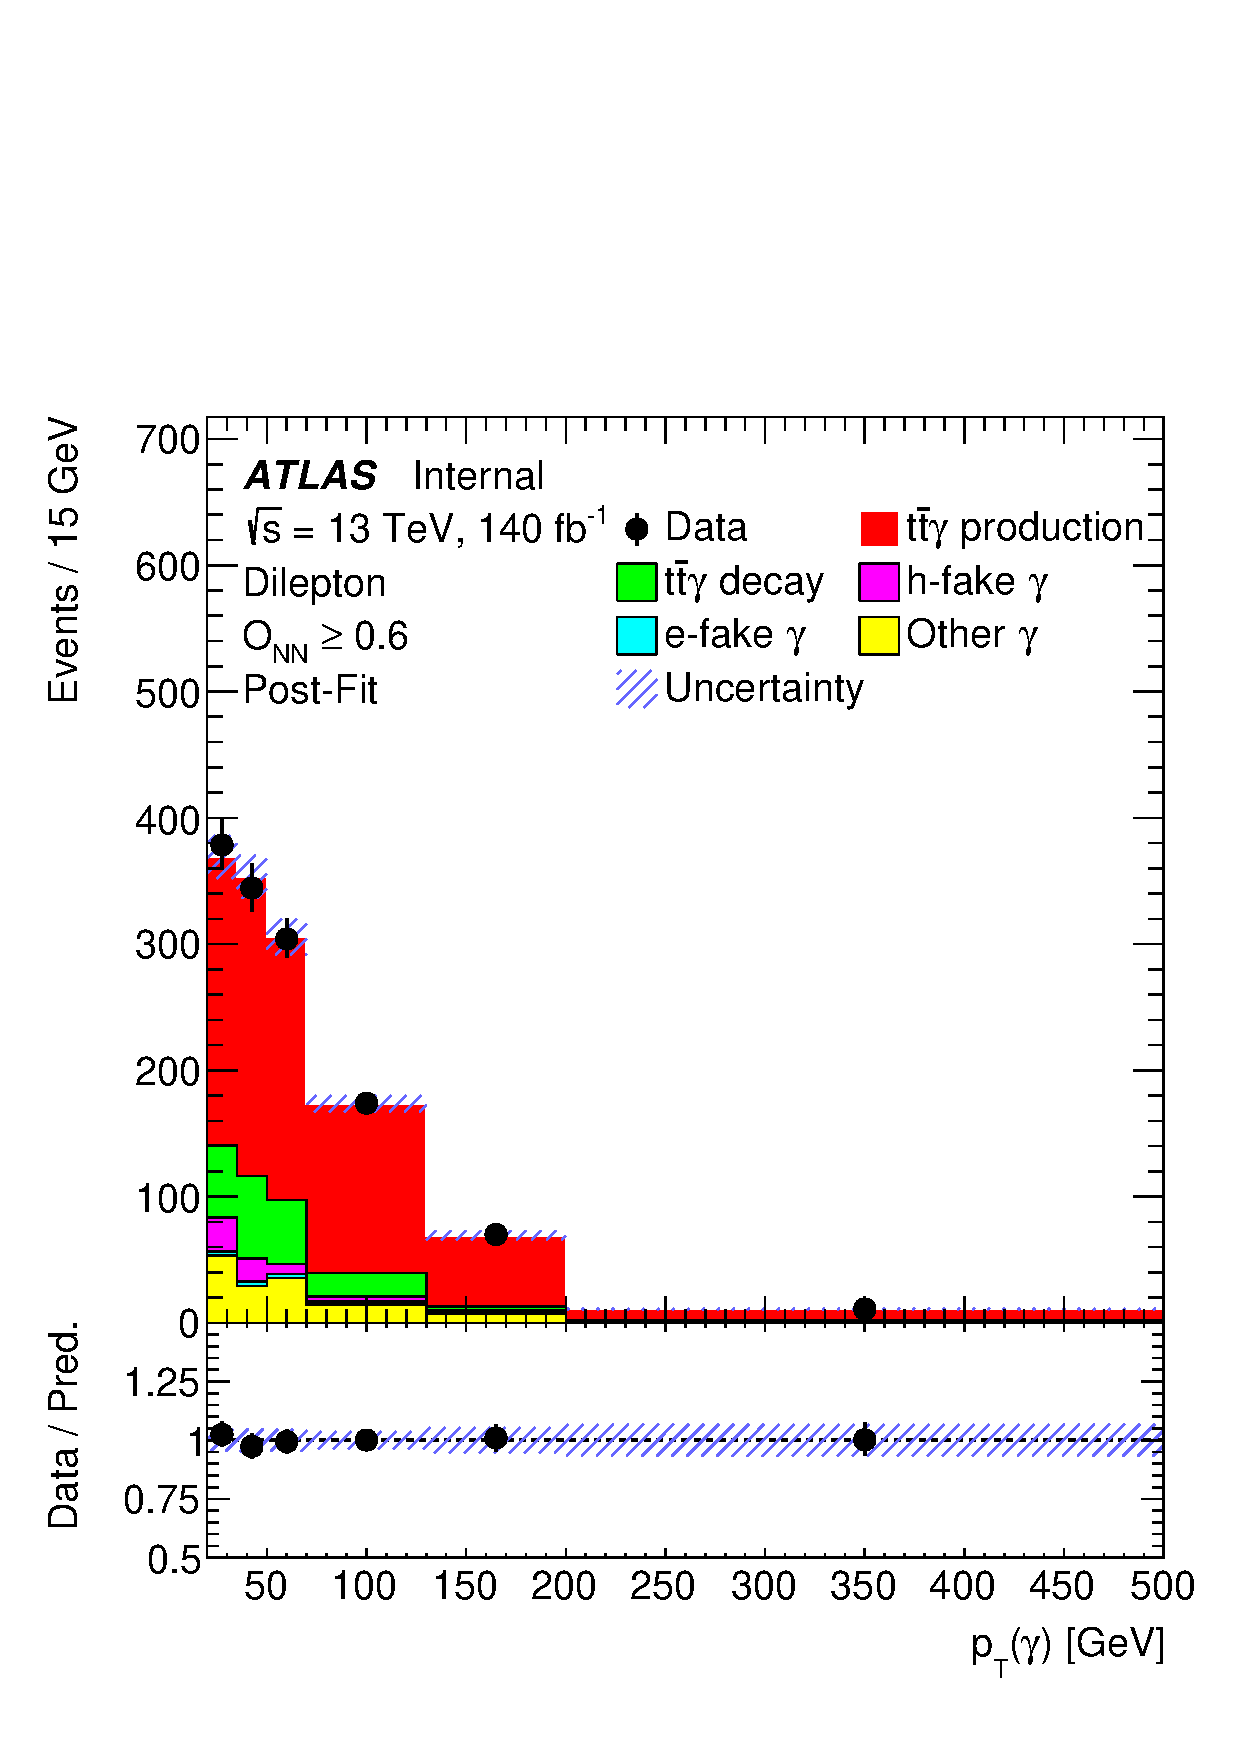
\includegraphics[width=0.25\textwidth]{figures/diff_xsec/dilep/post_fit/tty2l_pt_all_syst/Plots/SR1_postFit.pdf}%
  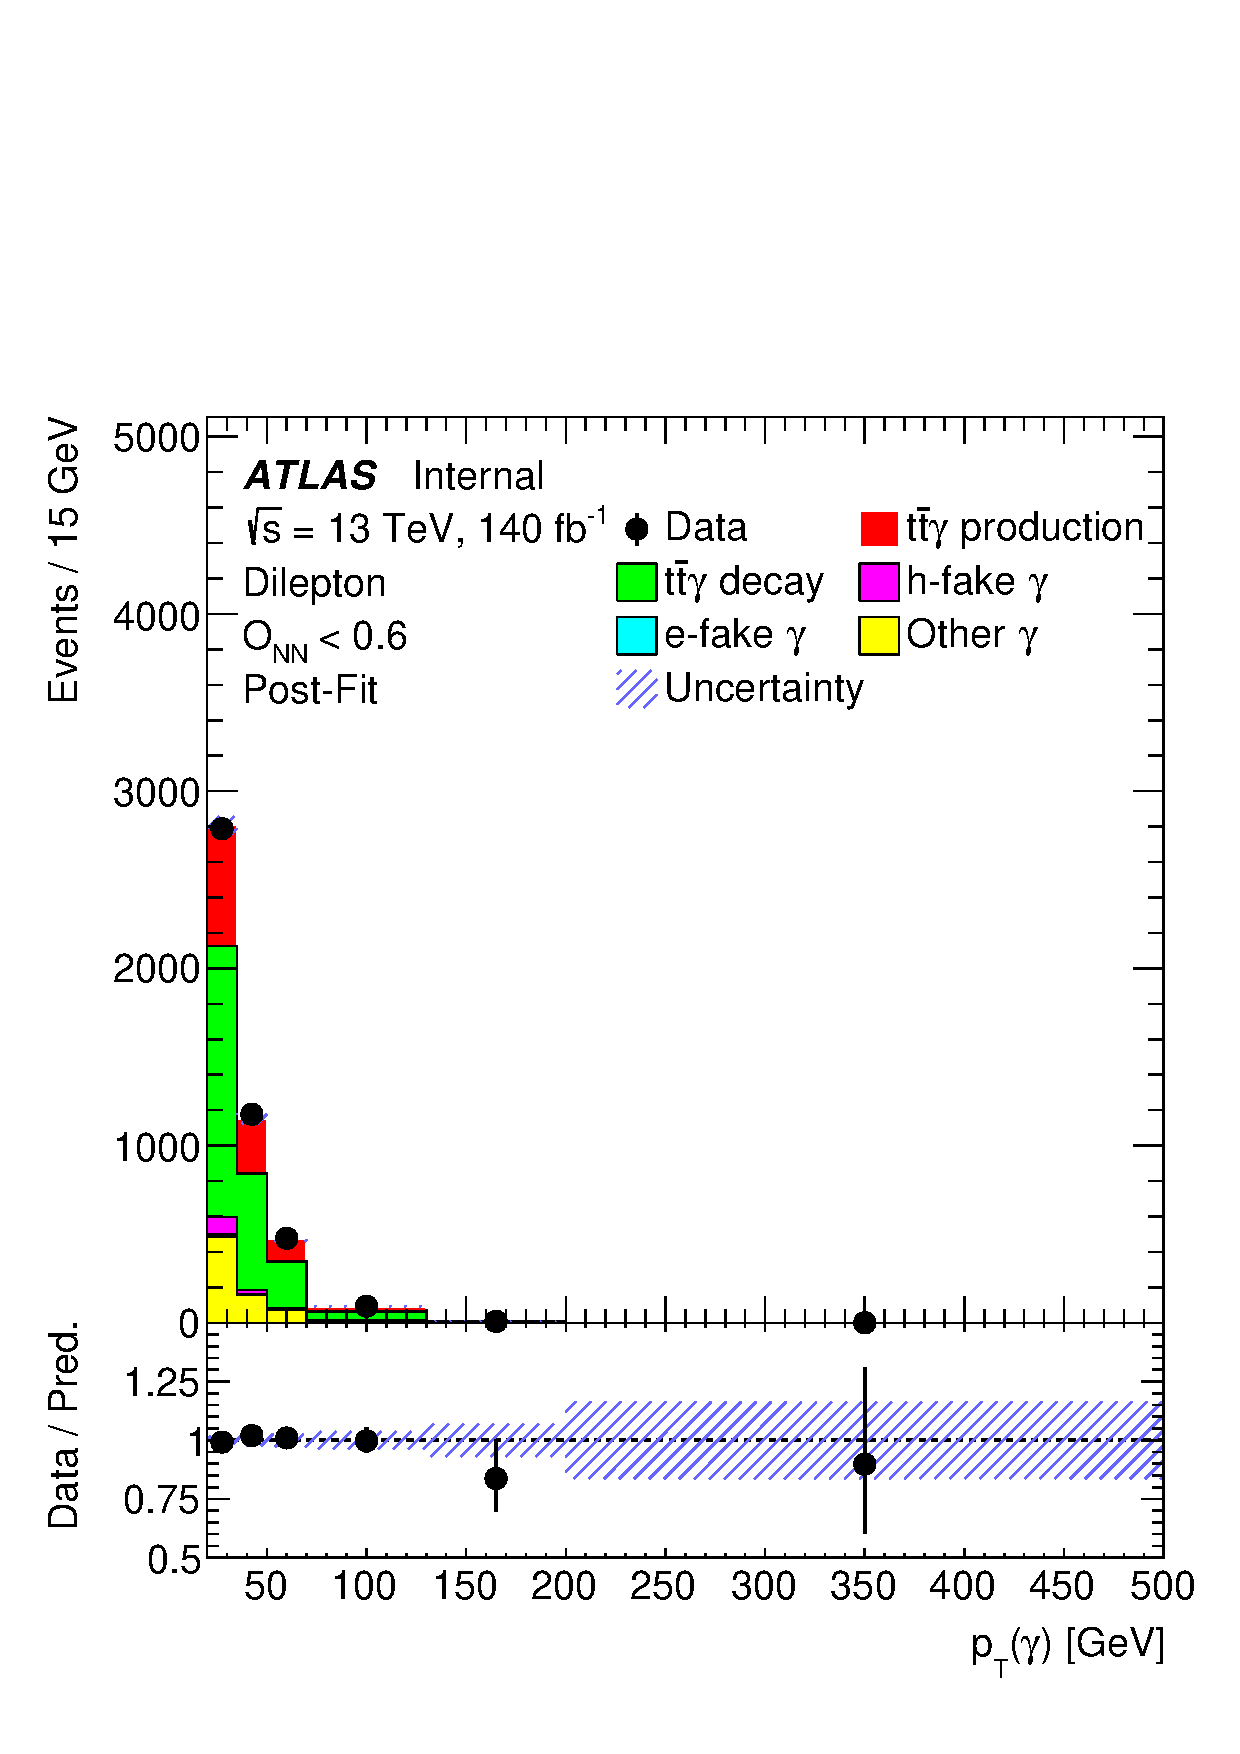
\includegraphics[width=0.25\textwidth]{figures/diff_xsec/dilep/post_fit/tty2l_pt_all_syst/Plots/SR2_postFit.pdf}%
  \caption{The post-fit distributions of \ptgamma in two regions $O_{NN}>=0.6$, $O_{NN}<0.6$ in dilepton channel (from left to right).}
  \label{fig:pt_postfit_dilep_realdata}
\end{figure}
\FloatBarrier


\begin{figure}[ht]
  \centering
  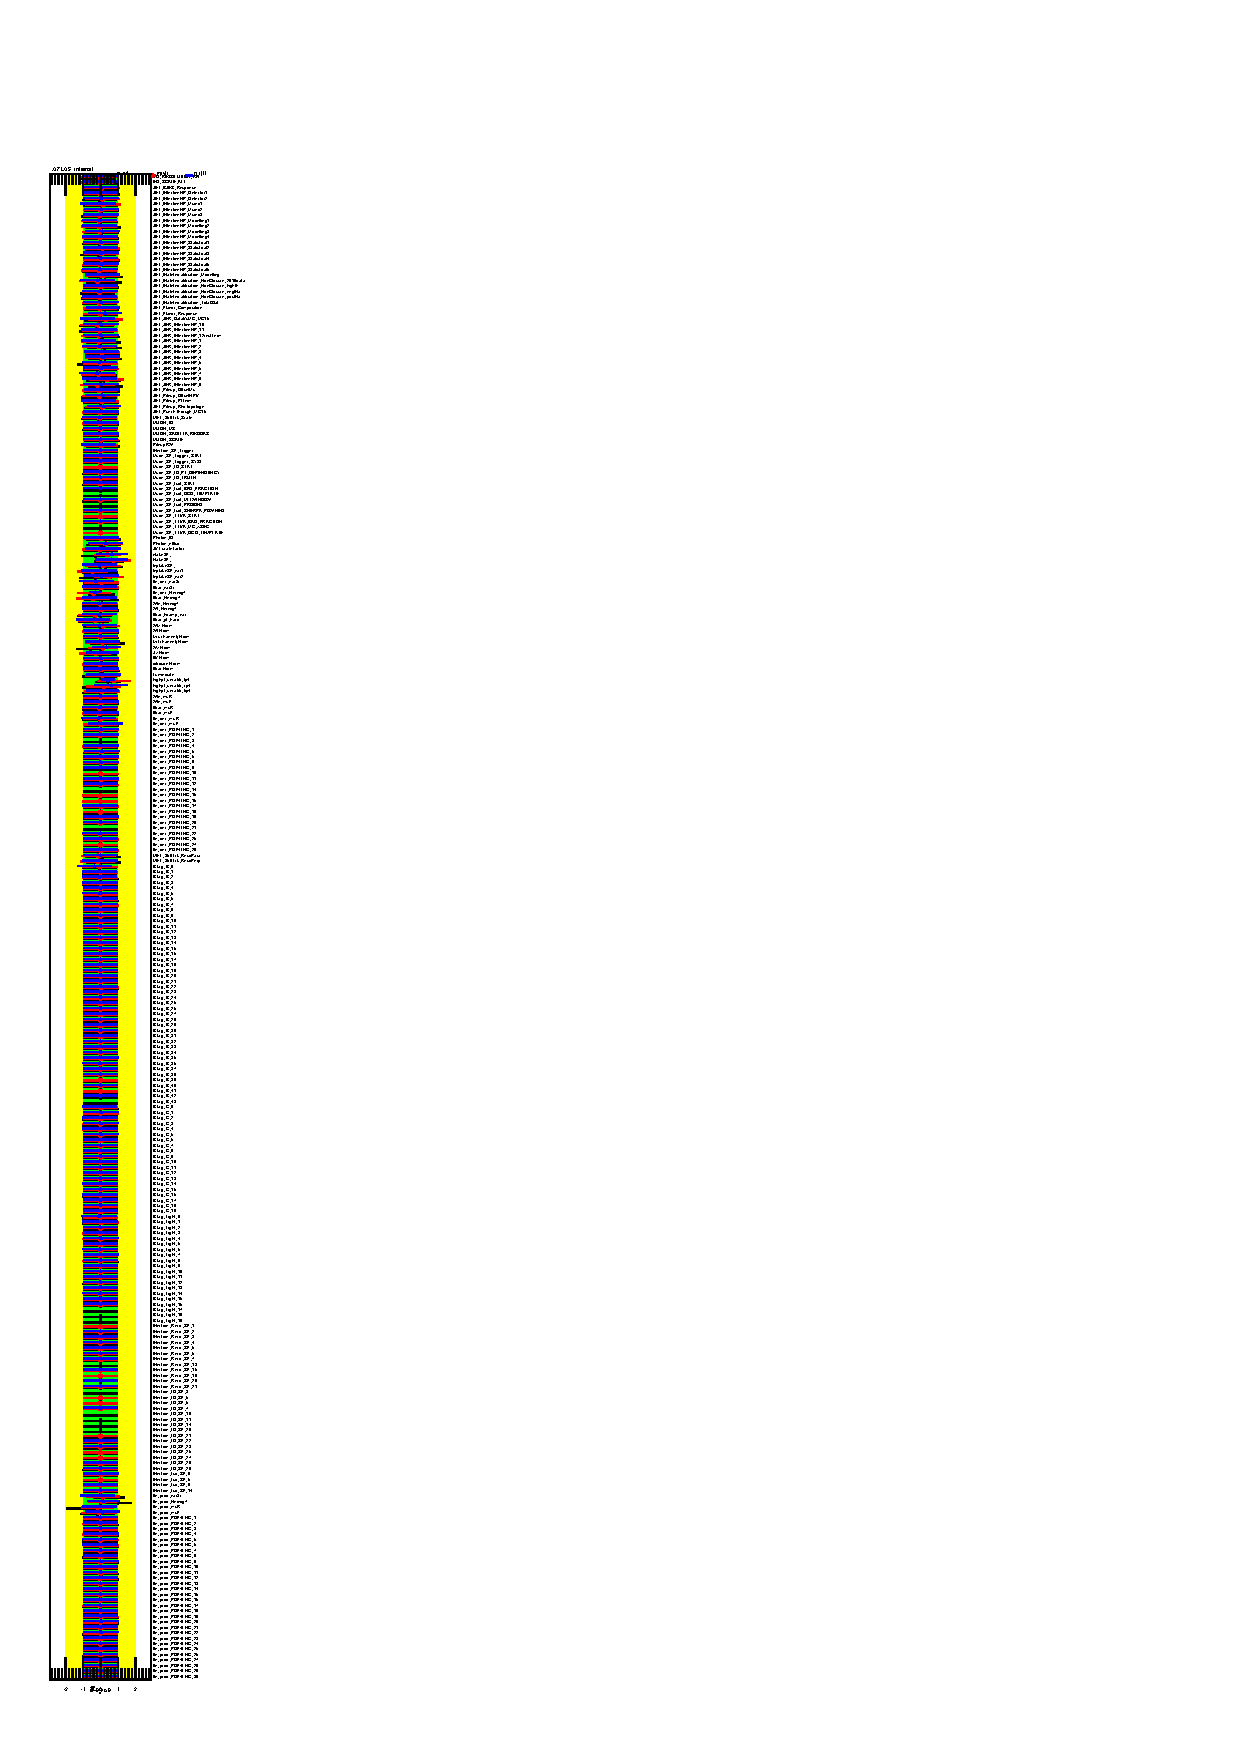
\includegraphics[width=0.40\textwidth, viewport=0 375 150 750, clip]{figures/diff_xsec/ljet_tty_prod_mu_blinded/compare_NP_pulls/compare_NP_dilep_fits_pt_ptj1_eta/NuisPar_comp.pdf}%
  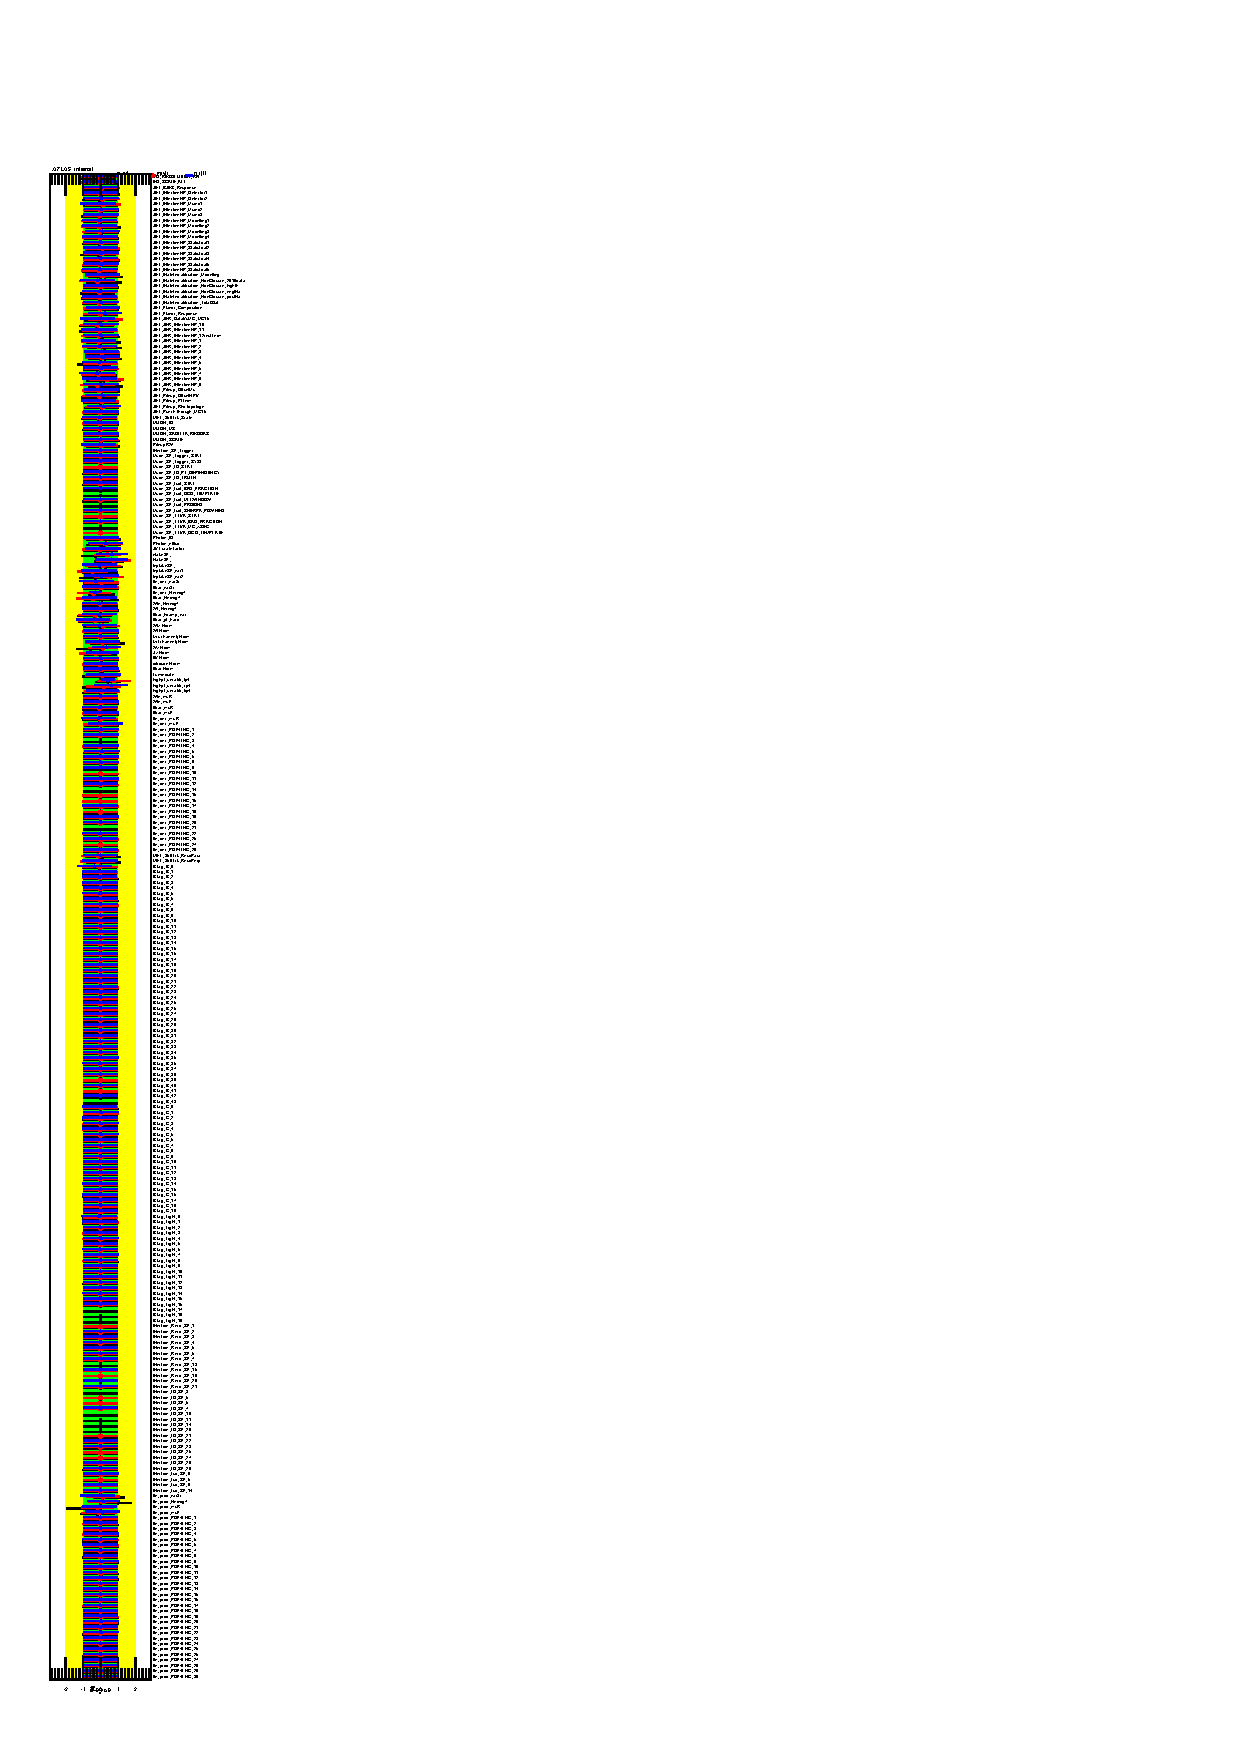
\includegraphics[width=0.40\textwidth, viewport=0 0 150 375, clip]{figures/diff_xsec/ljet_tty_prod_mu_blinded/compare_NP_pulls/compare_NP_dilep_fits_pt_ptj1_eta/NuisPar_comp.pdf}%
  \caption{Pull plots showing pulls and constraints for different observables in single-lepton channel for the \tty production measurement.}
  \label{fig:pull_plot_pt_tty_dec_free_ljet_mu_blinded}
\end{figure}

\begin{figure}[ht]
  \centering
  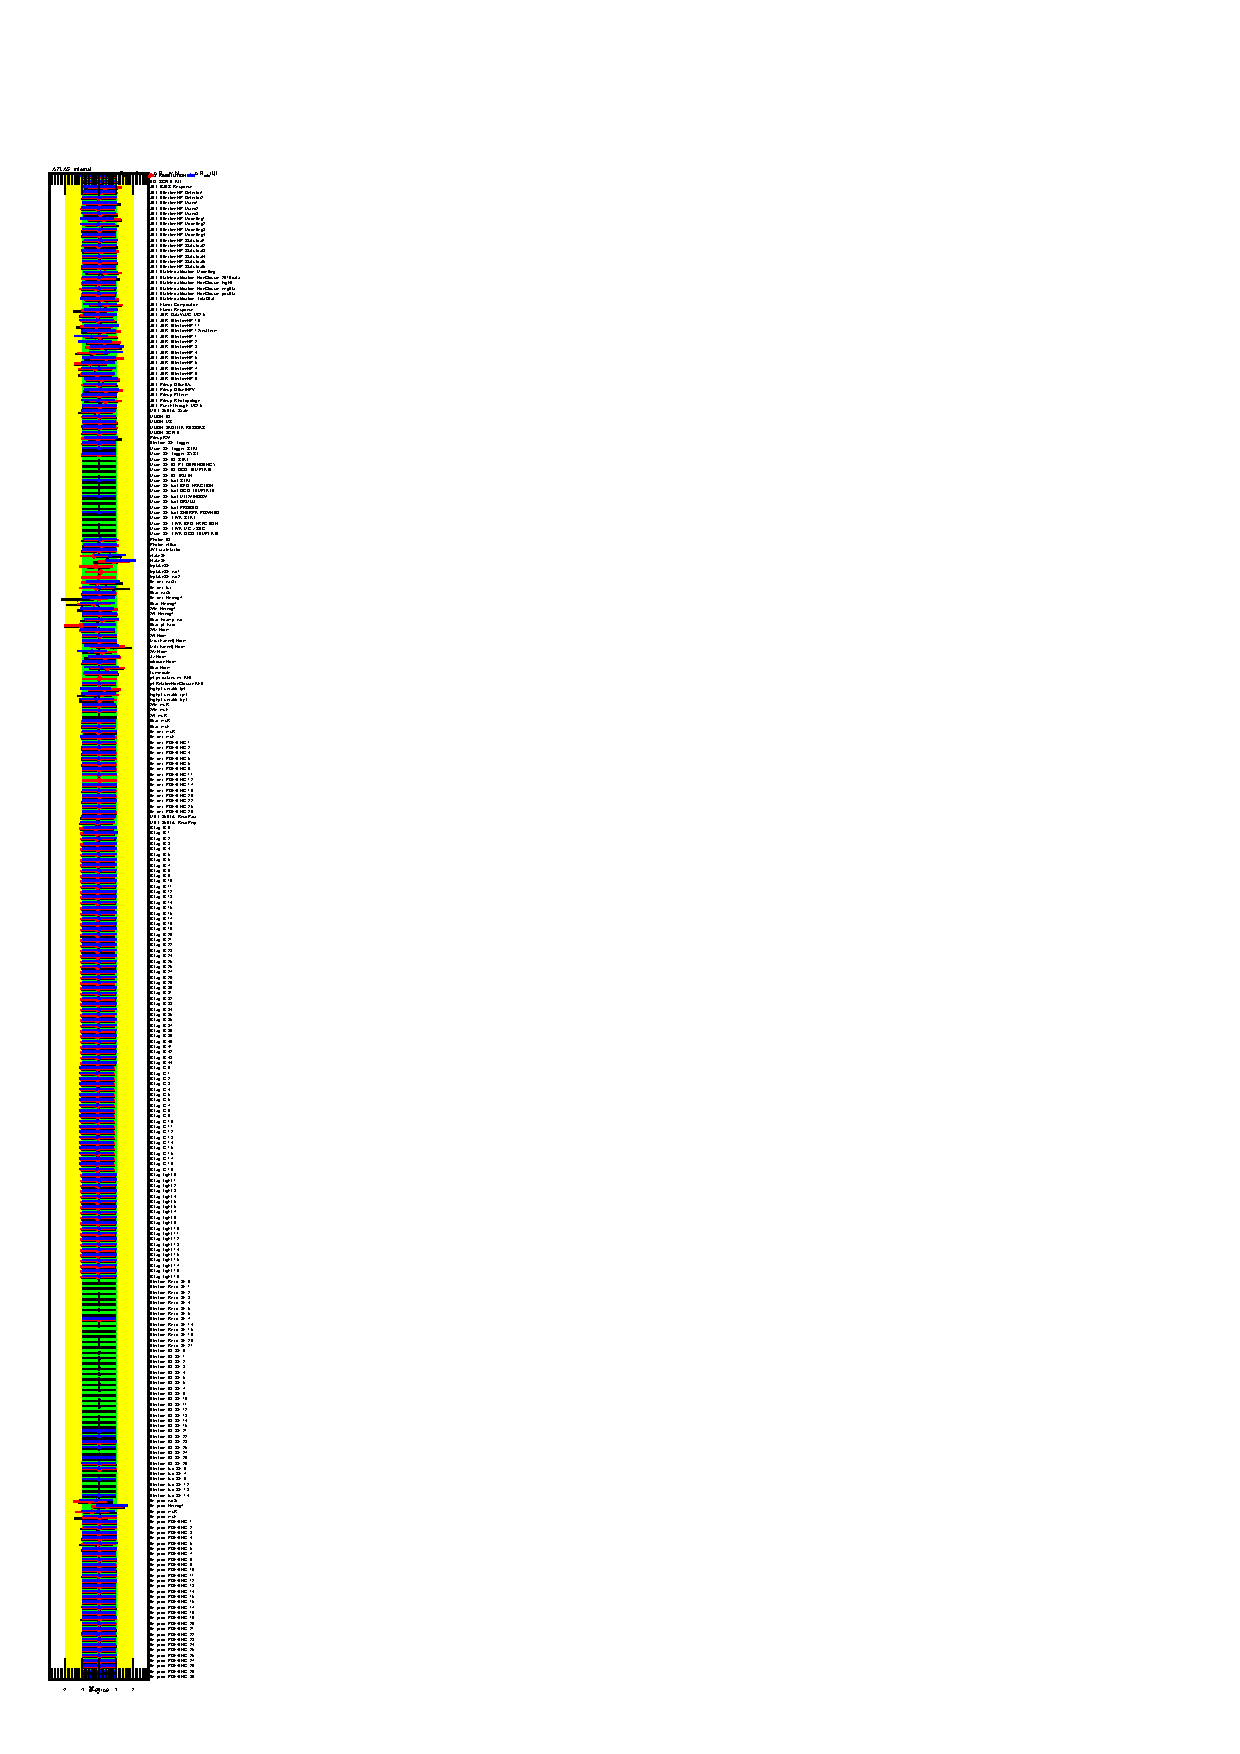
\includegraphics[width=0.40\textwidth, viewport=0 375 150 750, clip]{figures/diff_xsec/ljet_tty_prod_mu_blinded/compare_NP_pulls/compare_NP_dilep_fits_drphb_drlj_dr/NuisPar_comp.pdf}%
  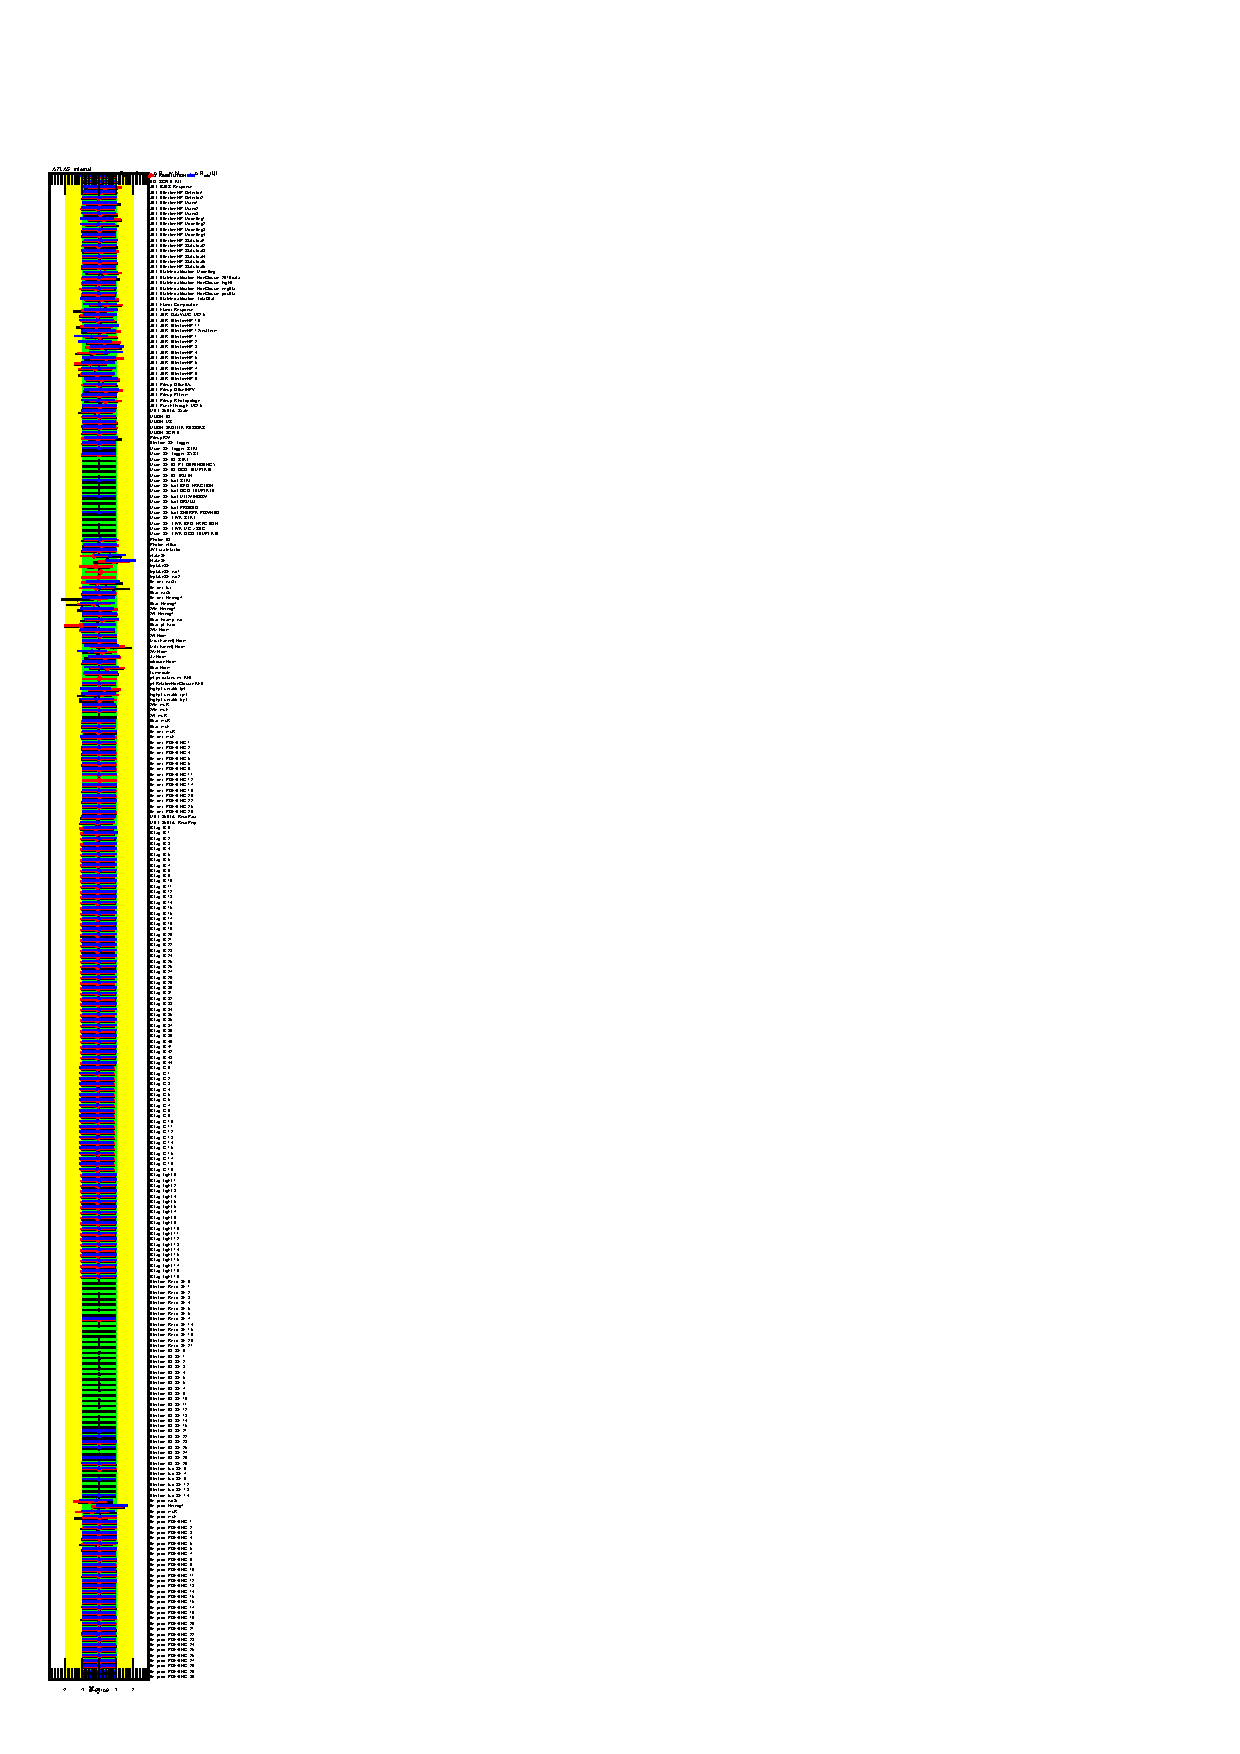
\includegraphics[width=0.40\textwidth, viewport=0 0 150 375, clip]{figures/diff_xsec/ljet_tty_prod_mu_blinded/compare_NP_pulls/compare_NP_dilep_fits_drphb_drlj_dr/NuisPar_comp.pdf}%
  \caption{Pull plots showing pulls and constraints for different observables in single-lepton channel for the \tty production measurement.}
  \label{fig:pull_plot_pt_tty_dec_free_ljet_mu_blinded}

\end{figure}


\begin{figure}[ht]
  \centering
  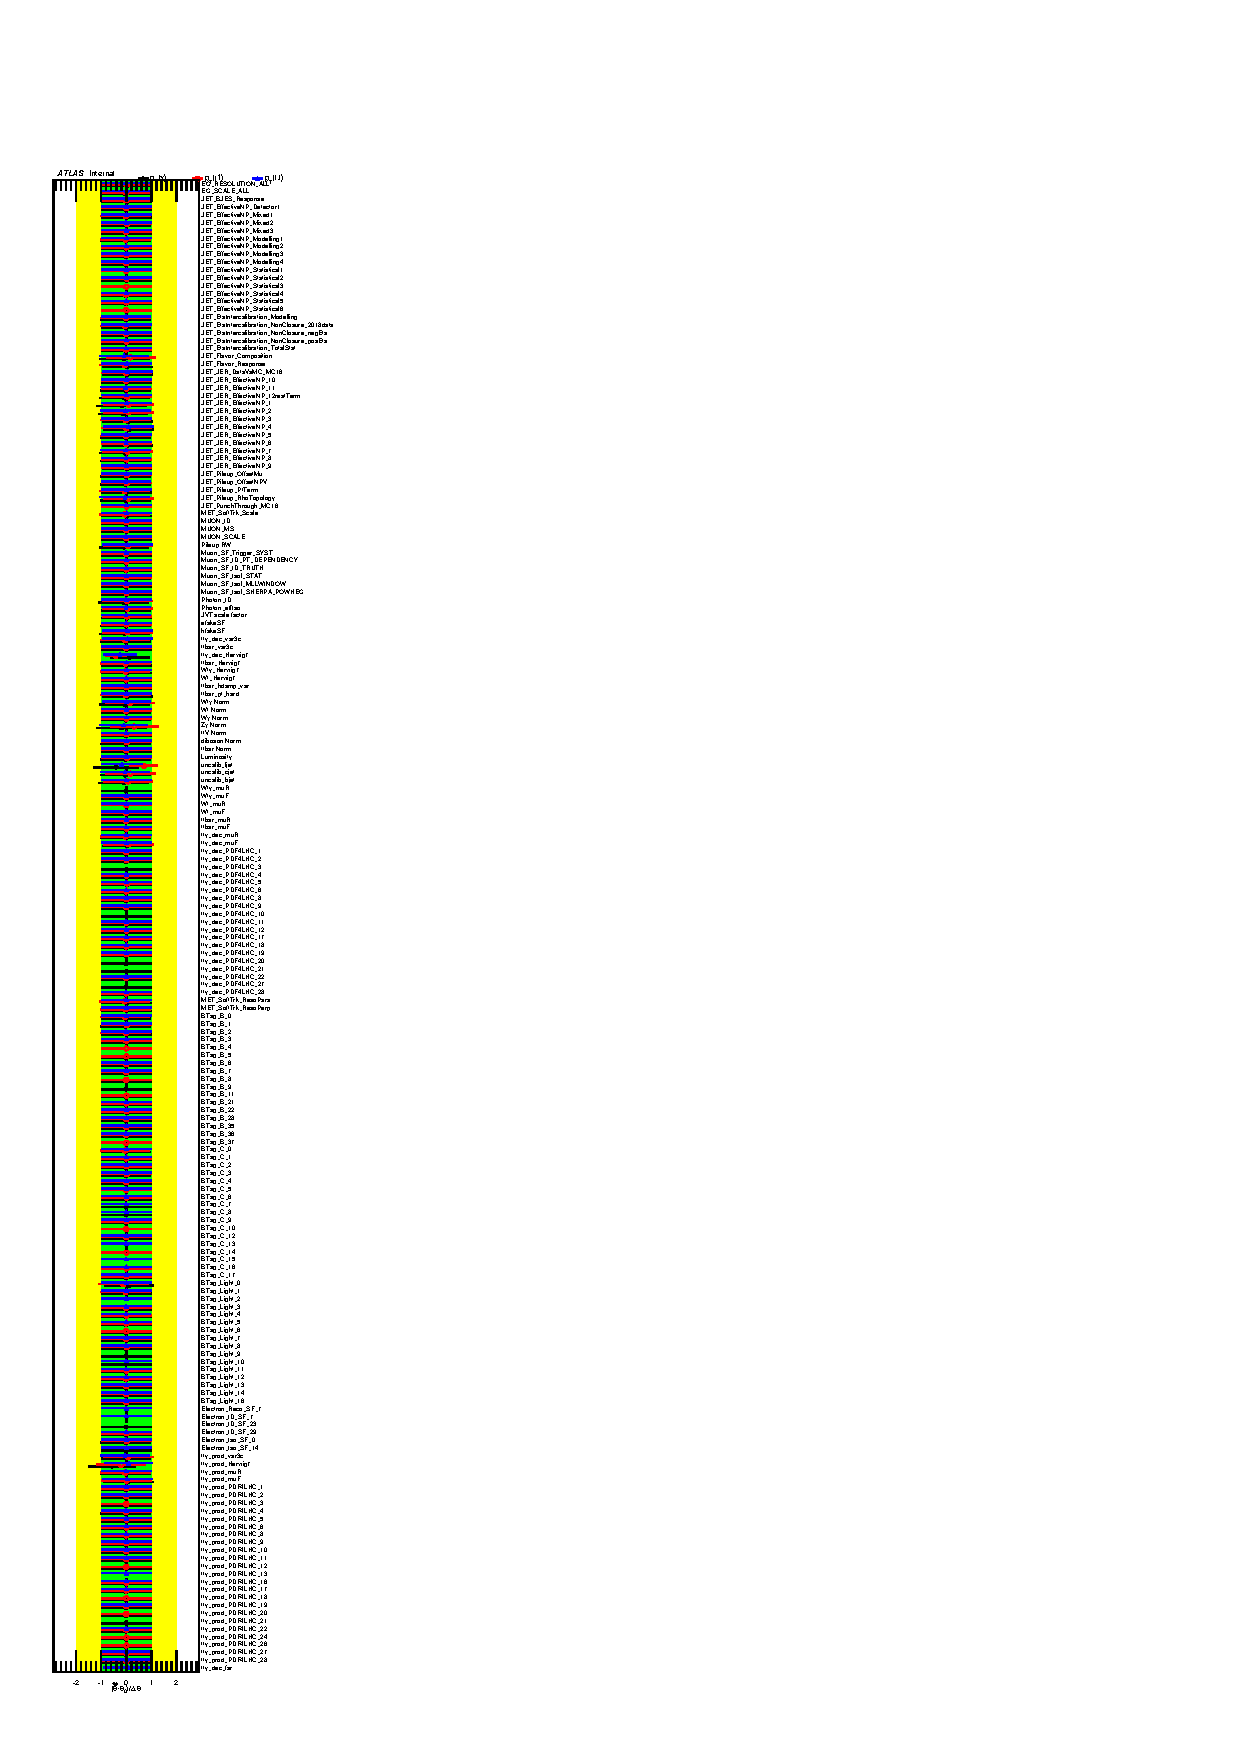
\includegraphics[width=0.35\textwidth]{figures/diff_xsec/dilep_tty_prod_mu_blinded/compare_NP_pulls/compare_NP_dilep_fits_pt_ptj1_ptll/NuisPar_comp.pdf}%
  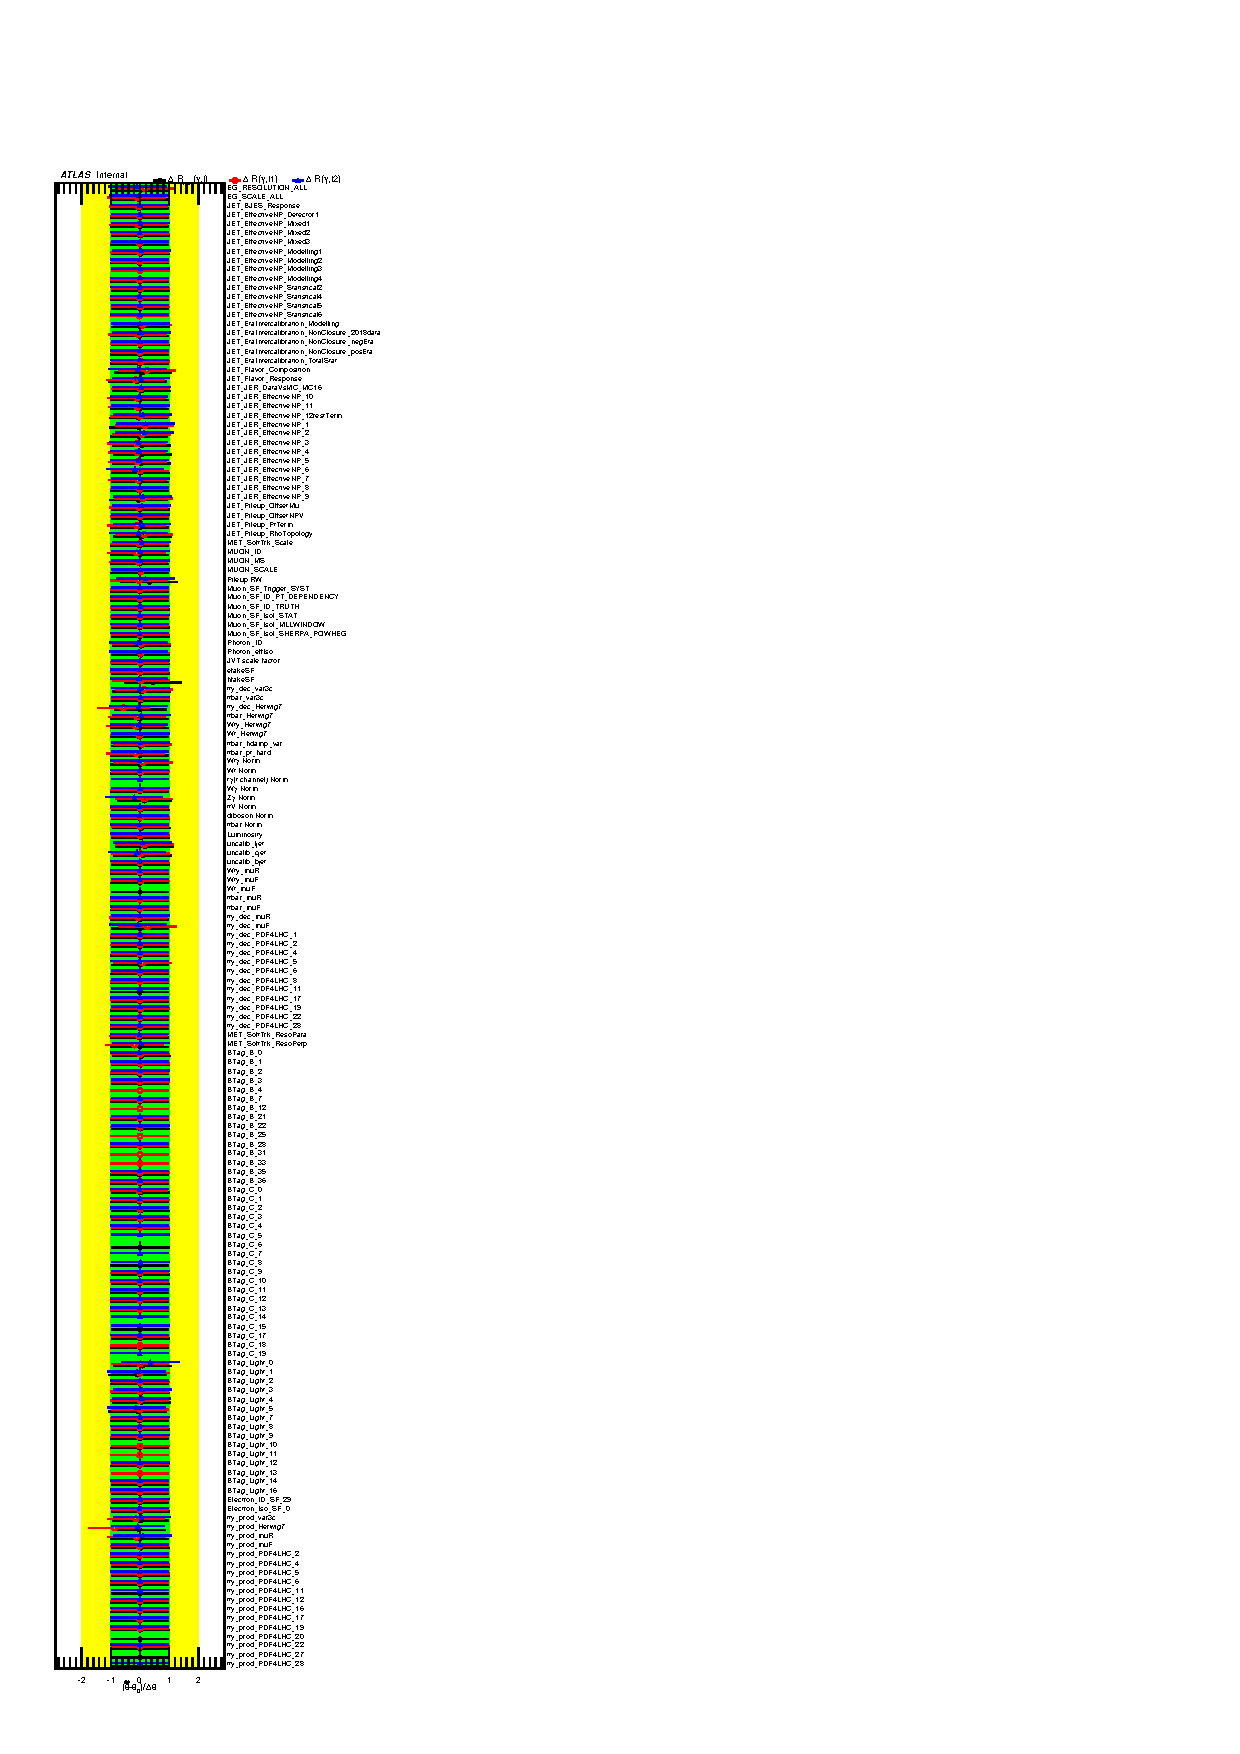
\includegraphics[width=0.35\textwidth]{figures/diff_xsec/dilep_tty_prod_mu_blinded/compare_NP_pulls/compare_NP_dilep_fits_dr_dr1_dr2/NuisPar_comp.pdf}%
  \caption{Pull plots showing pulls and constraints for different observables in dilepton channel for the \tty production measurement.}
  \label{fig:pull_plot_pt_tty_dec_free_dilep_mu_blinded_1}
\end{figure}
\FloatBarrier

\begin{figure}[ht]
  \centering
  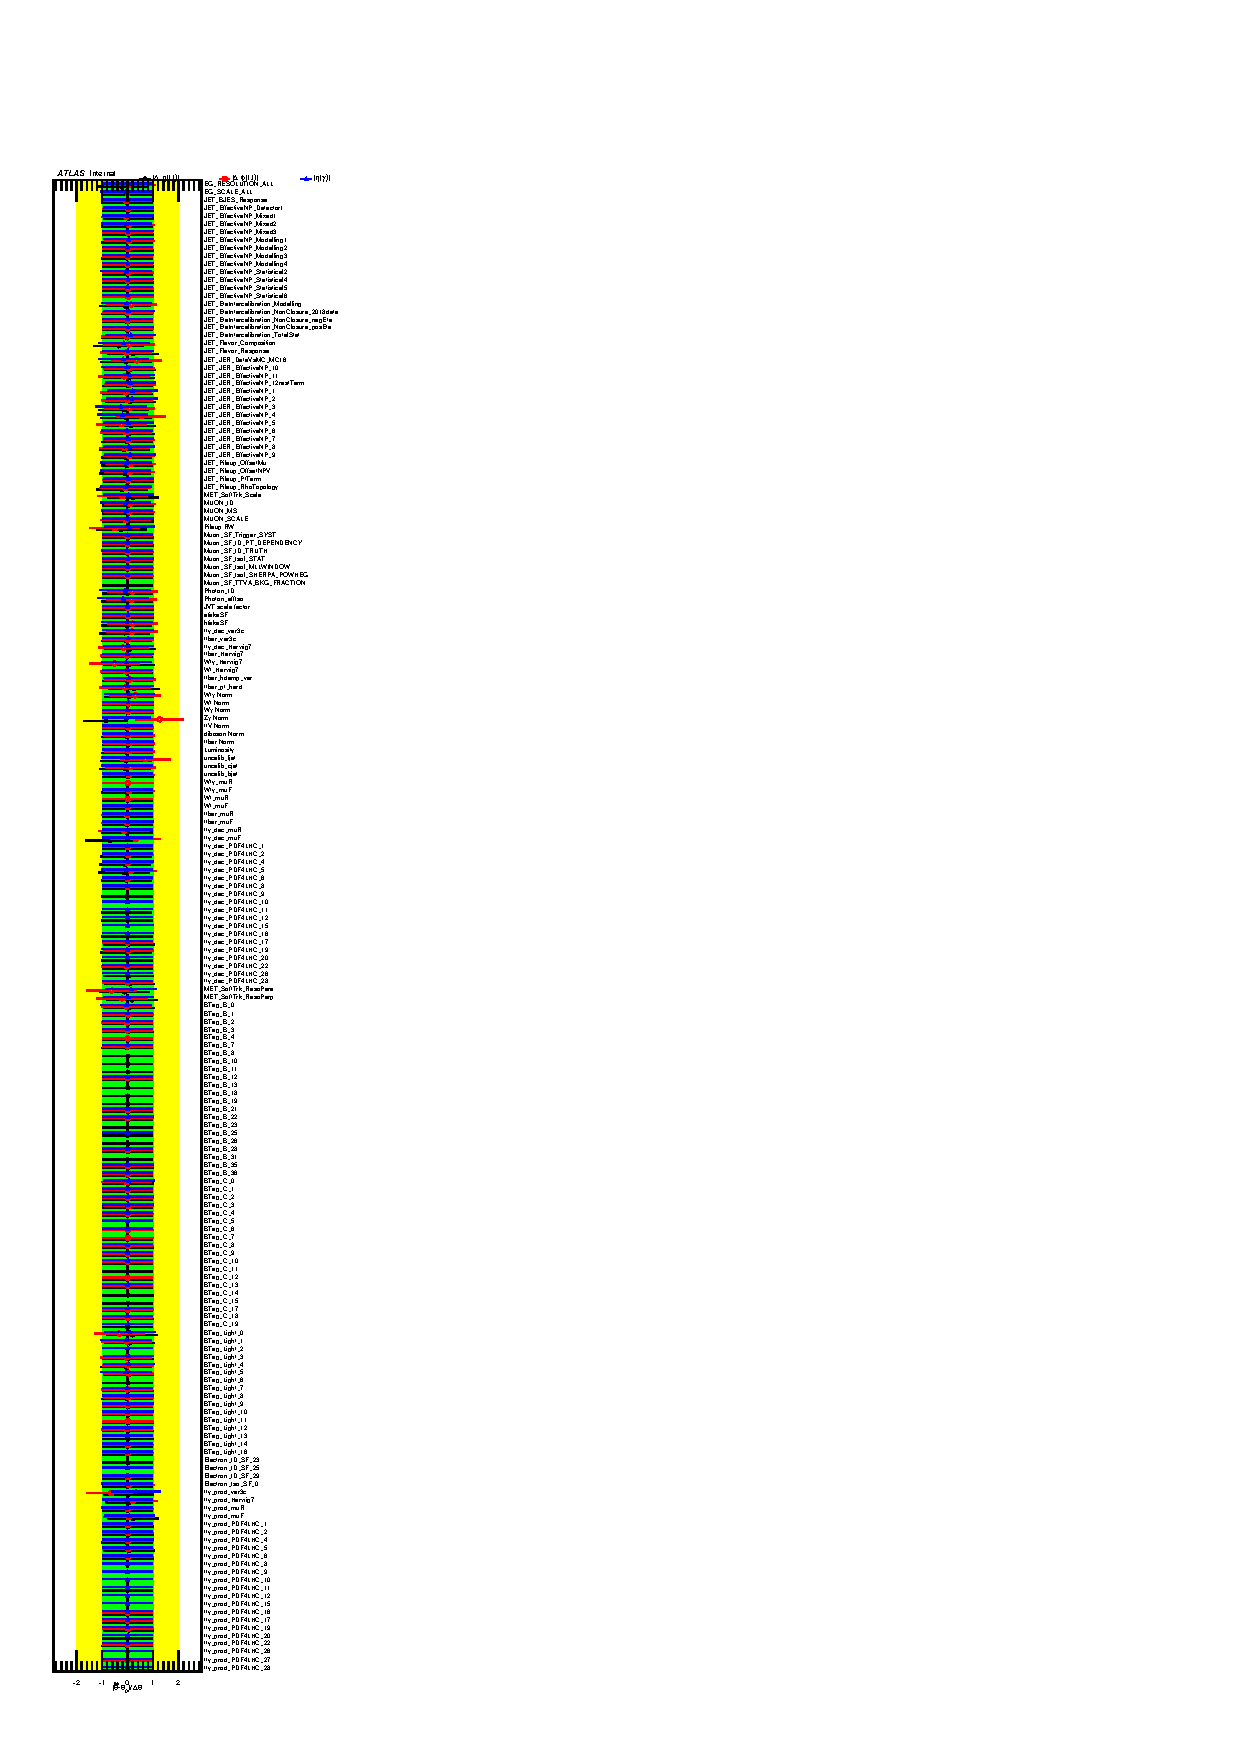
\includegraphics[width=0.35\textwidth]{figures/diff_xsec/dilep_tty_prod_mu_blinded/compare_NP_pulls/compare_NP_dilep_fits_detall_dphill_eta/NuisPar_comp.pdf}%
  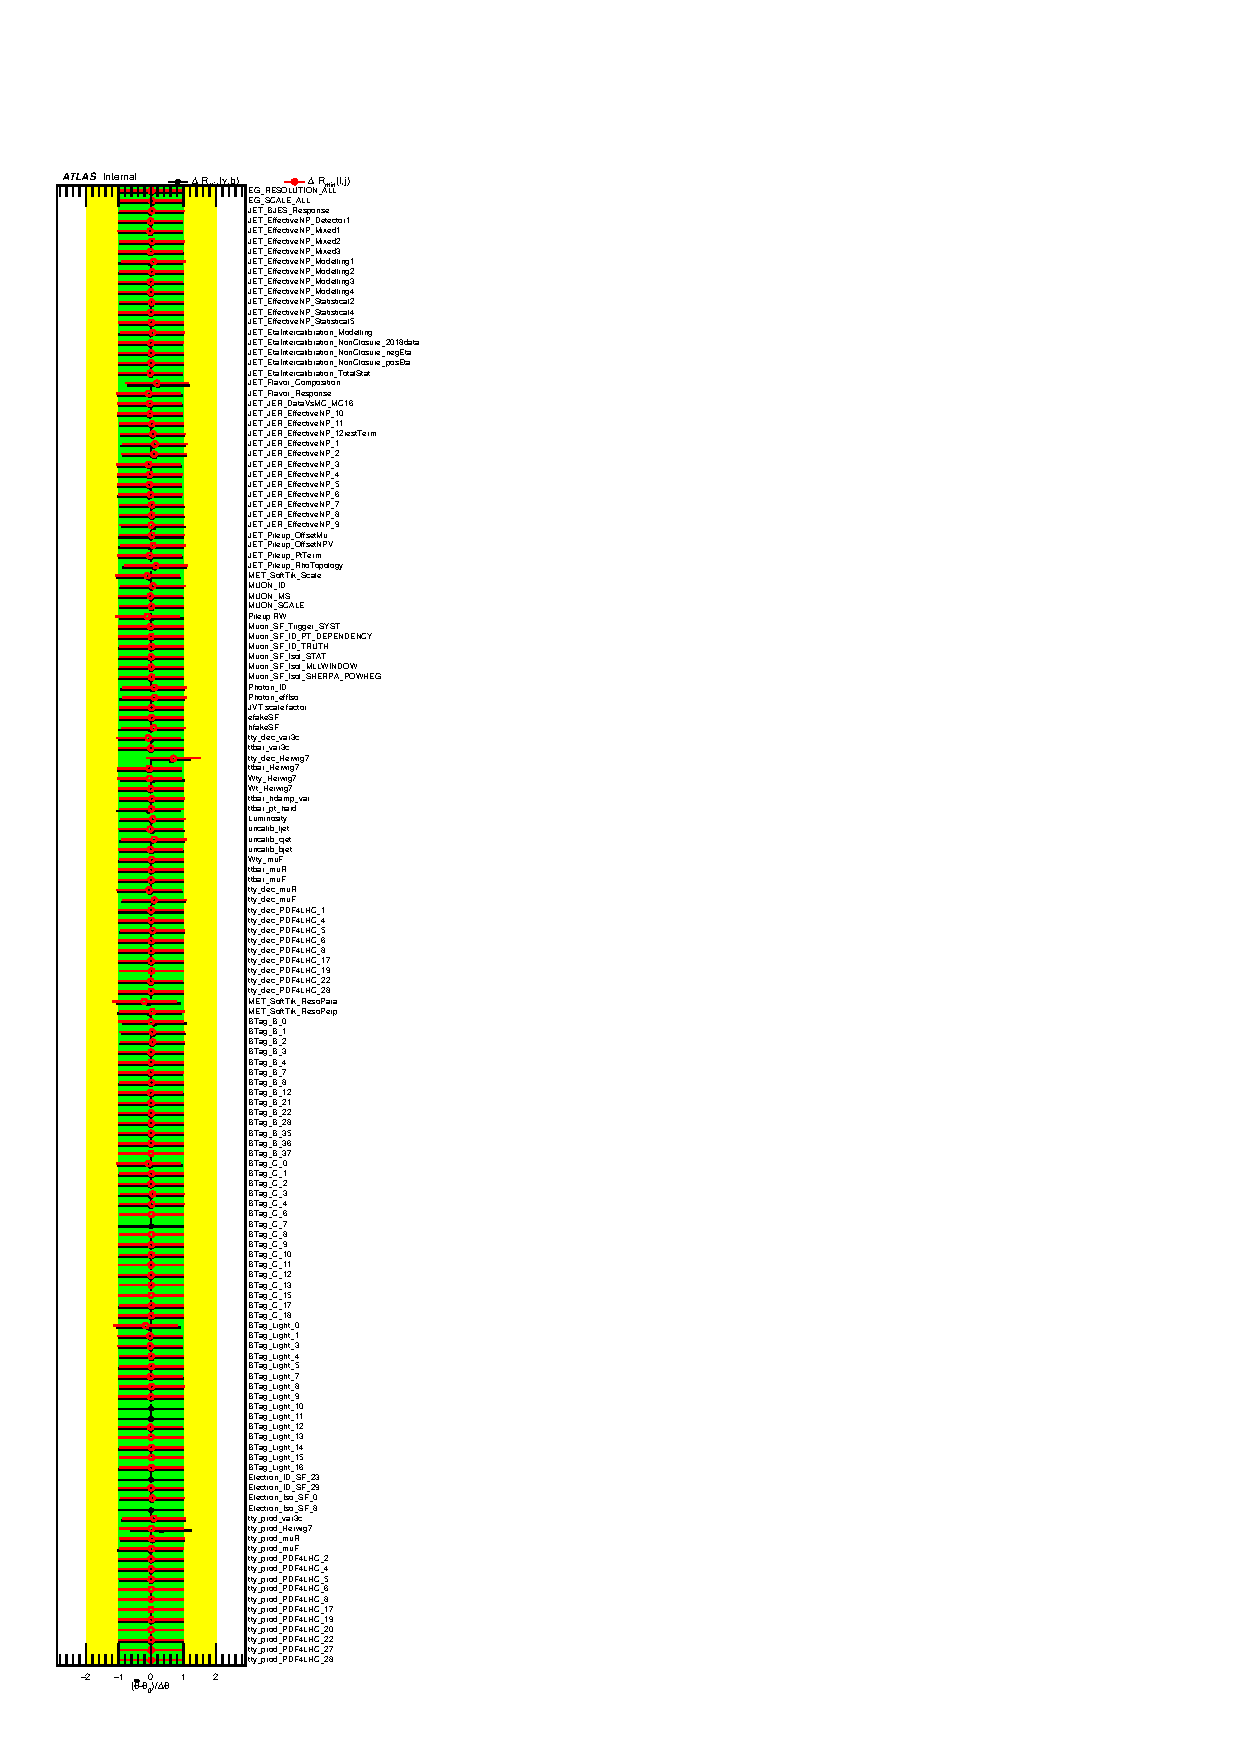
\includegraphics[width=0.35\textwidth]{figures/diff_xsec/dilep_tty_prod_mu_blinded/compare_NP_pulls/compare_NP_dilep_fits_drphb_drlj/NuisPar_comp.pdf}%
  \caption{Pull plots showing pulls and constraints for different observables in dilepton channel for the \tty production measurement.}
  \label{fig:pull_plot_pt_tty_dec_free_dilep_mu_blinded_2}
\end{figure}
\FloatBarrier

\begin{figure}[ht]
  \centering
  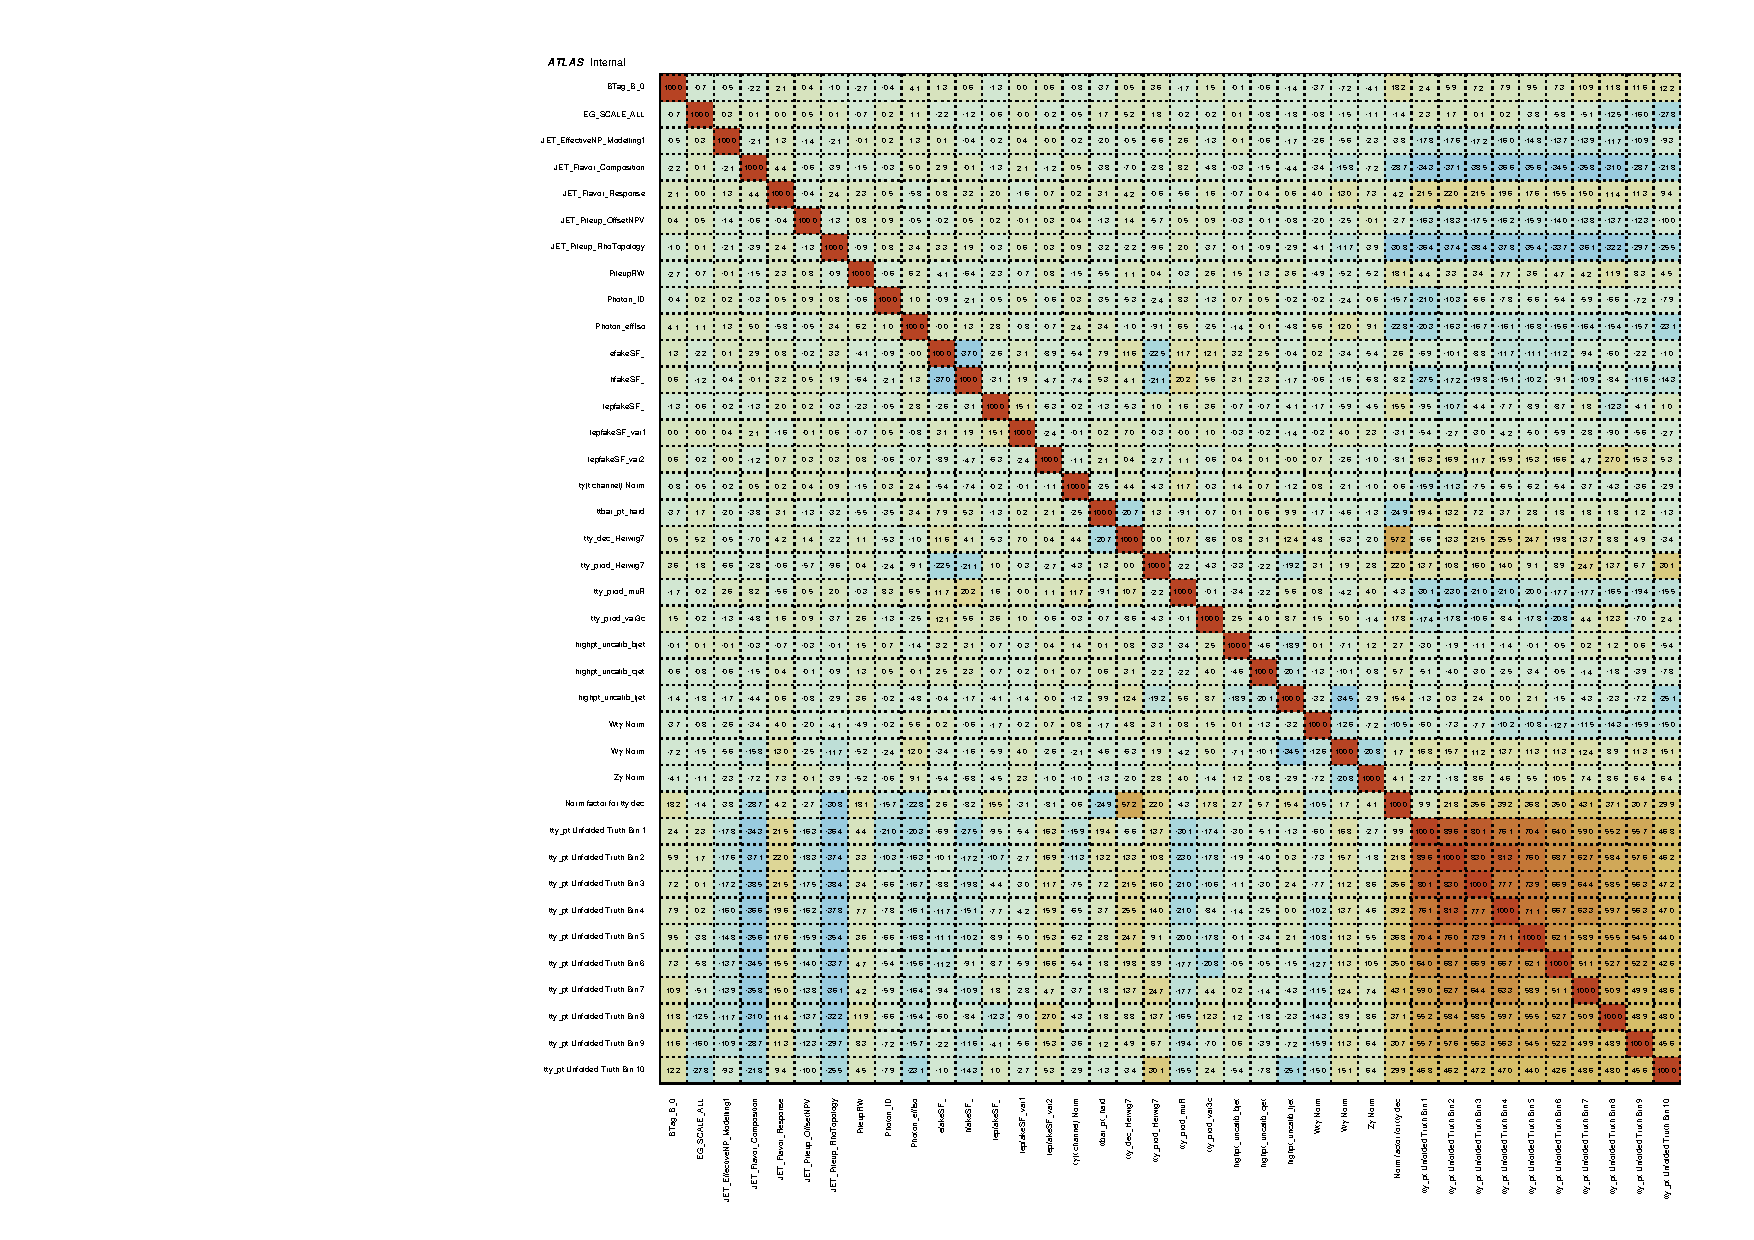
\includegraphics[width=0.8\textwidth]{figures/diff_xsec/ljet_tty_prod_mu_blinded/correlations/tty1l_pt_all_syst/CorrMatrix.pdf}
  \caption{The correlation among NPs and POIs for the measurement of the \ptgamma distribution in single-lepton channel for the \tty production measurement.}
  \label{fig:NP_corr_ljet_mu_blinded}
\end{figure}
\FloatBarrier


\begin{figure}[ht]
  \centering
  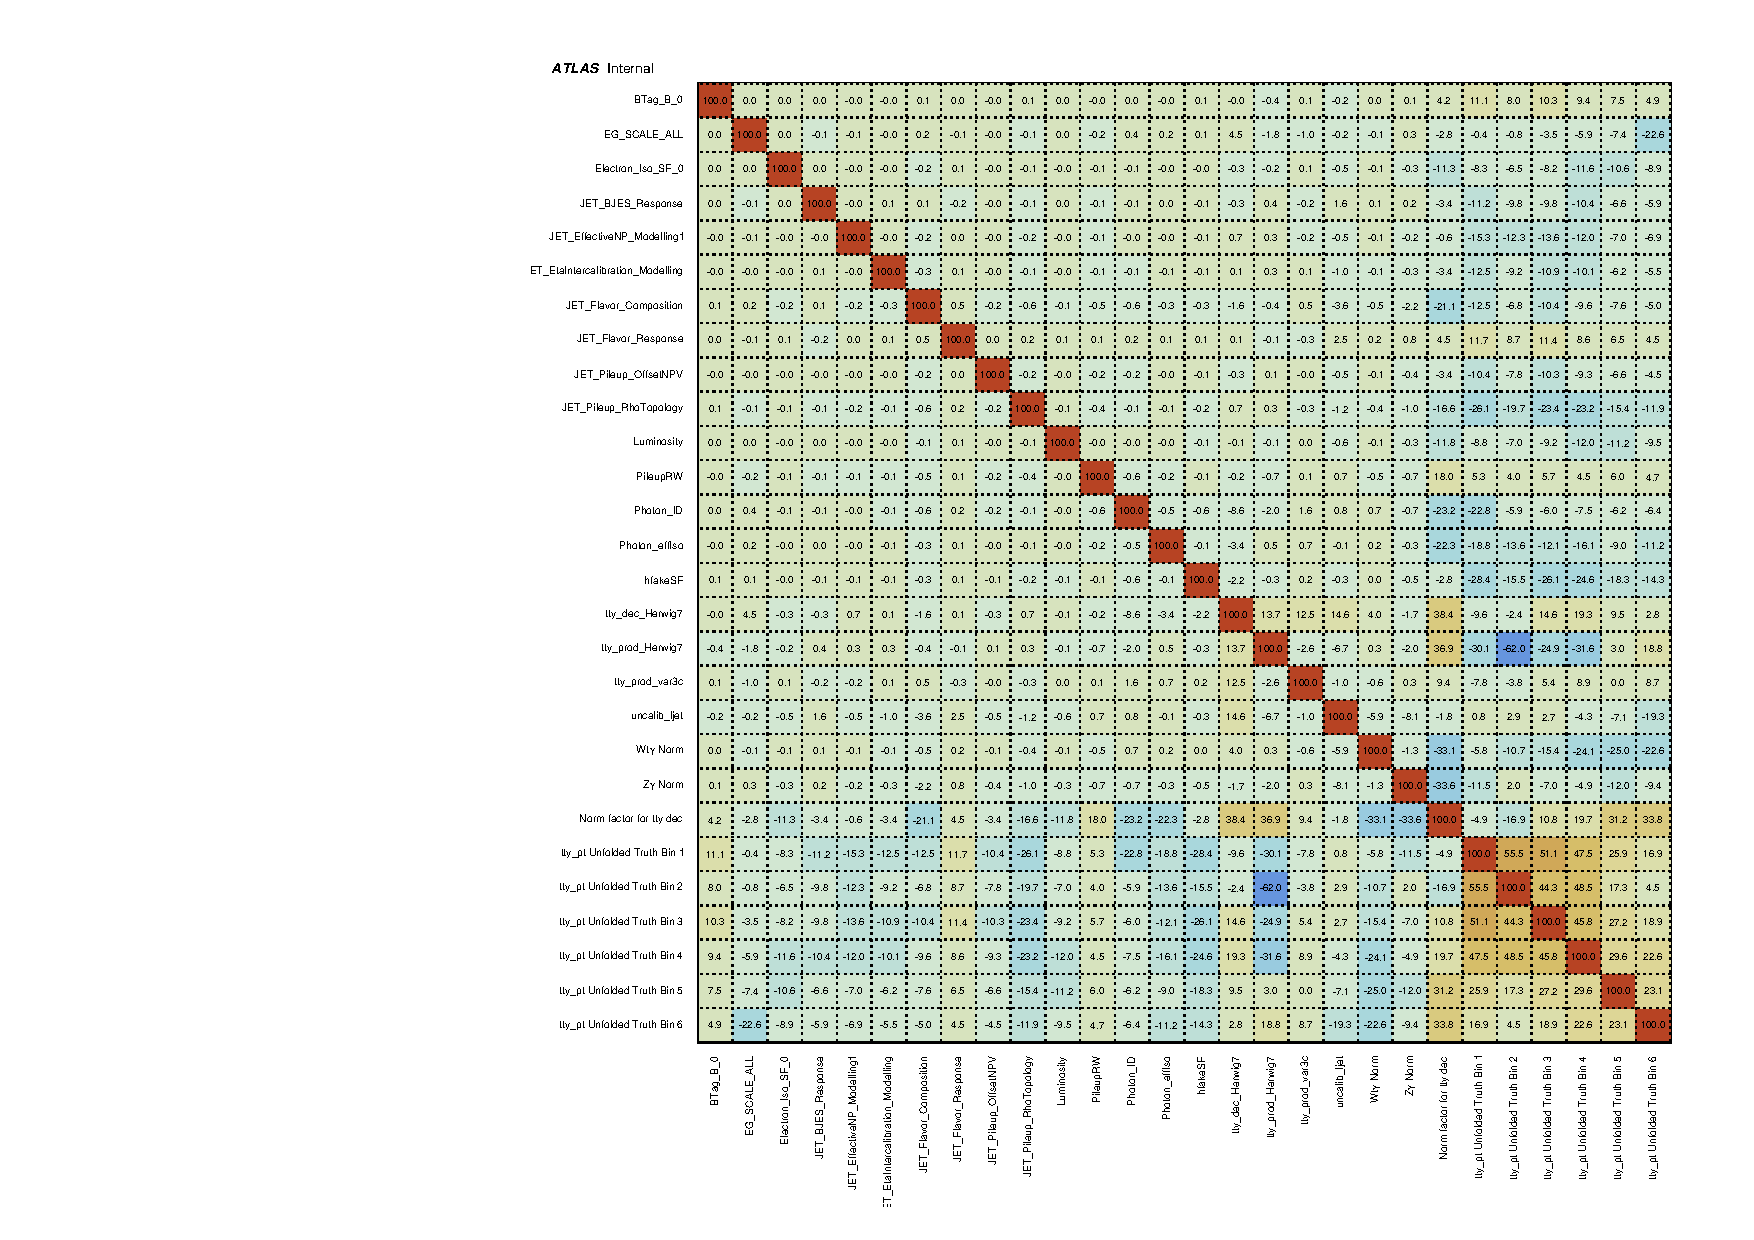
\includegraphics[width=0.8\textwidth]{figures/diff_xsec/dilep_tty_prod_mu_blinded/correlations/tty2l_pt_all_syst/CorrMatrix.pdf}
  \caption{The correlation among NPs and POIs for the measurement of the \ptgamma distribution in dilepton channel for the \tty production measurement.}
  \label{fig:NP_corr_dilep_mu_blinded}
\end{figure}
\FloatBarrier

%%%%%%%%%%%% RANKING %%%%%%%%%%%%%%%%%%%

\begin{figure}[ht]
  \centering
  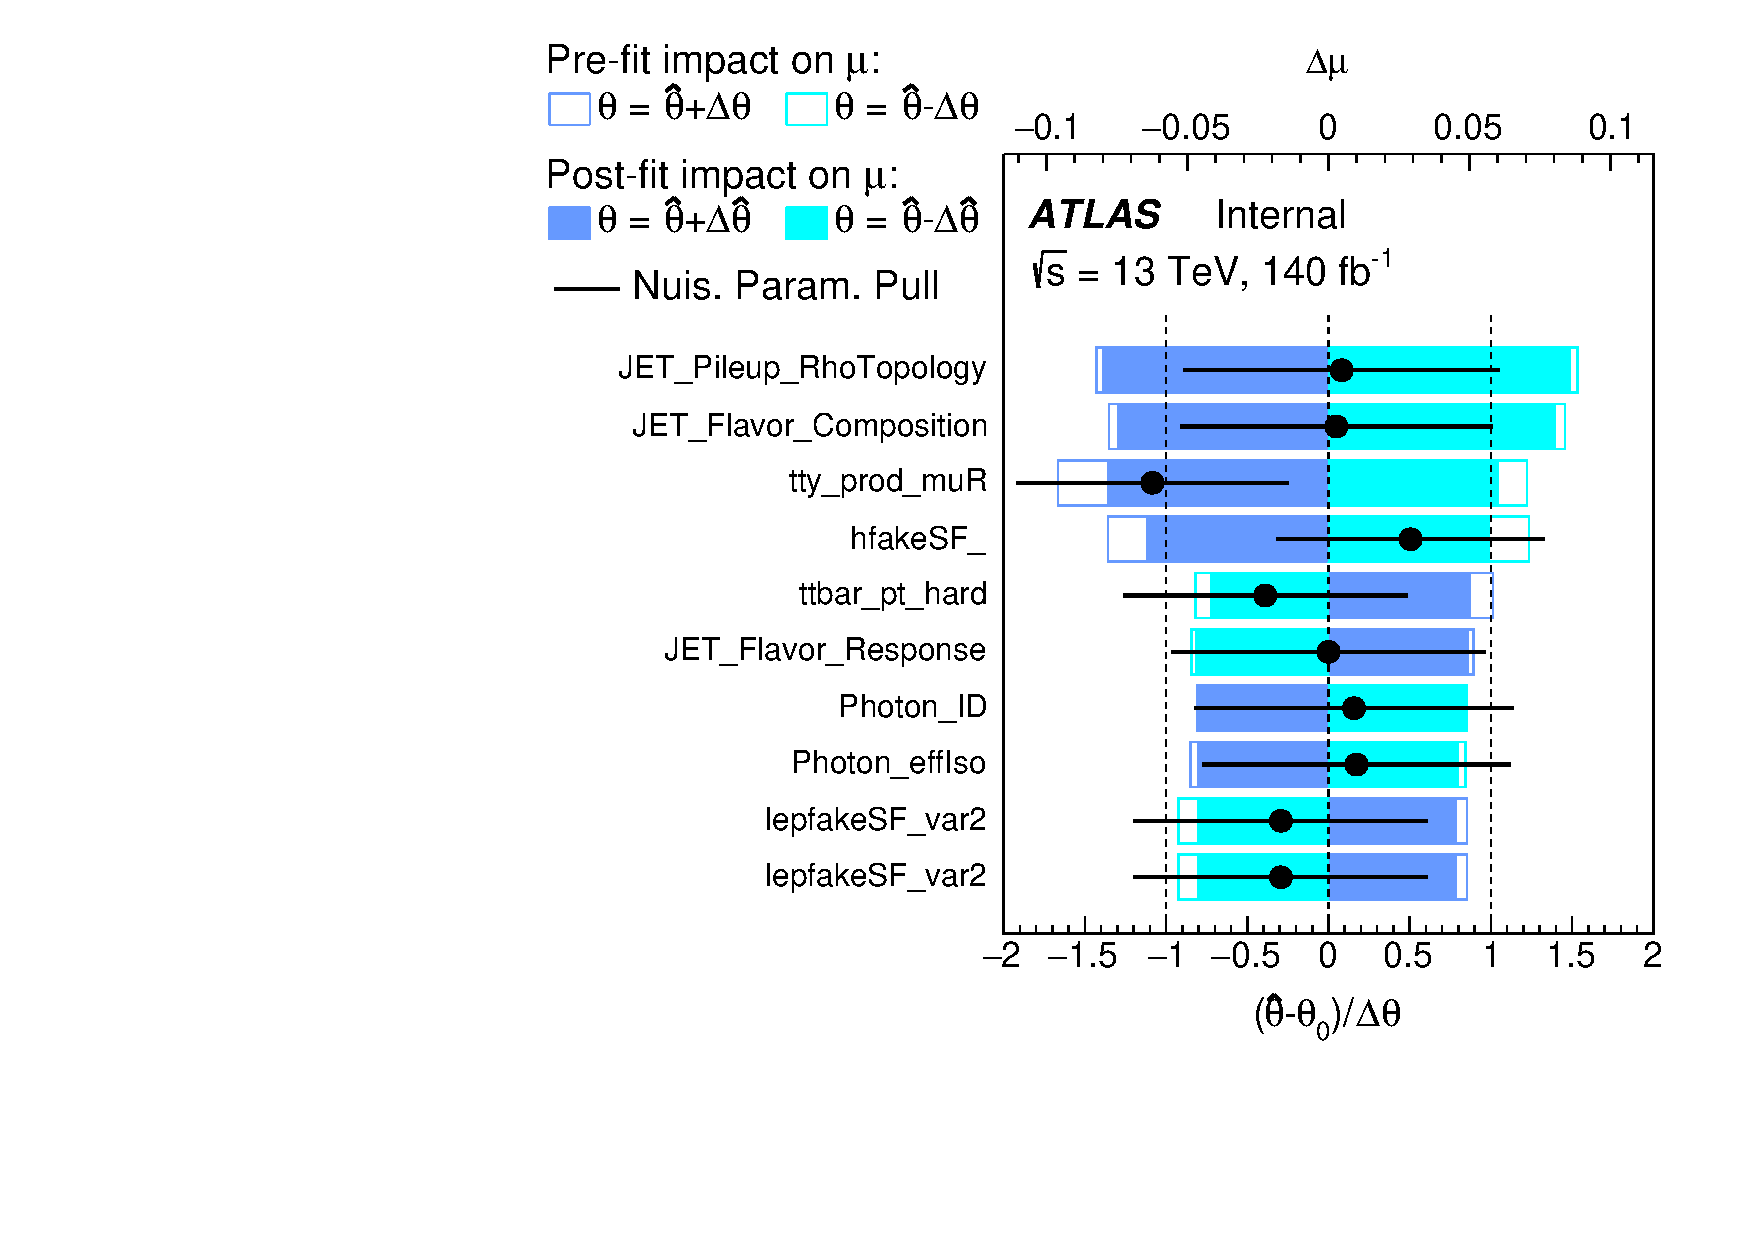
\includegraphics[width=0.33\textwidth]{figures/diff_xsec/ljet_tty_prod_mu_blinded/Ranking/tty1l_pt_all_syst/Ranking_tty_pt_Bin_001_mu.pdf}%
  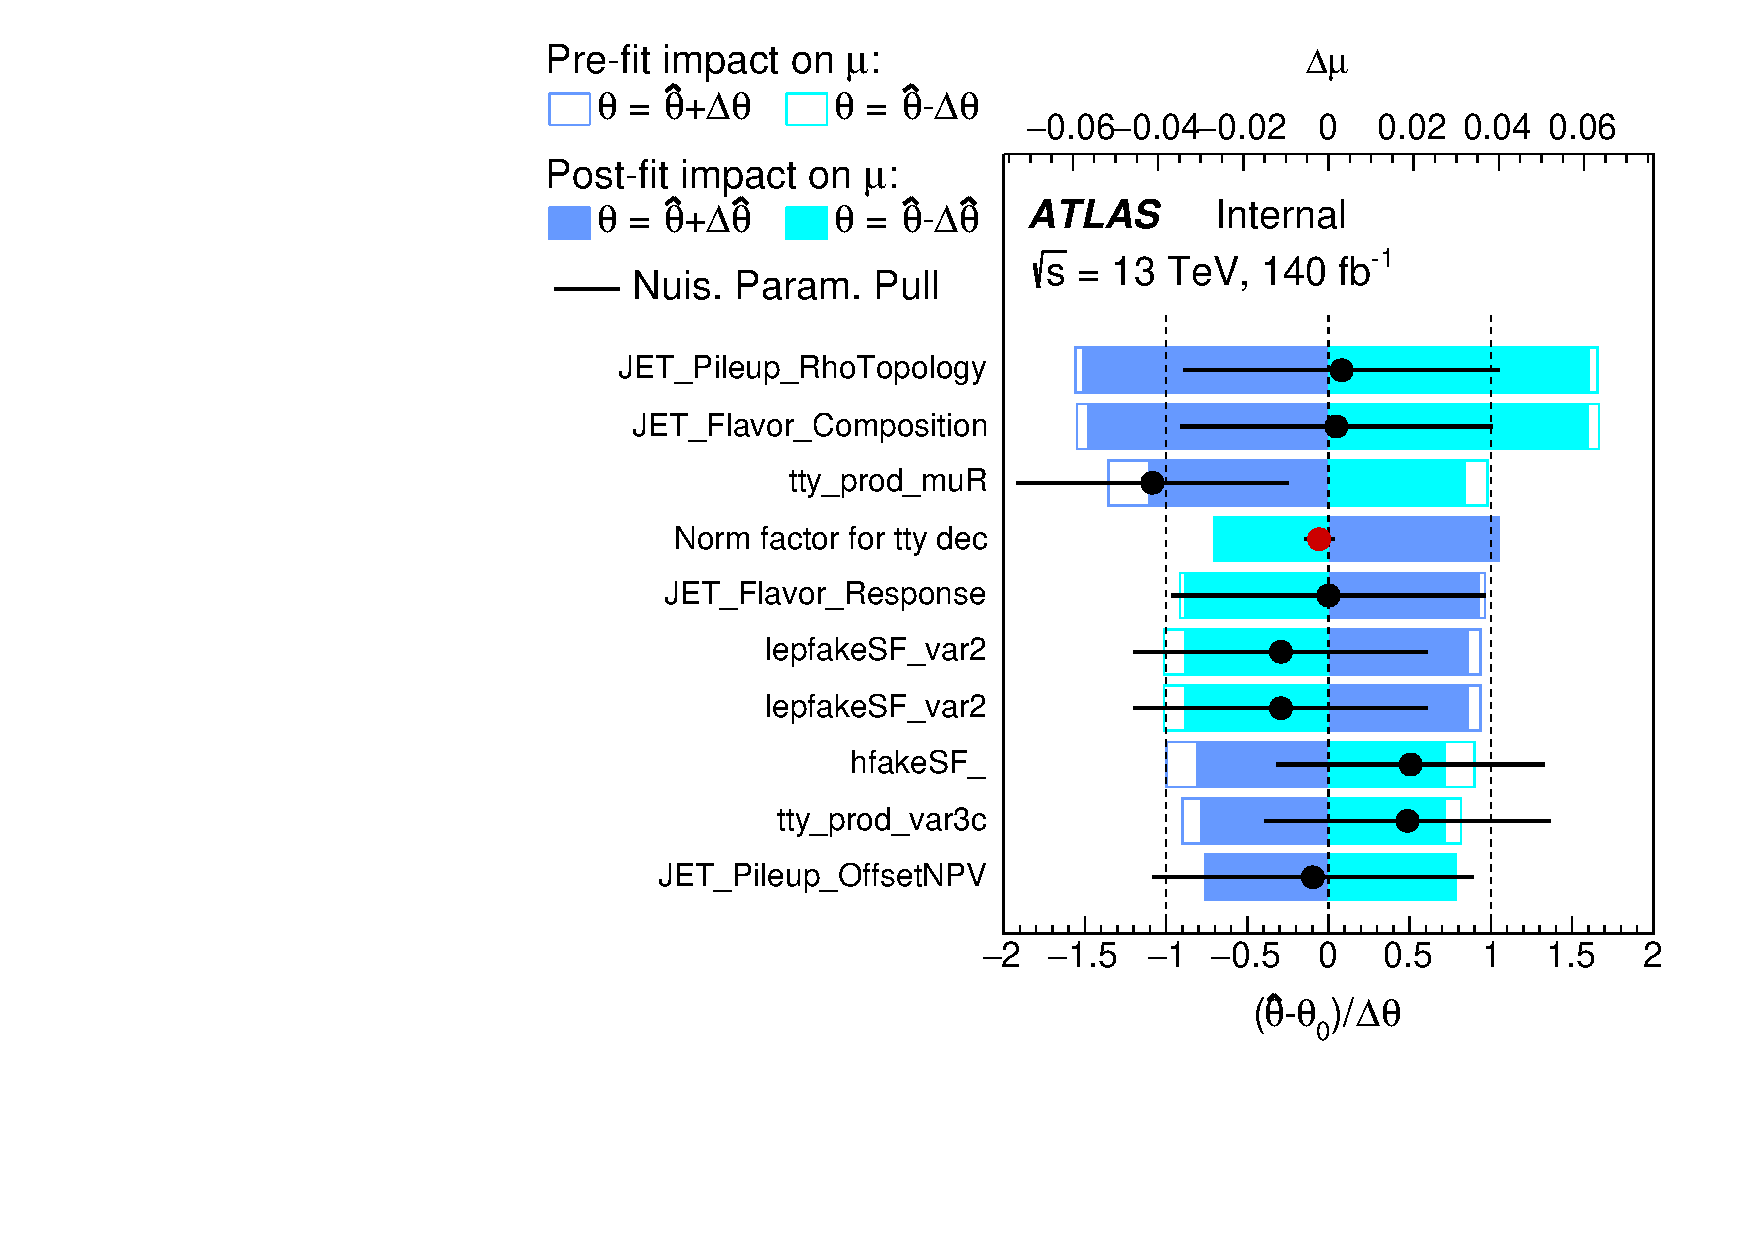
\includegraphics[width=0.33\textwidth]{figures/diff_xsec/ljet_tty_prod_mu_blinded/Ranking/tty1l_pt_all_syst/Ranking_tty_pt_Bin_002_mu.pdf}%
  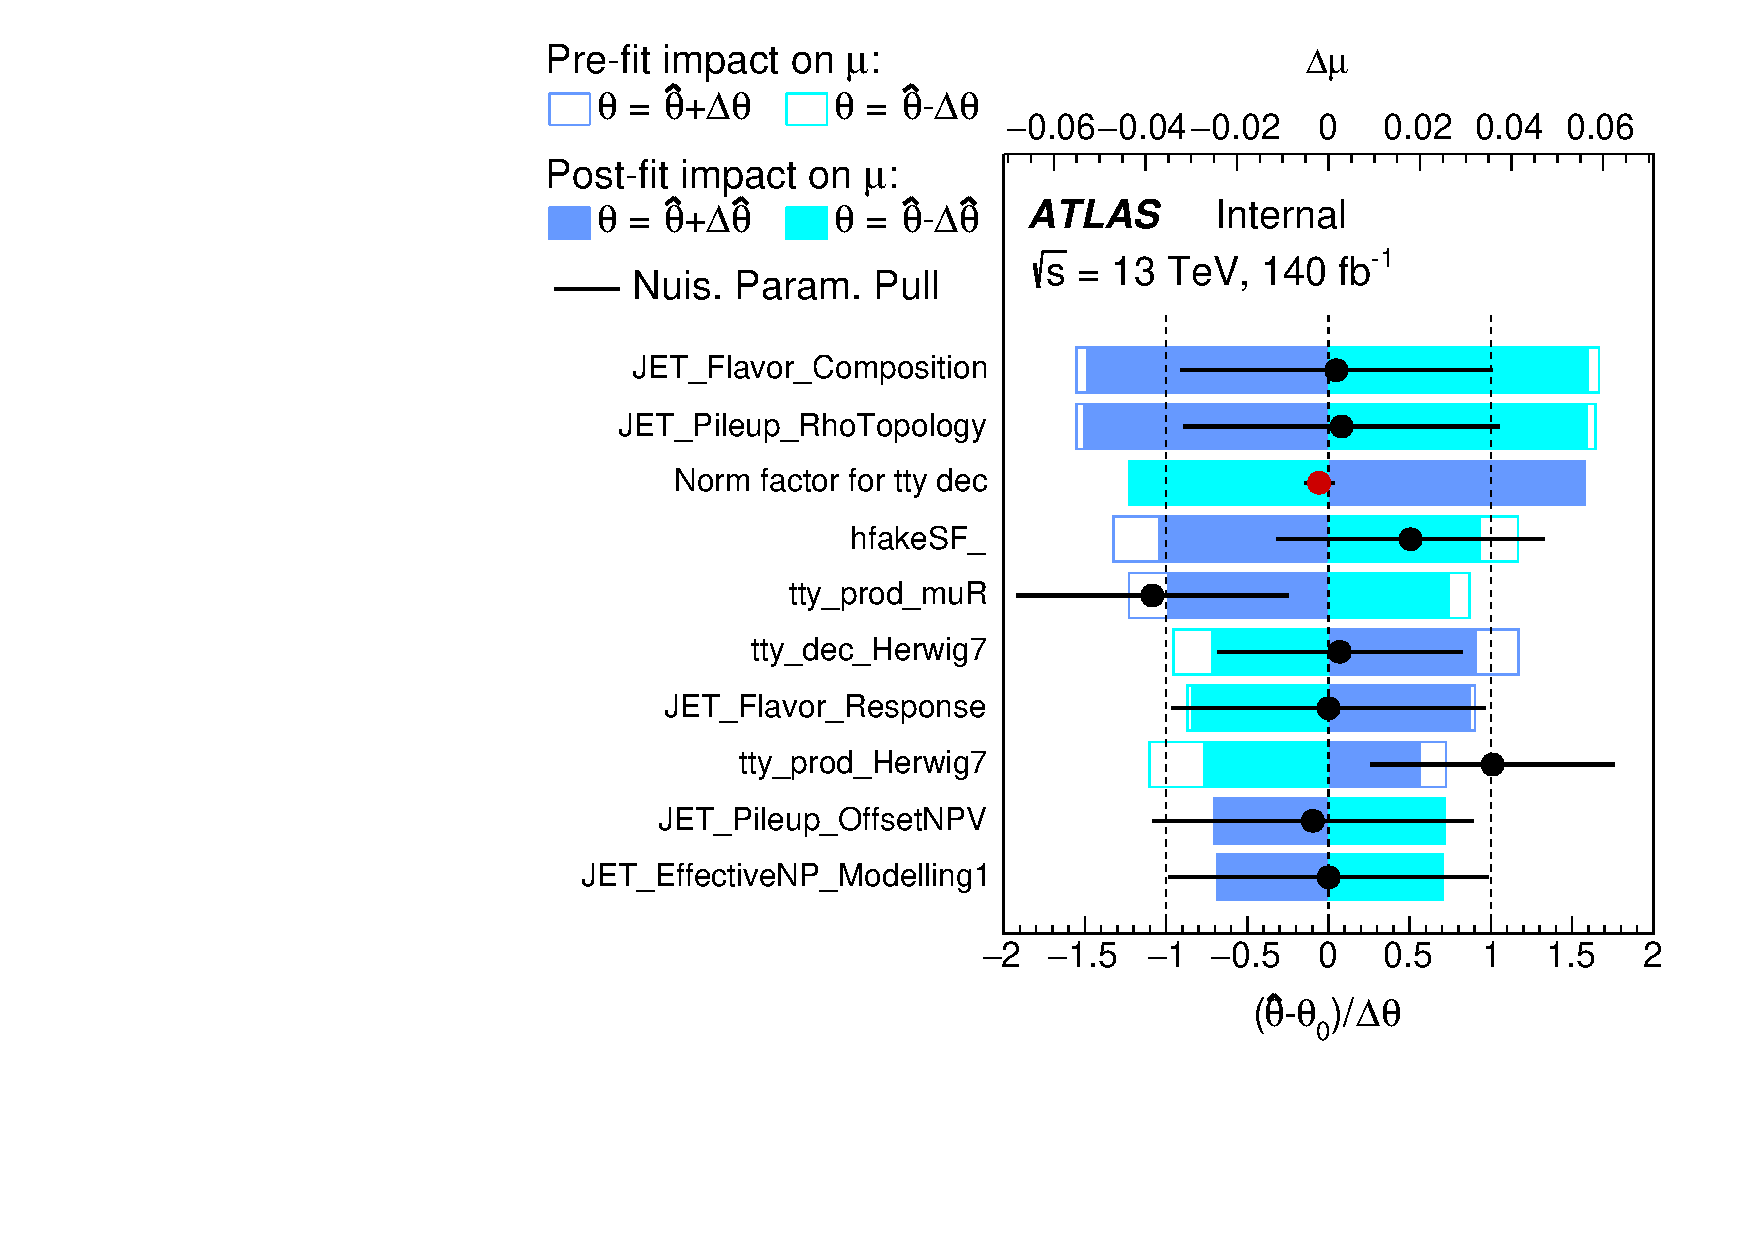
\includegraphics[width=0.33\textwidth]{figures/diff_xsec/ljet_tty_prod_mu_blinded/Ranking/tty1l_pt_all_syst/Ranking_tty_pt_Bin_003_mu.pdf}\\
  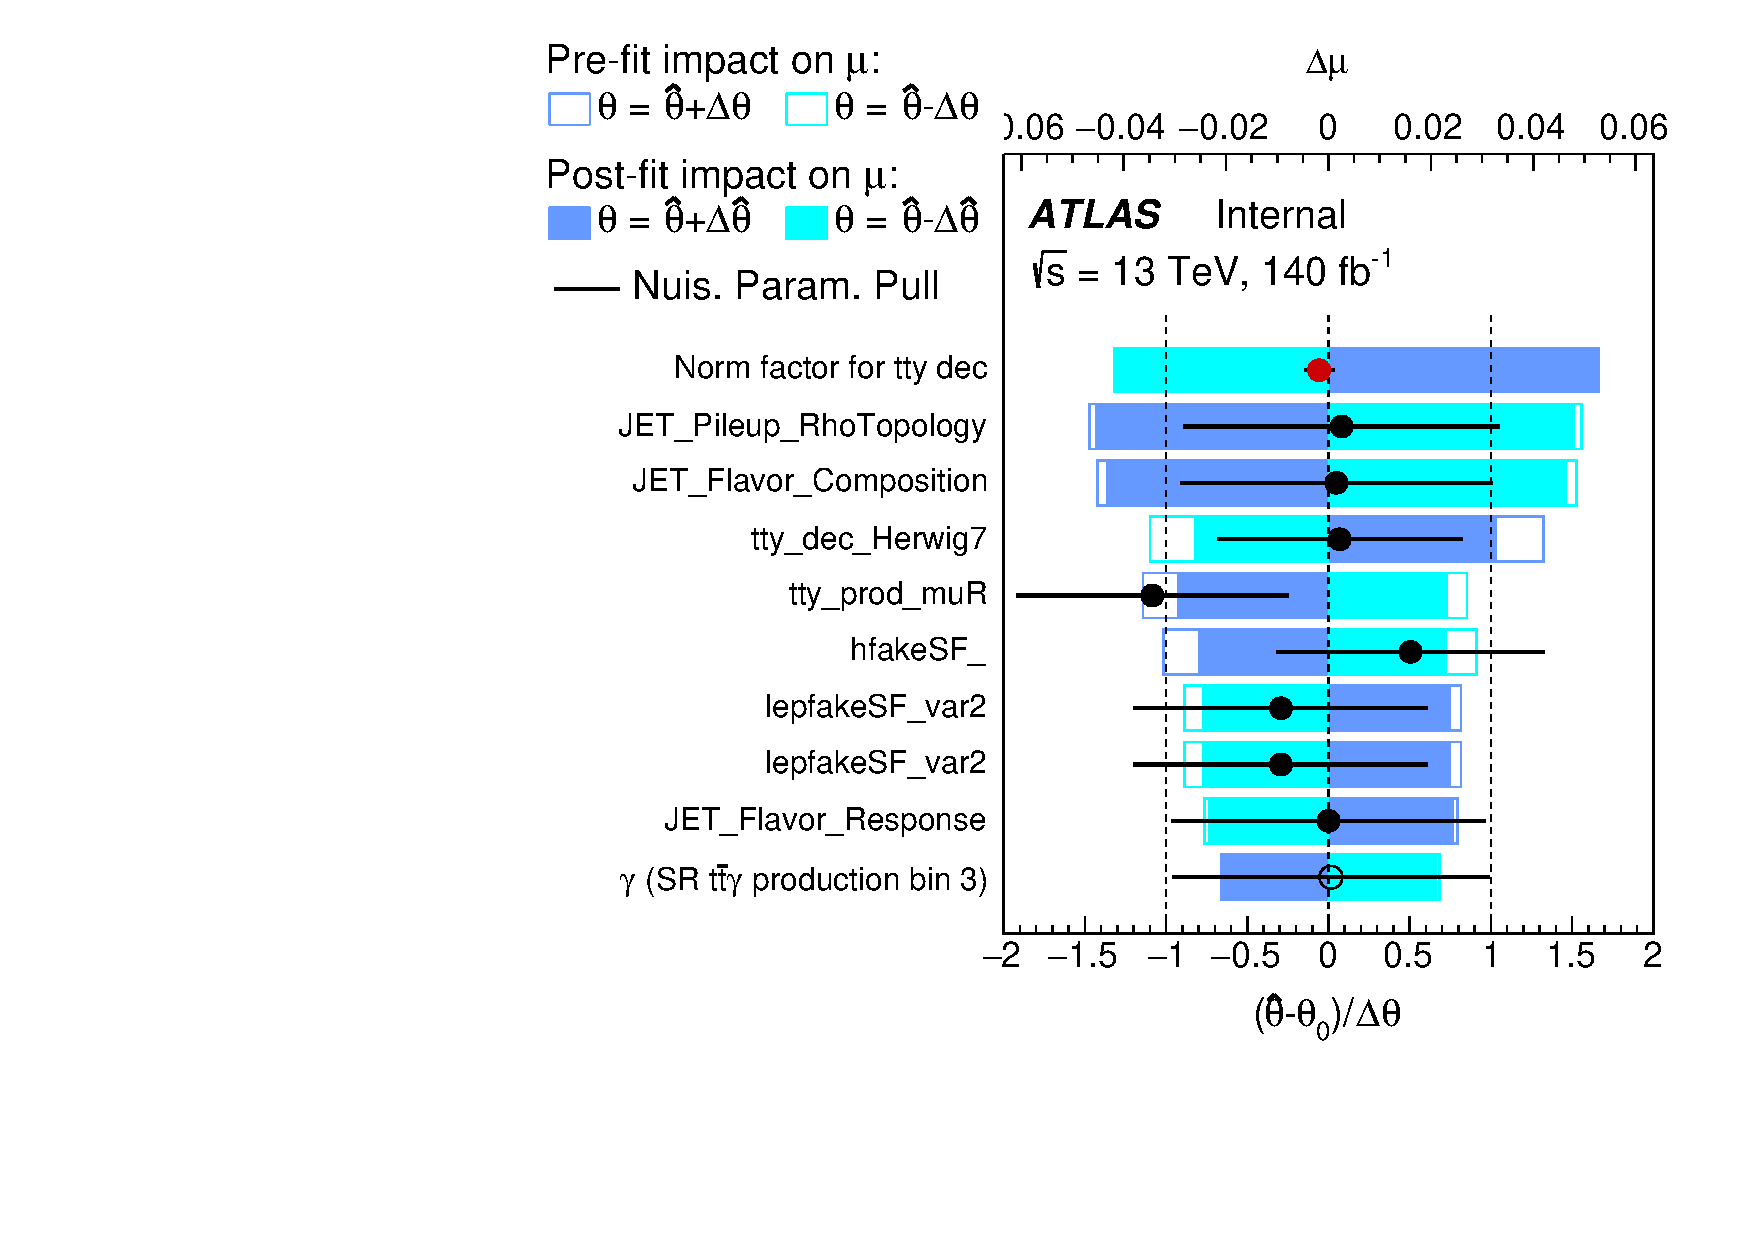
\includegraphics[width=0.33\textwidth]{figures/diff_xsec/ljet_tty_prod_mu_blinded/Ranking/tty1l_pt_all_syst/Ranking_tty_pt_Bin_004_mu.pdf}%
  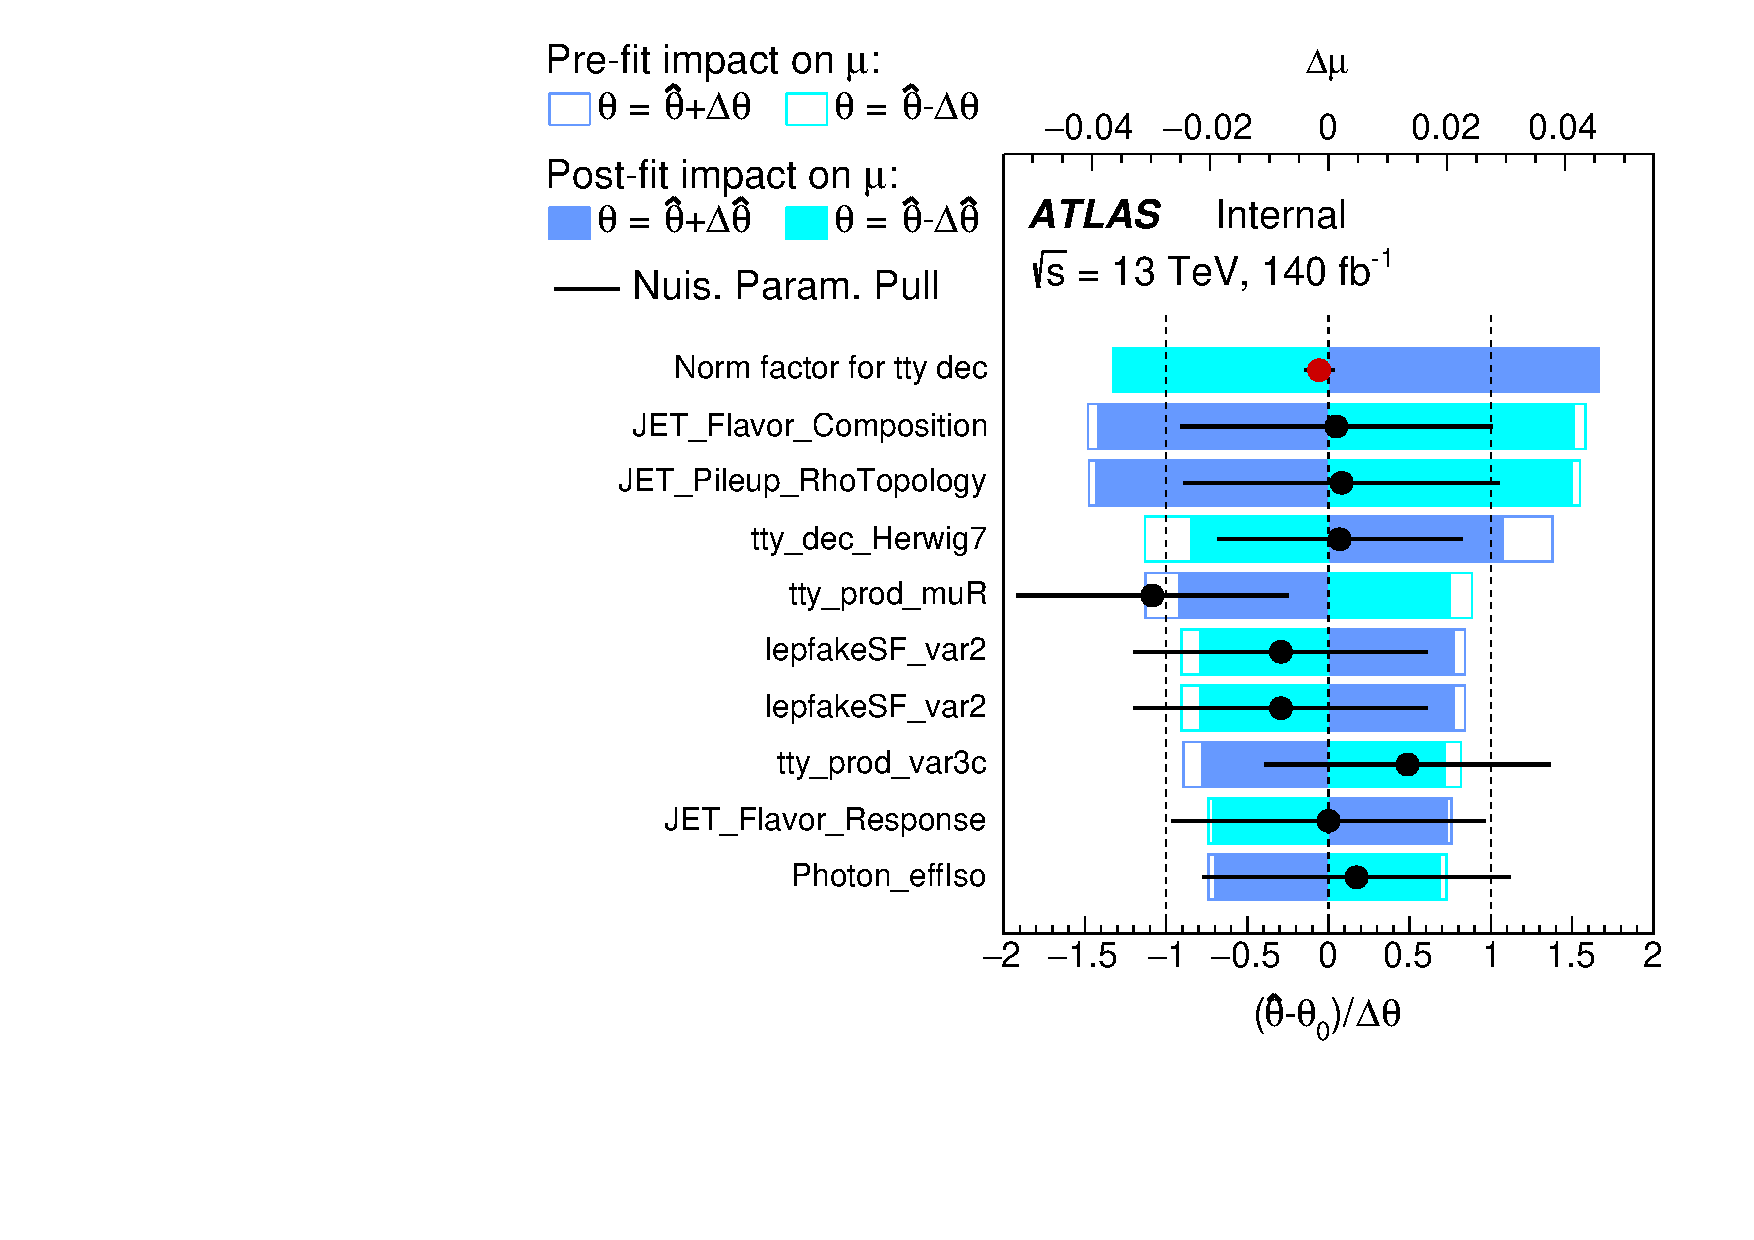
\includegraphics[width=0.33\textwidth]{figures/diff_xsec/ljet_tty_prod_mu_blinded/Ranking/tty1l_pt_all_syst/Ranking_tty_pt_Bin_005_mu.pdf}%
  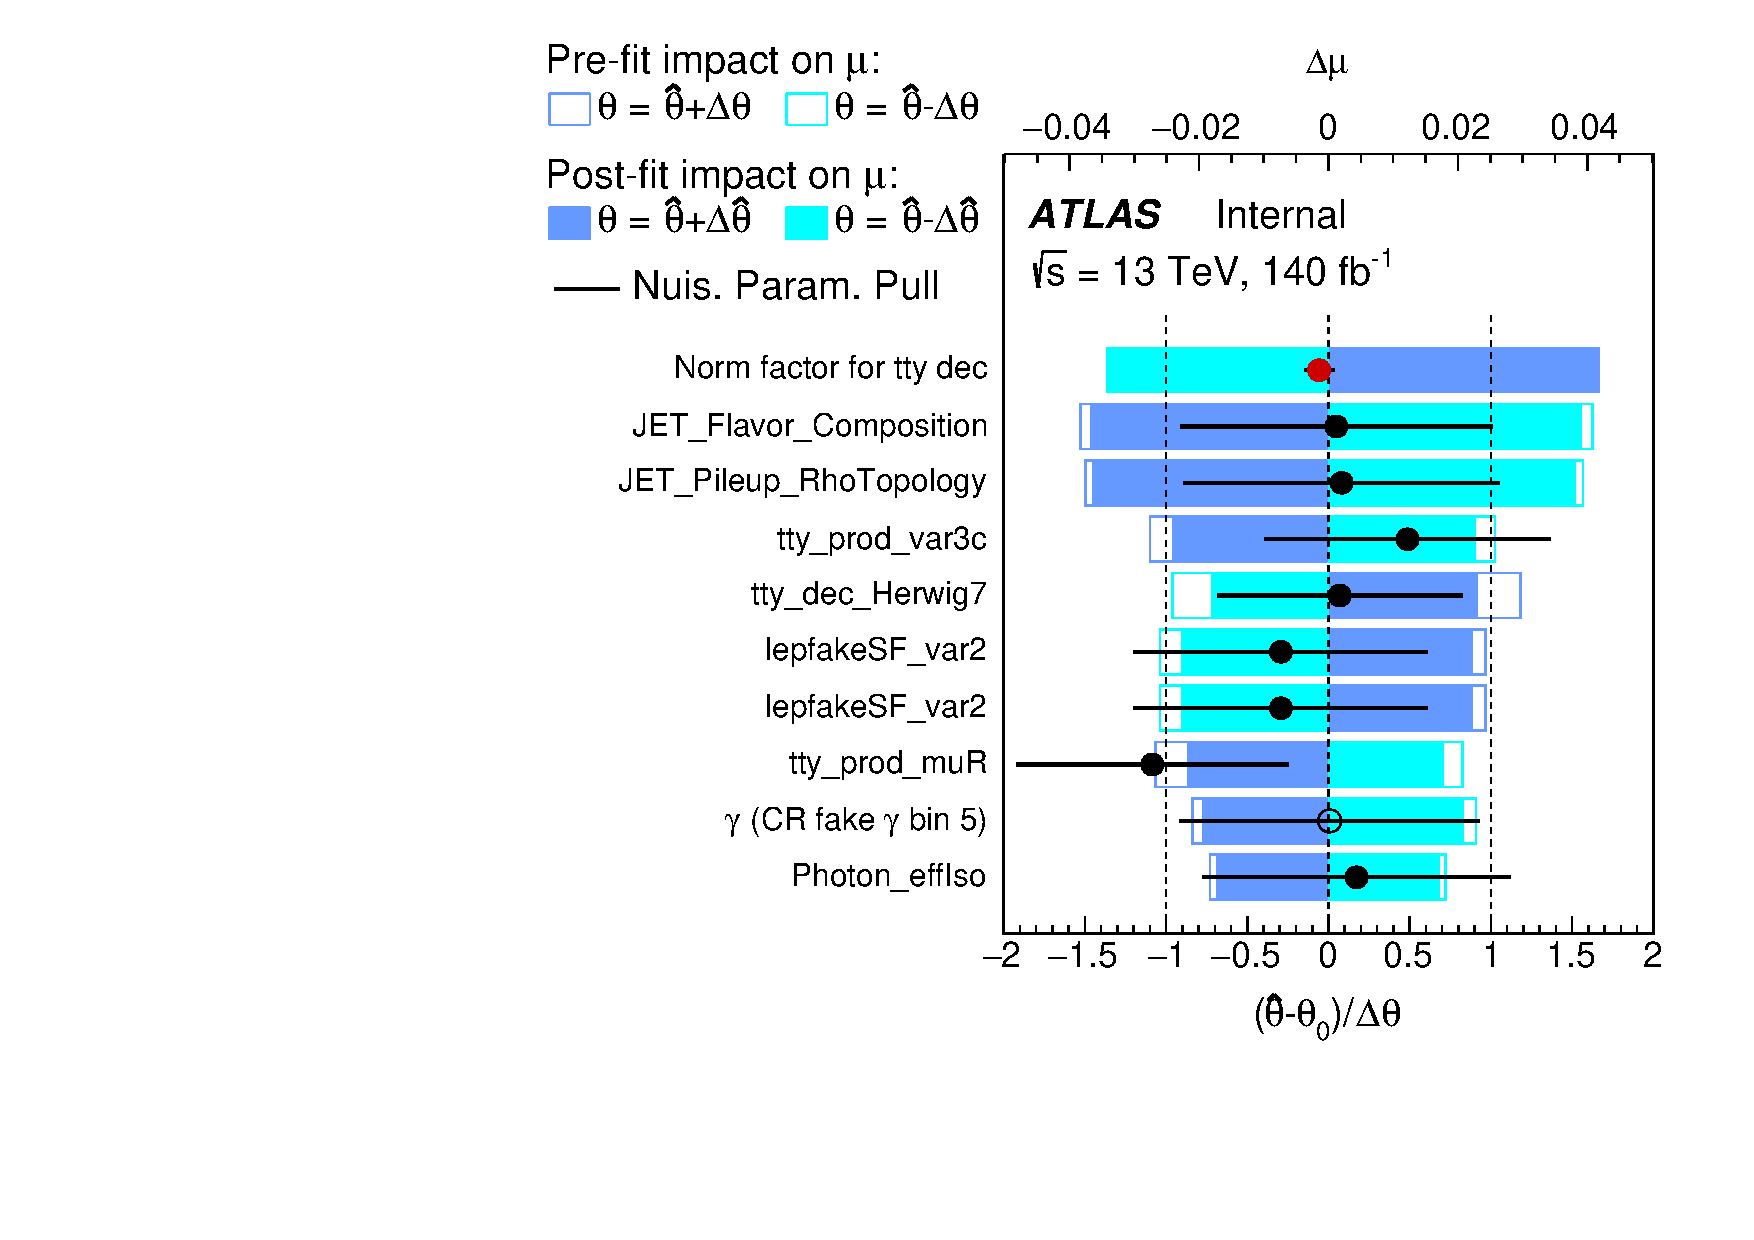
\includegraphics[width=0.33\textwidth]{figures/diff_xsec/ljet_tty_prod_mu_blinded/Ranking/tty1l_pt_all_syst/Ranking_tty_pt_Bin_006_mu.pdf}\\
  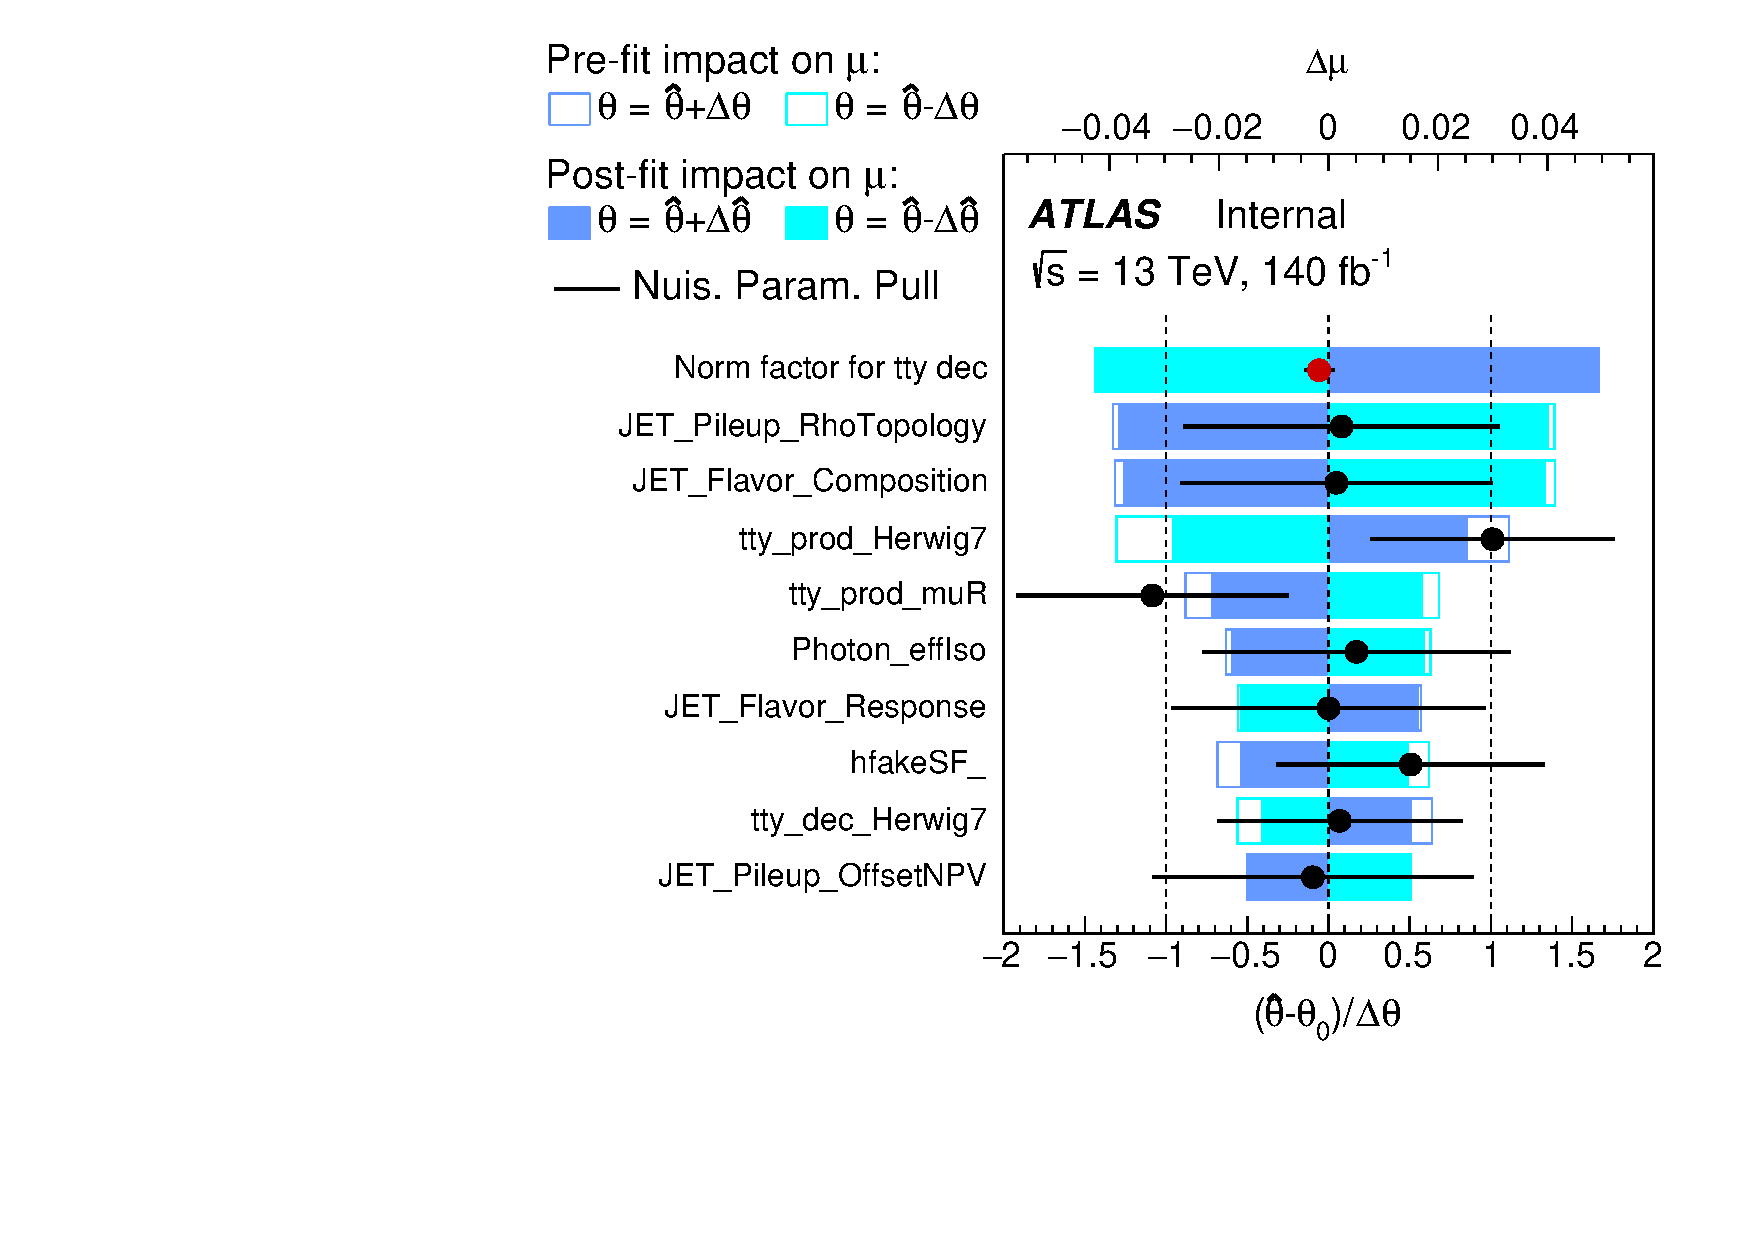
\includegraphics[width=0.33\textwidth]{figures/diff_xsec/ljet_tty_prod_mu_blinded/Ranking/tty1l_pt_all_syst/Ranking_tty_pt_Bin_007_mu.pdf}%
  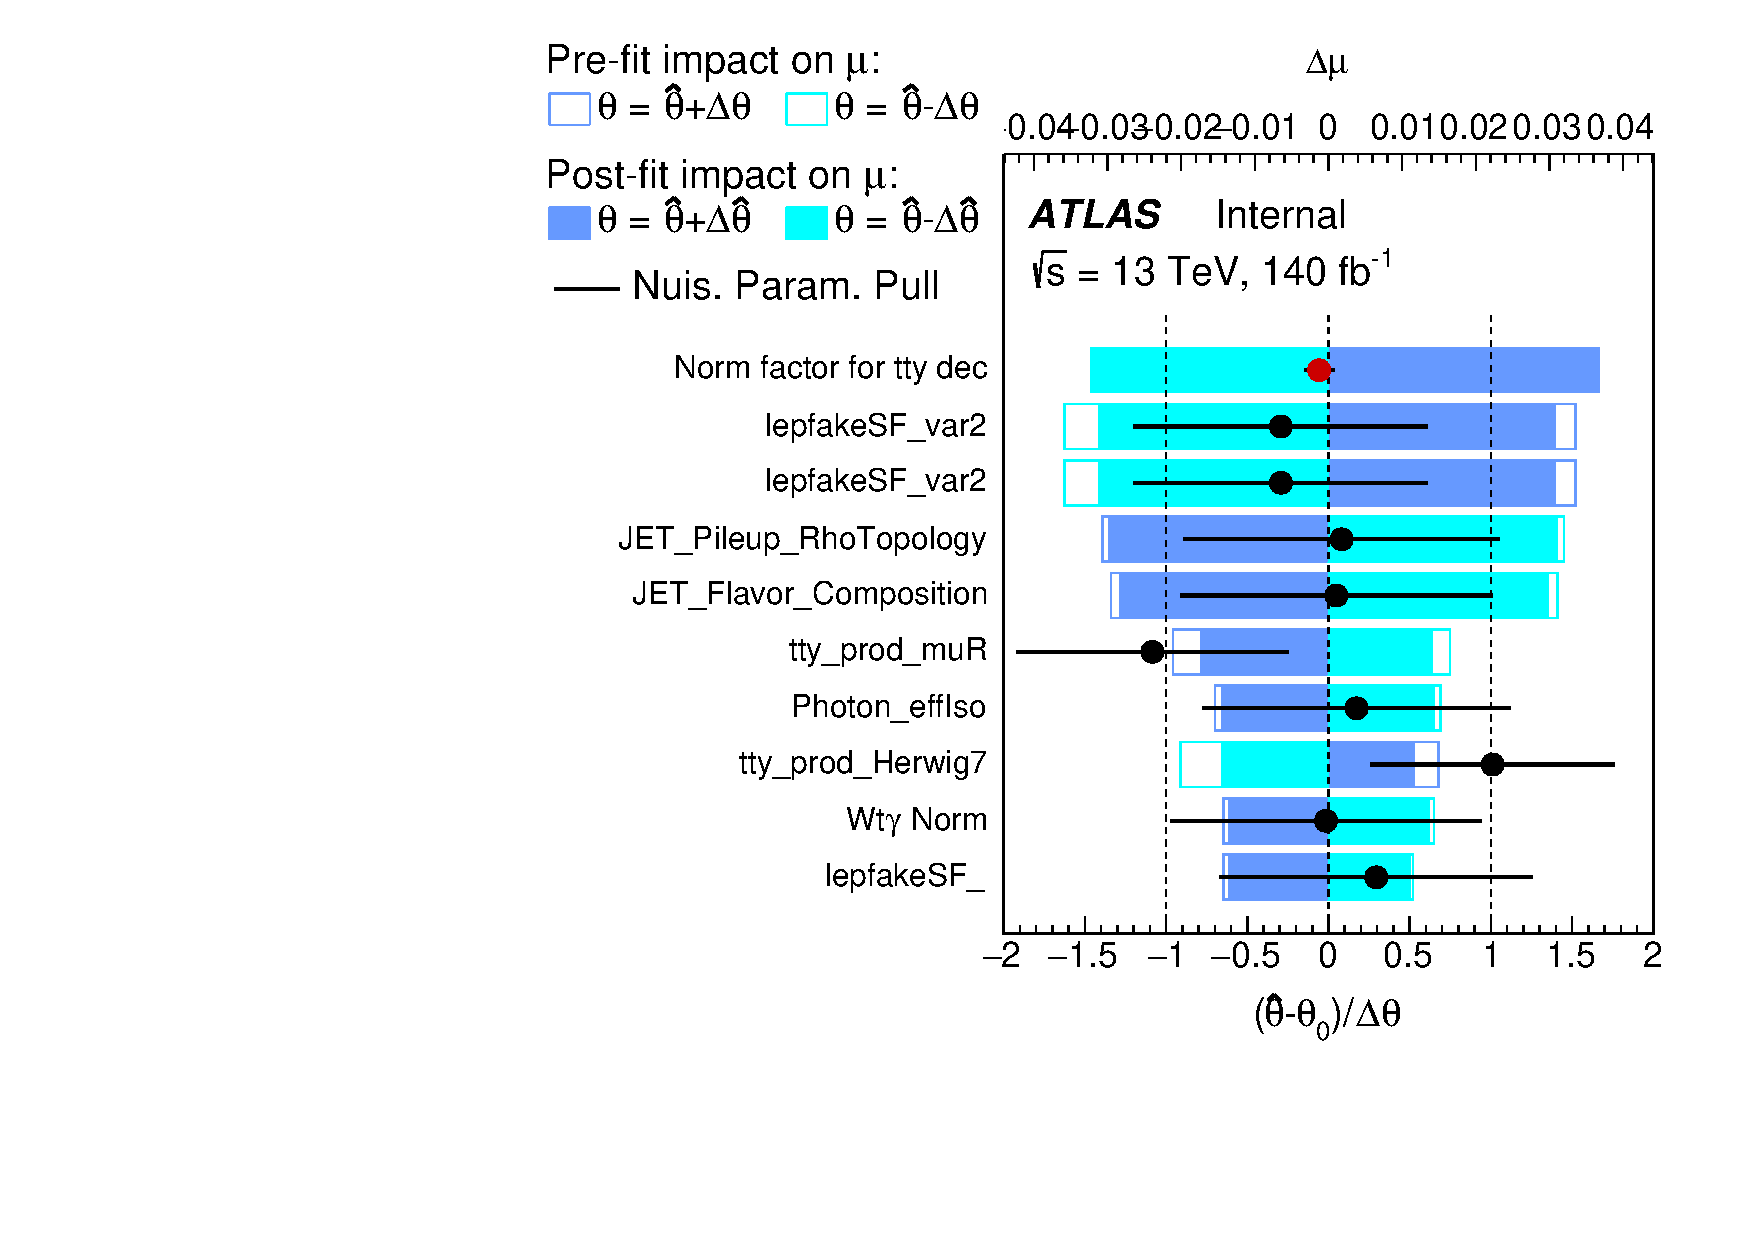
\includegraphics[width=0.33\textwidth]{figures/diff_xsec/ljet_tty_prod_mu_blinded/Ranking/tty1l_pt_all_syst/Ranking_tty_pt_Bin_008_mu.pdf}%
  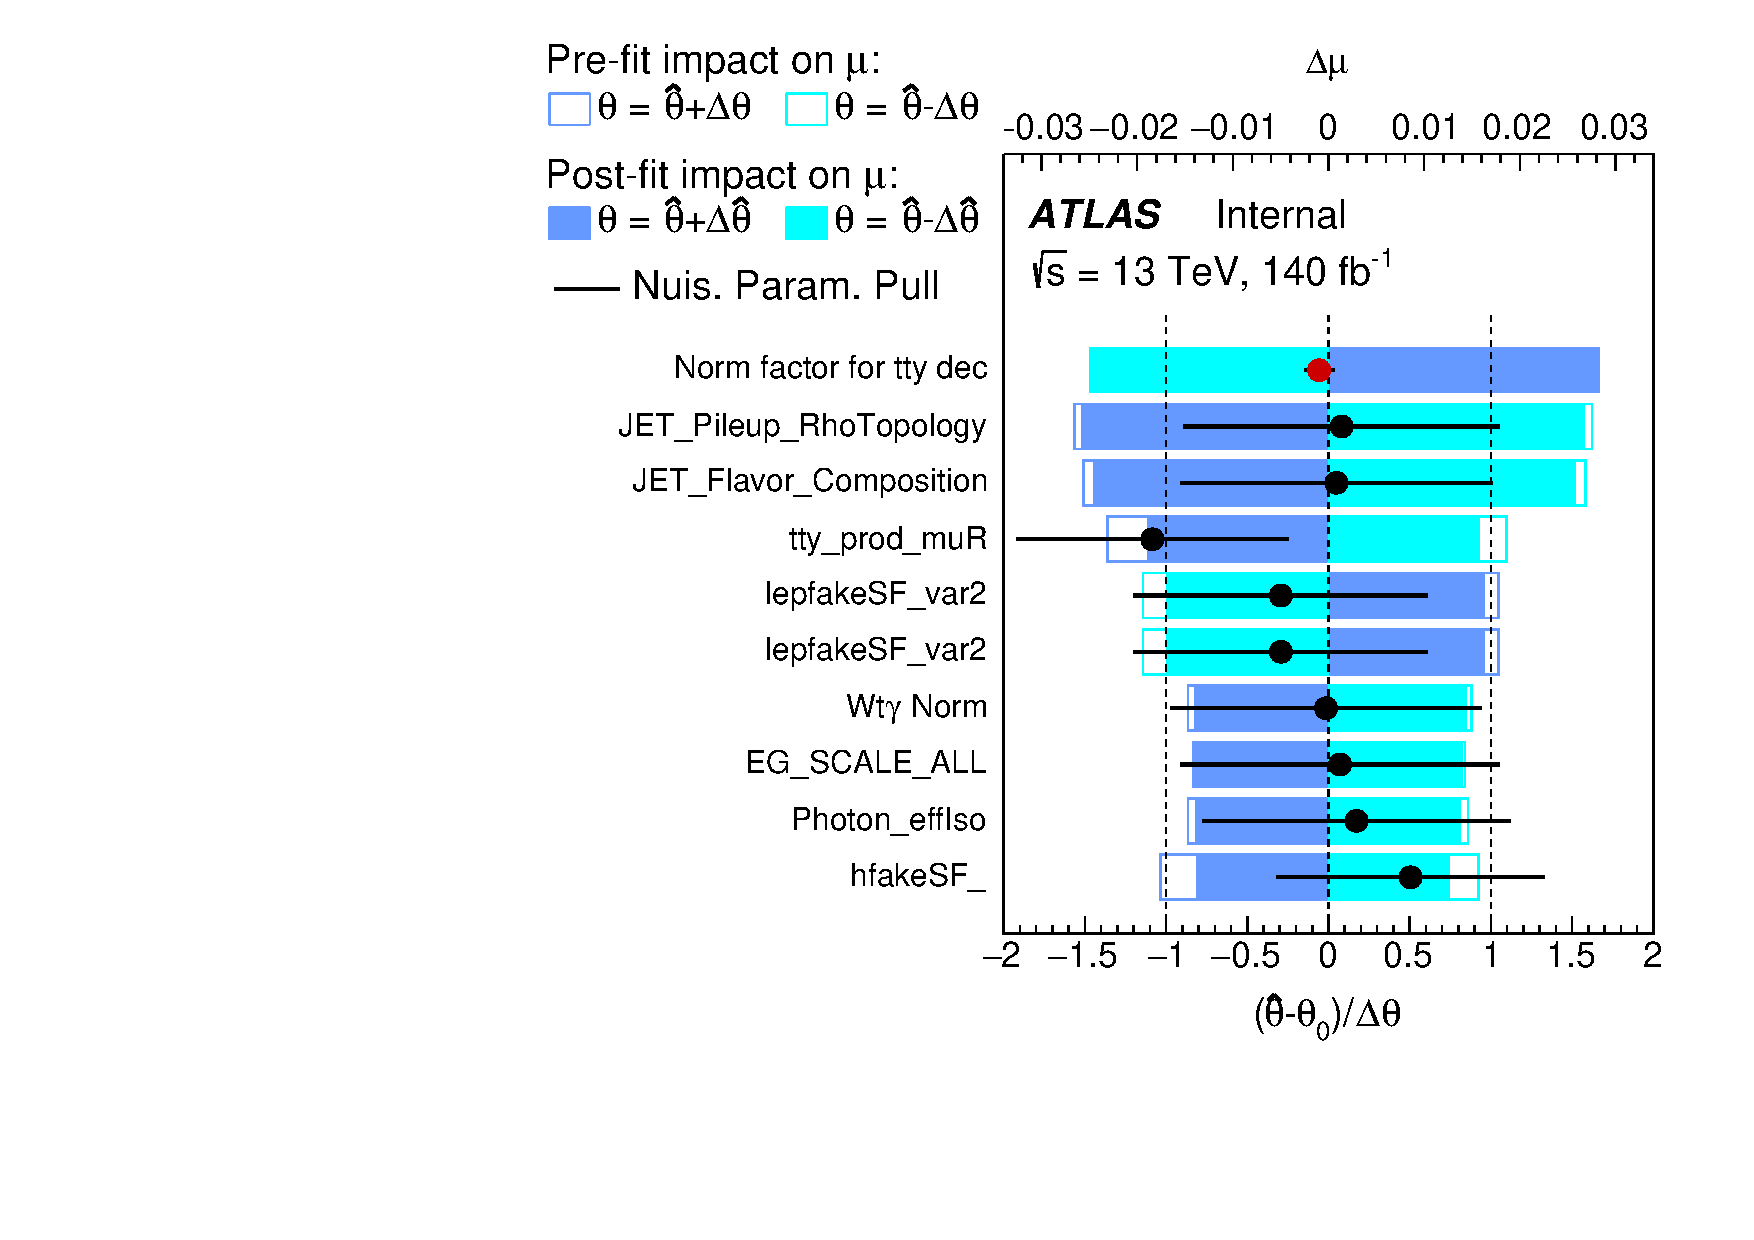
\includegraphics[width=0.33\textwidth]{figures/diff_xsec/ljet_tty_prod_mu_blinded/Ranking/tty1l_pt_all_syst/Ranking_tty_pt_Bin_009_mu.pdf}\\
  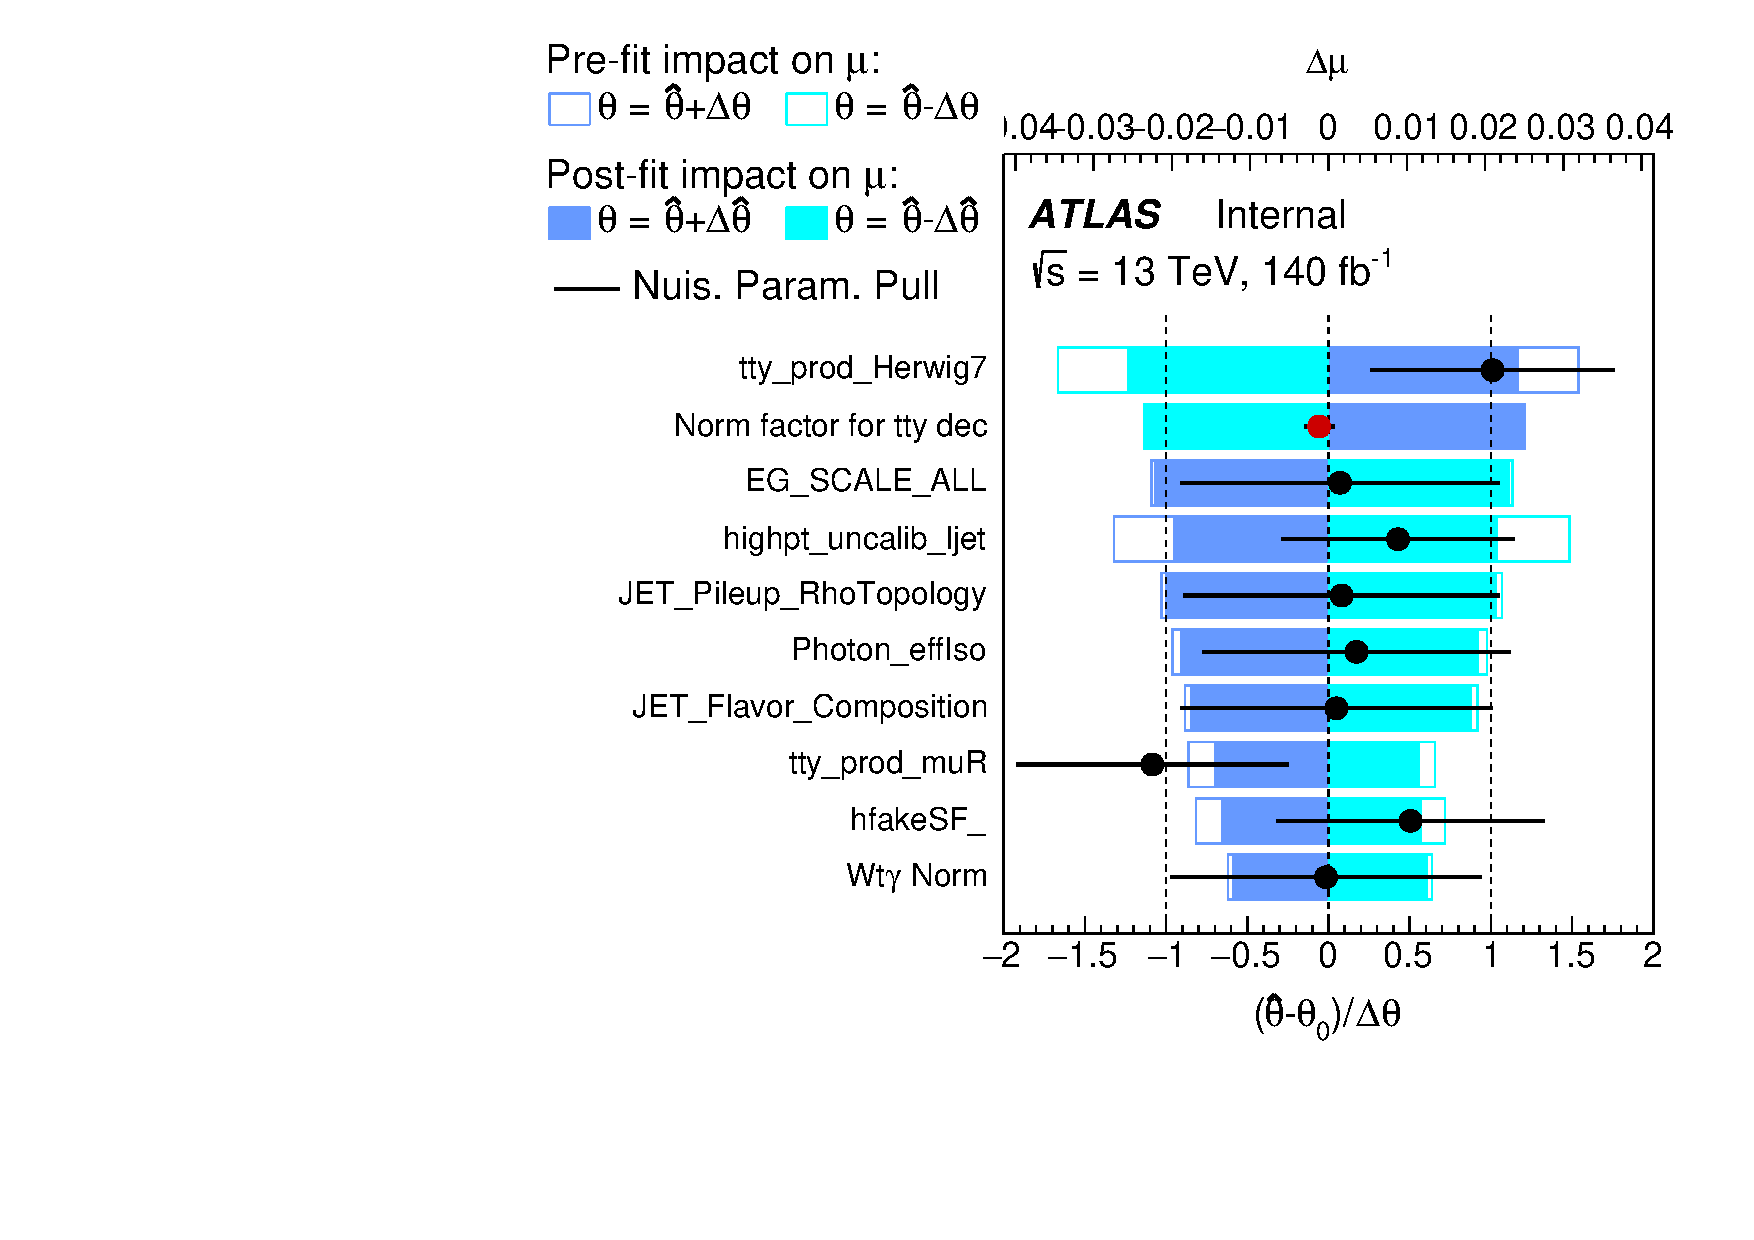
\includegraphics[width=0.33\textwidth]{figures/diff_xsec/ljet_tty_prod_mu_blinded/Ranking/tty1l_pt_all_syst/Ranking_tty_pt_Bin_010_mu.pdf}%
  \caption{Ranking plots showing the 10 NPs with the largest impact on the \tty production signal strength in each bin of the \ptgamma distribution in the single-lepton channel. Each subfigure, labeled (a), (b), (c), (d), ... (j), corresponds to a specific bin of the \ptgamma distribution, with bin 1 represented in subfigure (a), bin 2 represented in subfigure (b), and so on.}
  \label{fig:ranking_ljet_prod}
\end{figure}
\FloatBarrier


\begin{figure}[ht]
  \centering
  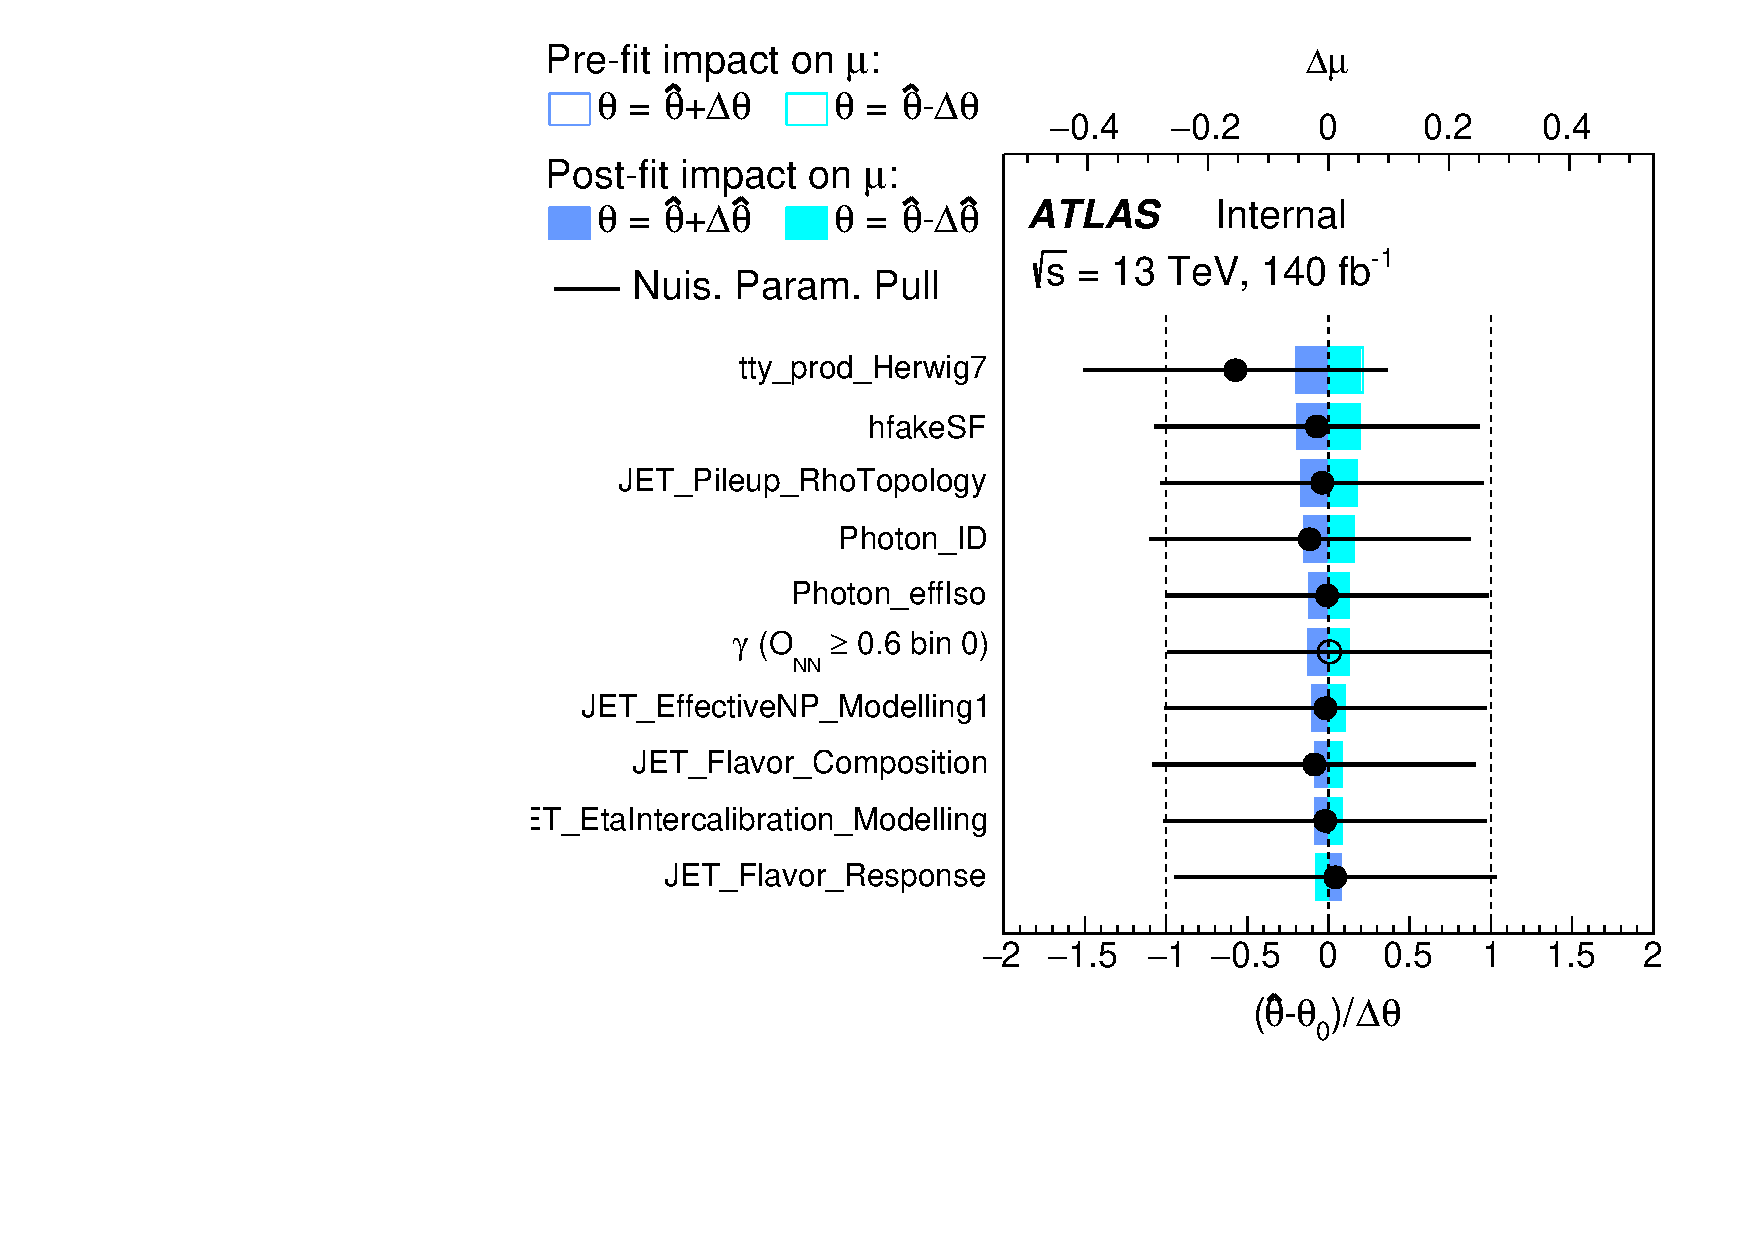
\includegraphics[width=0.33\textwidth]{figures/diff_xsec/dilep_tty_prod_mu_blinded/Ranking/tty2l_pt_all_syst/Ranking_tty_pt_Bin_001_mu.pdf}%
  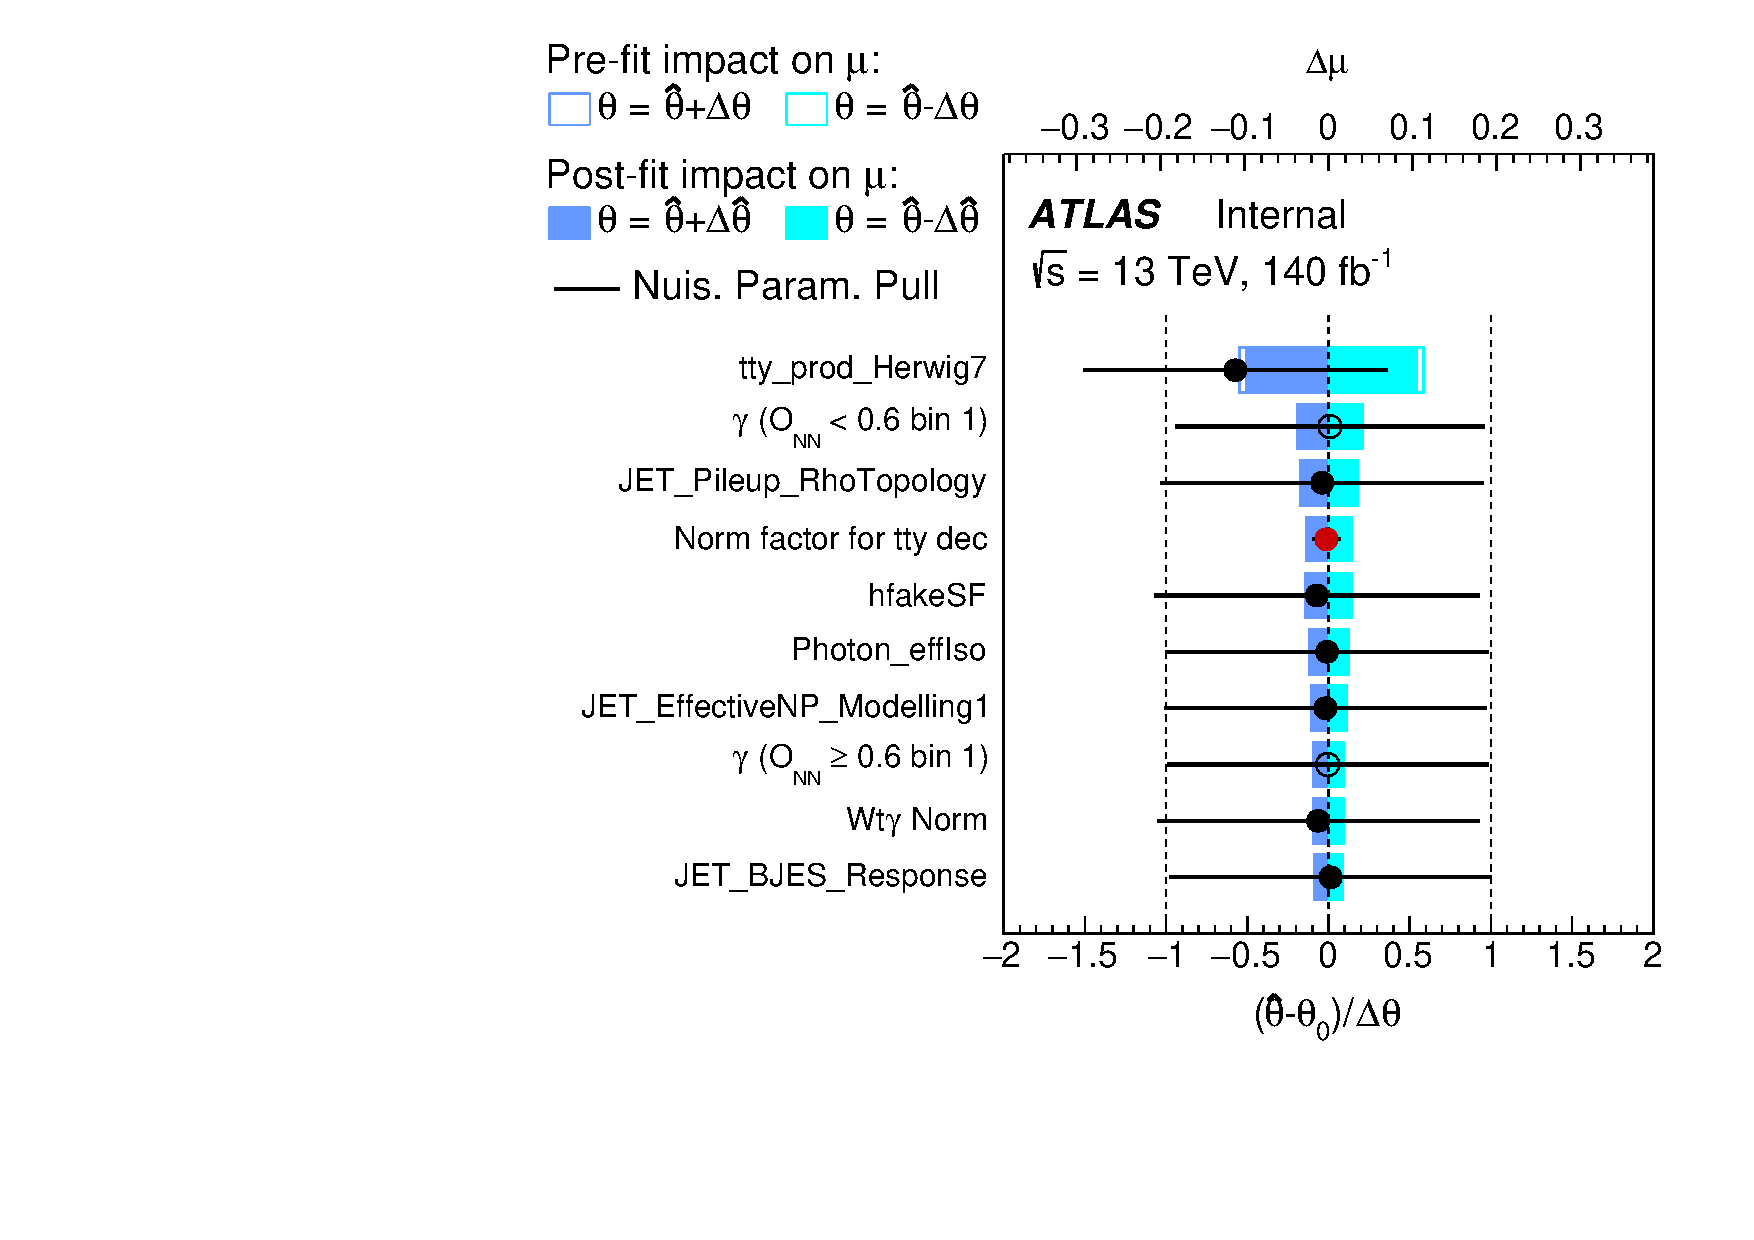
\includegraphics[width=0.33\textwidth]{figures/diff_xsec/dilep_tty_prod_mu_blinded/Ranking/tty2l_pt_all_syst/Ranking_tty_pt_Bin_002_mu.pdf}%
  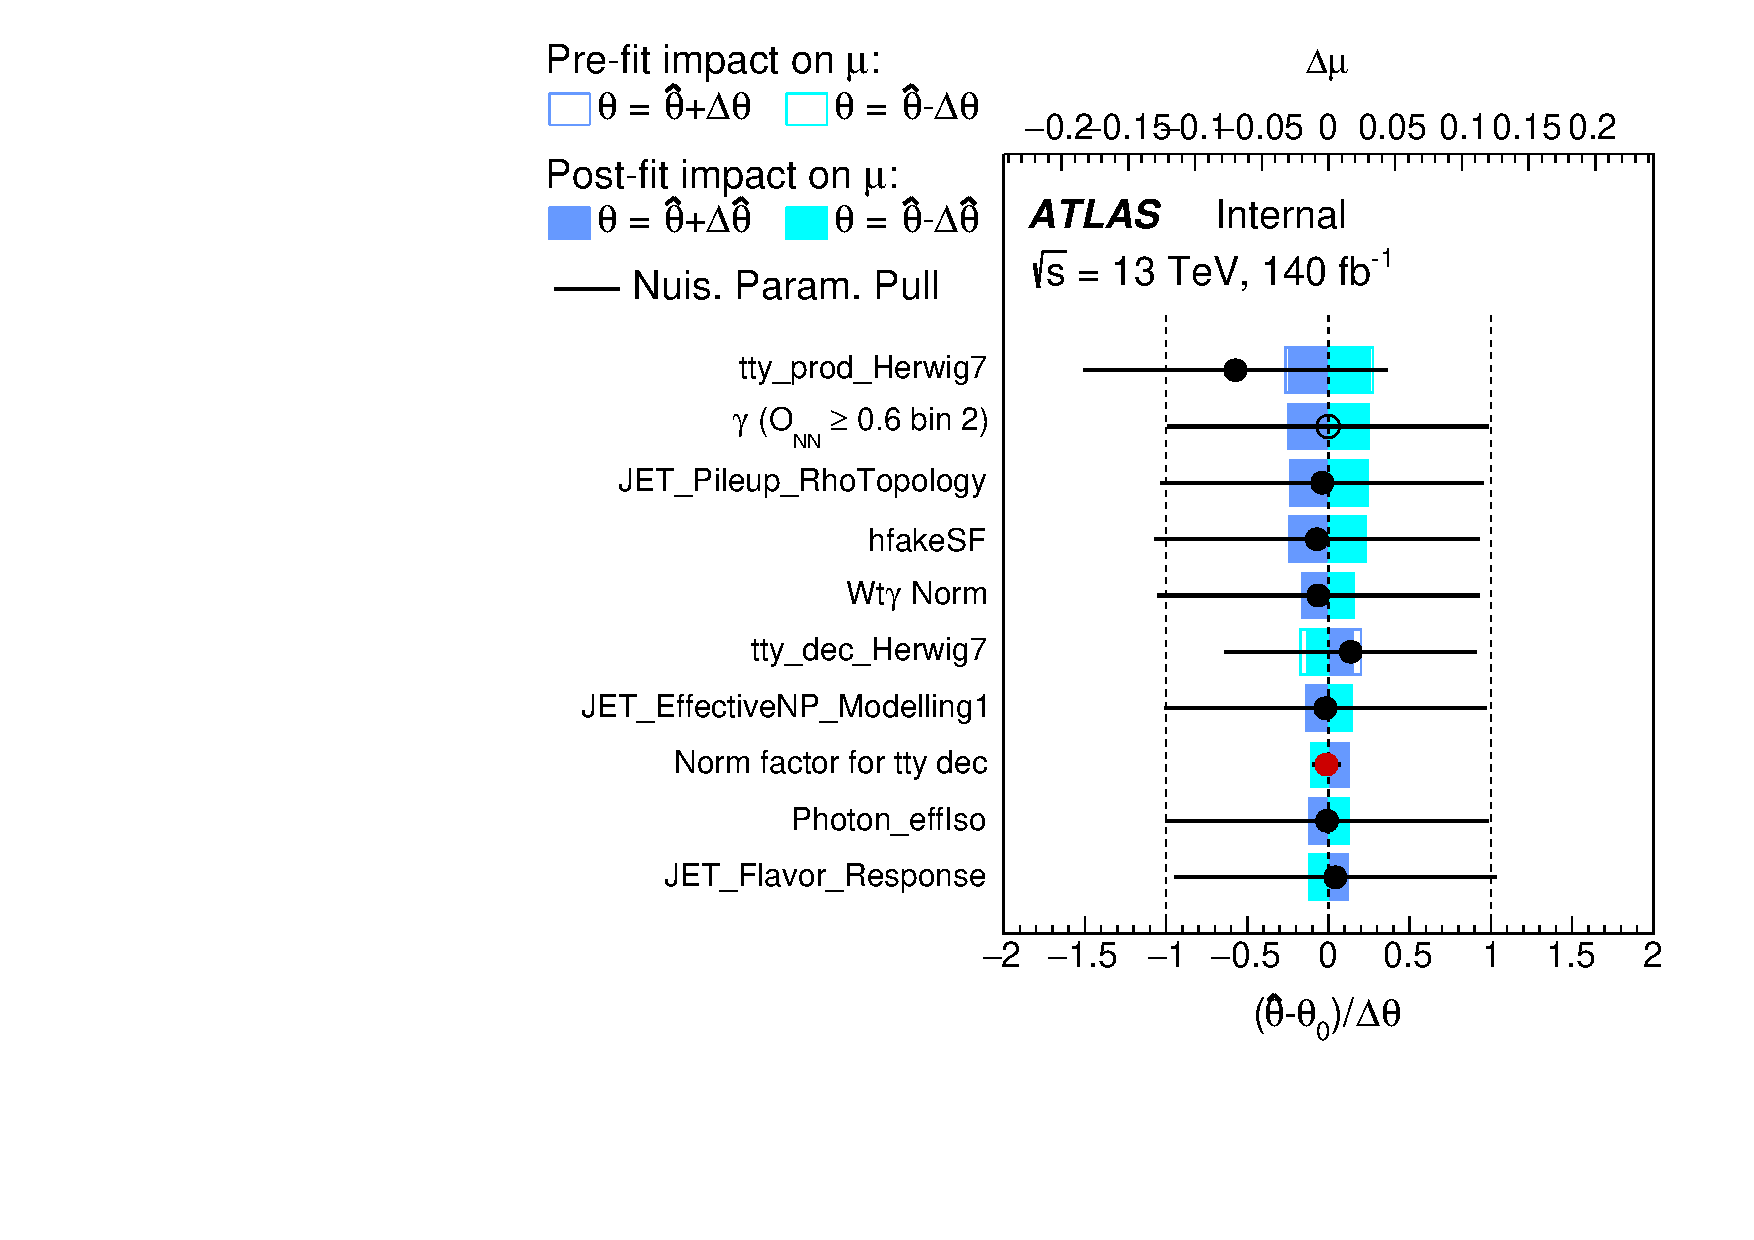
\includegraphics[width=0.33\textwidth]{figures/diff_xsec/dilep_tty_prod_mu_blinded/Ranking/tty2l_pt_all_syst/Ranking_tty_pt_Bin_003_mu.pdf}\\
  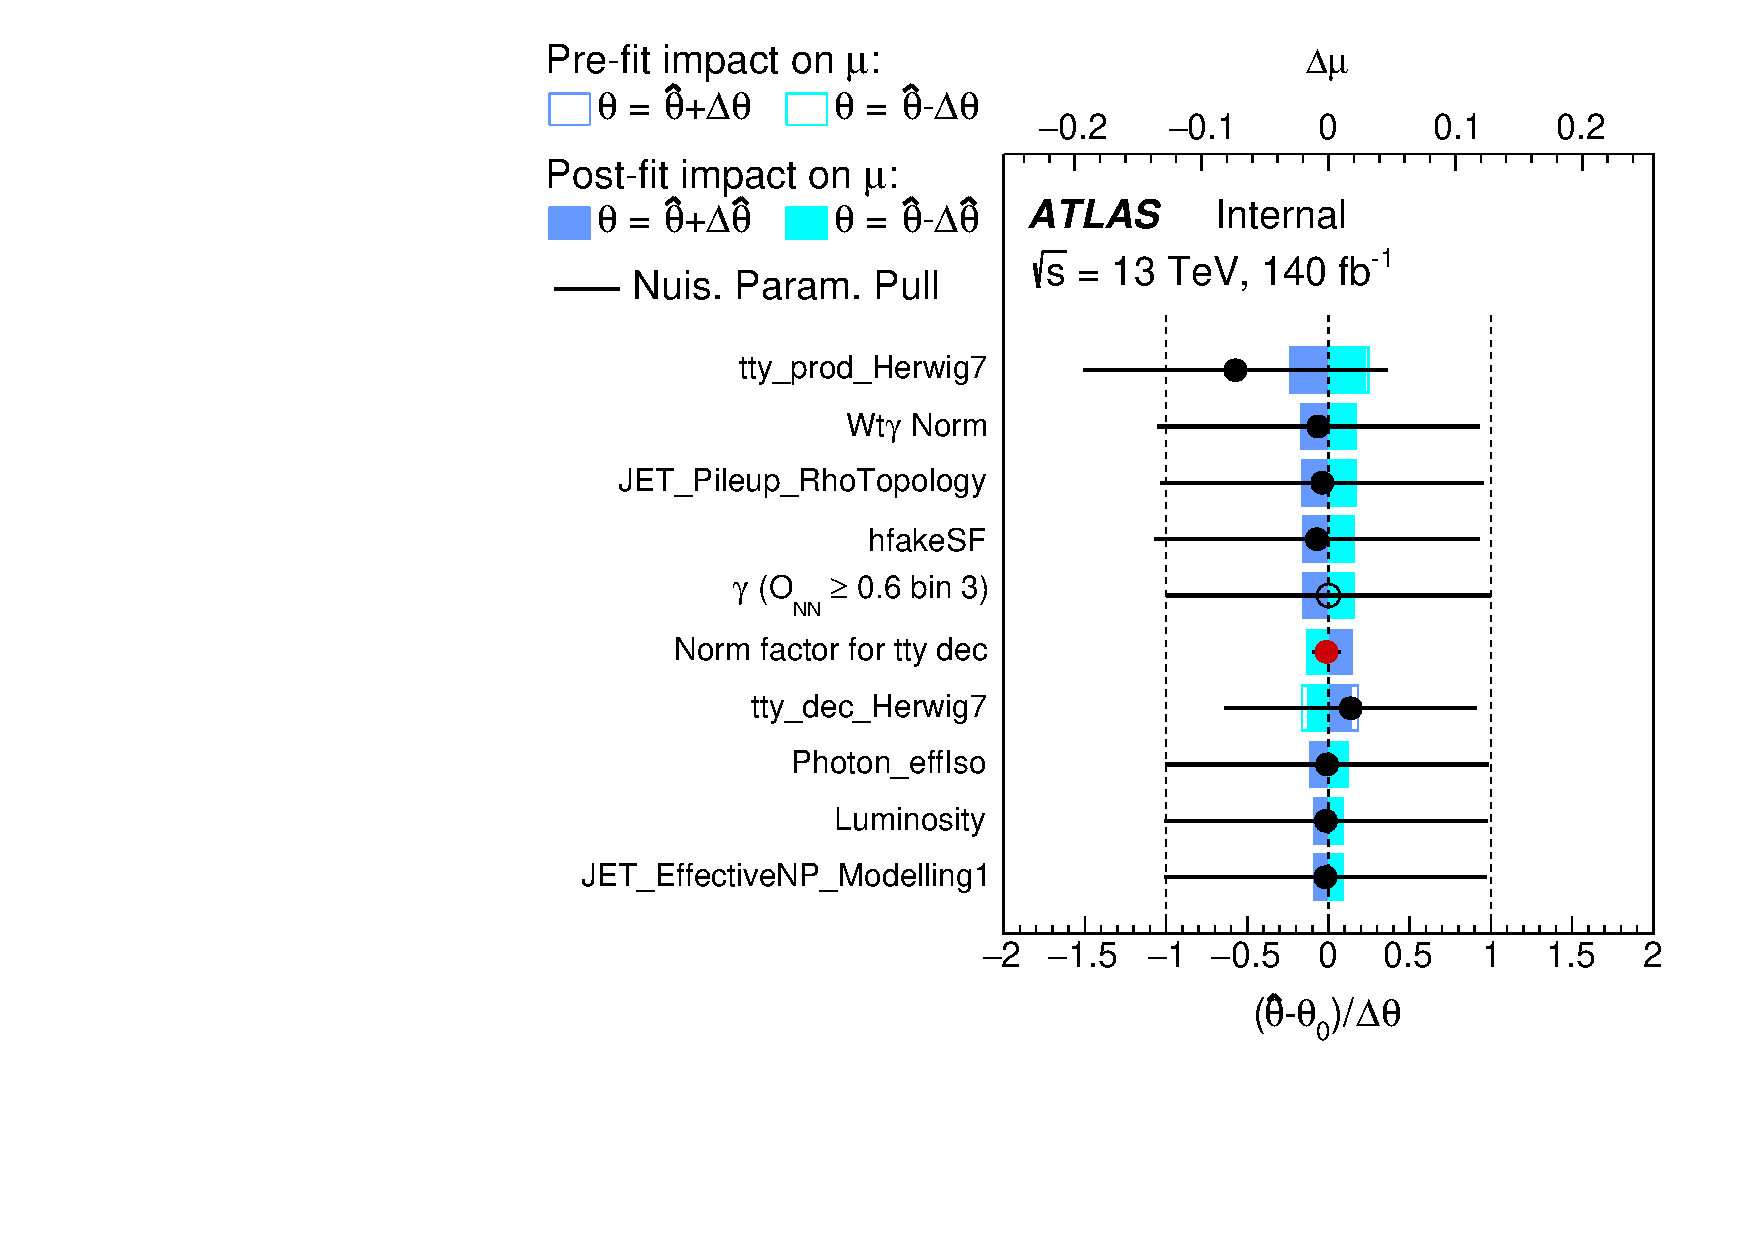
\includegraphics[width=0.33\textwidth]{figures/diff_xsec/dilep_tty_prod_mu_blinded/Ranking/tty2l_pt_all_syst/Ranking_tty_pt_Bin_004_mu.pdf}%
  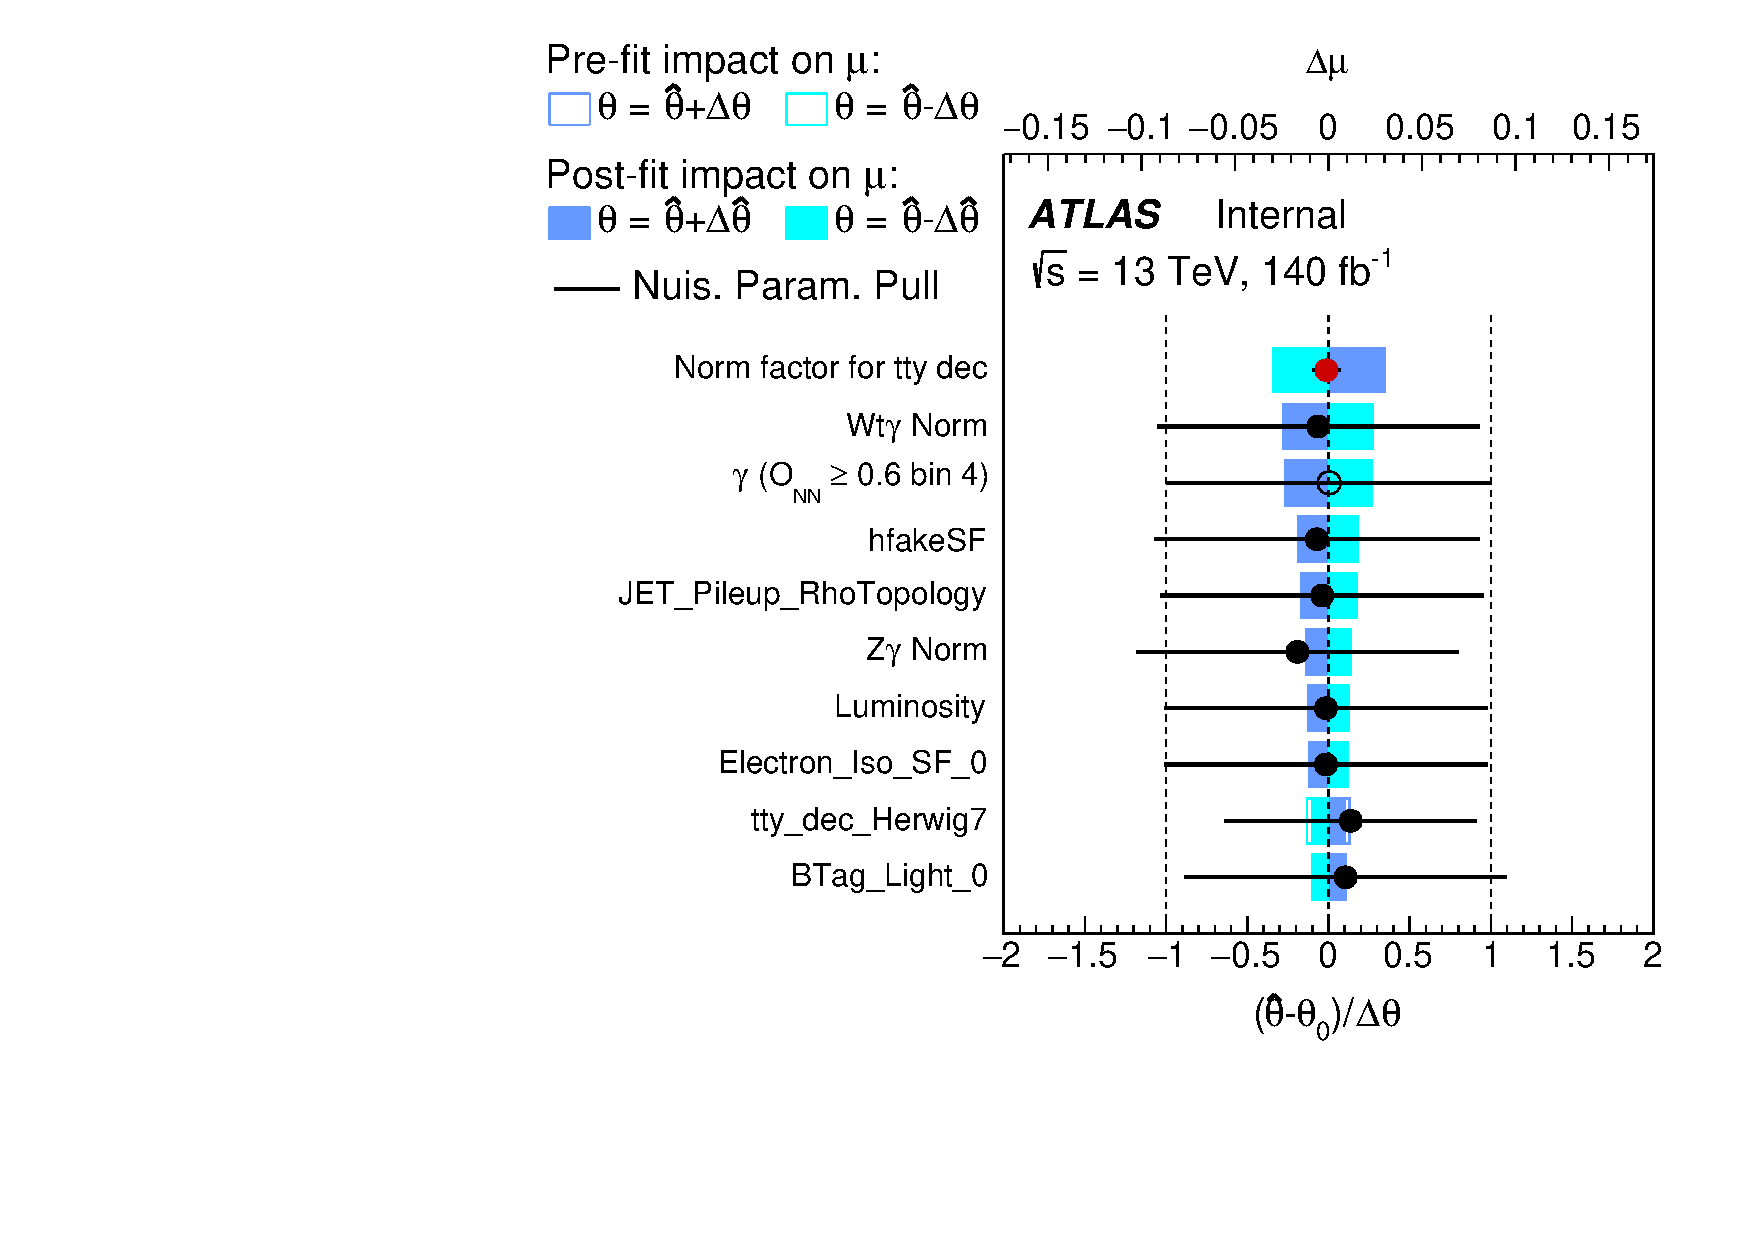
\includegraphics[width=0.33\textwidth]{figures/diff_xsec/dilep_tty_prod_mu_blinded/Ranking/tty2l_pt_all_syst/Ranking_tty_pt_Bin_005_mu.pdf}%
  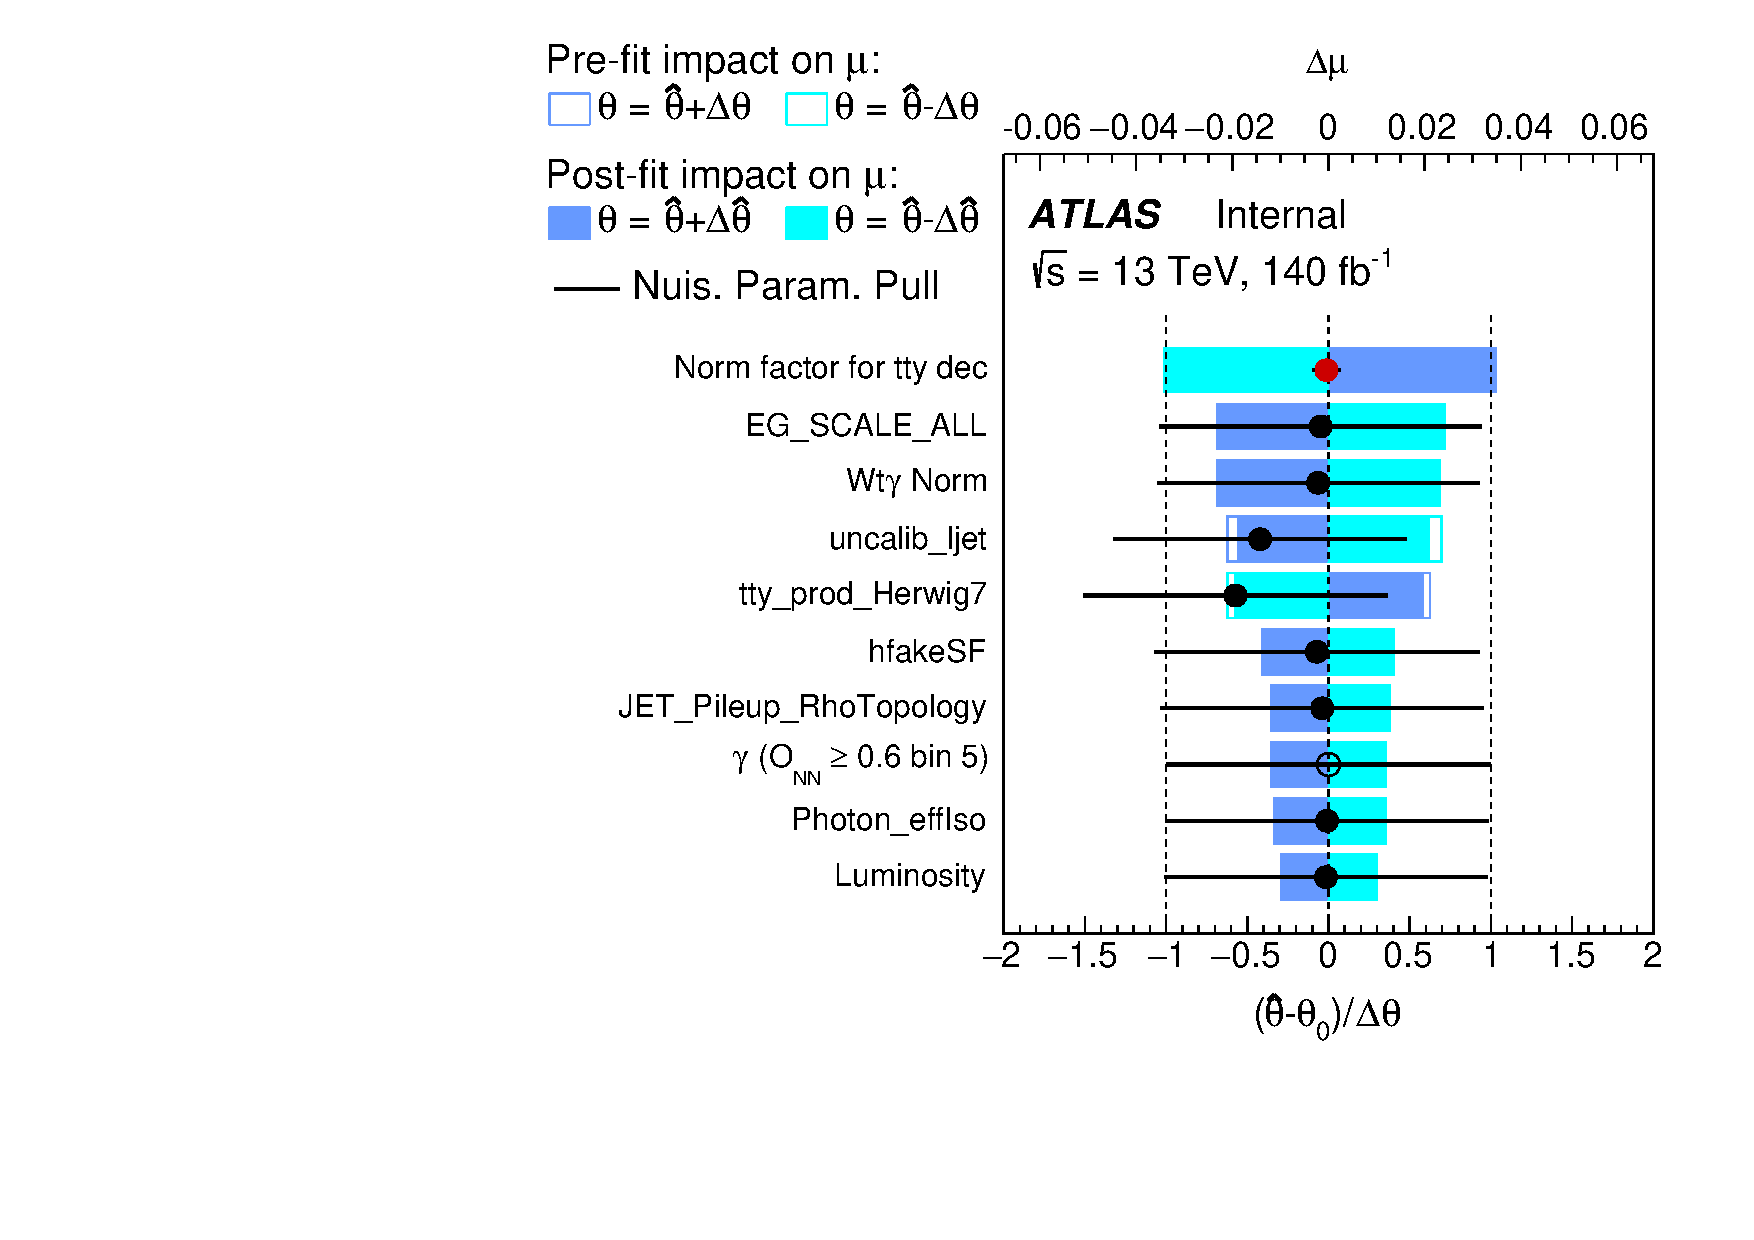
\includegraphics[width=0.33\textwidth]{figures/diff_xsec/dilep_tty_prod_mu_blinded/Ranking/tty2l_pt_all_syst/Ranking_tty_pt_Bin_006_mu.pdf}%
  \caption{Ranking plots showing the 10 NPs with the largest impact on the \tty production signal strength in each bin of the \ptgamma distribution in the dilepton channel. Each subfigure, labeled (a), (b), (c), (d), ... (j), corresponds to a specific bin of the \ptgamma distribution, with bin 1 represented in subfigure (a), bin 2 represented in subfigure (b), and so on.}
  \label{fig:ranking_dilep_prod}
\end{figure}
\FloatBarrier

\begin{figure}[ht]
  \centering
  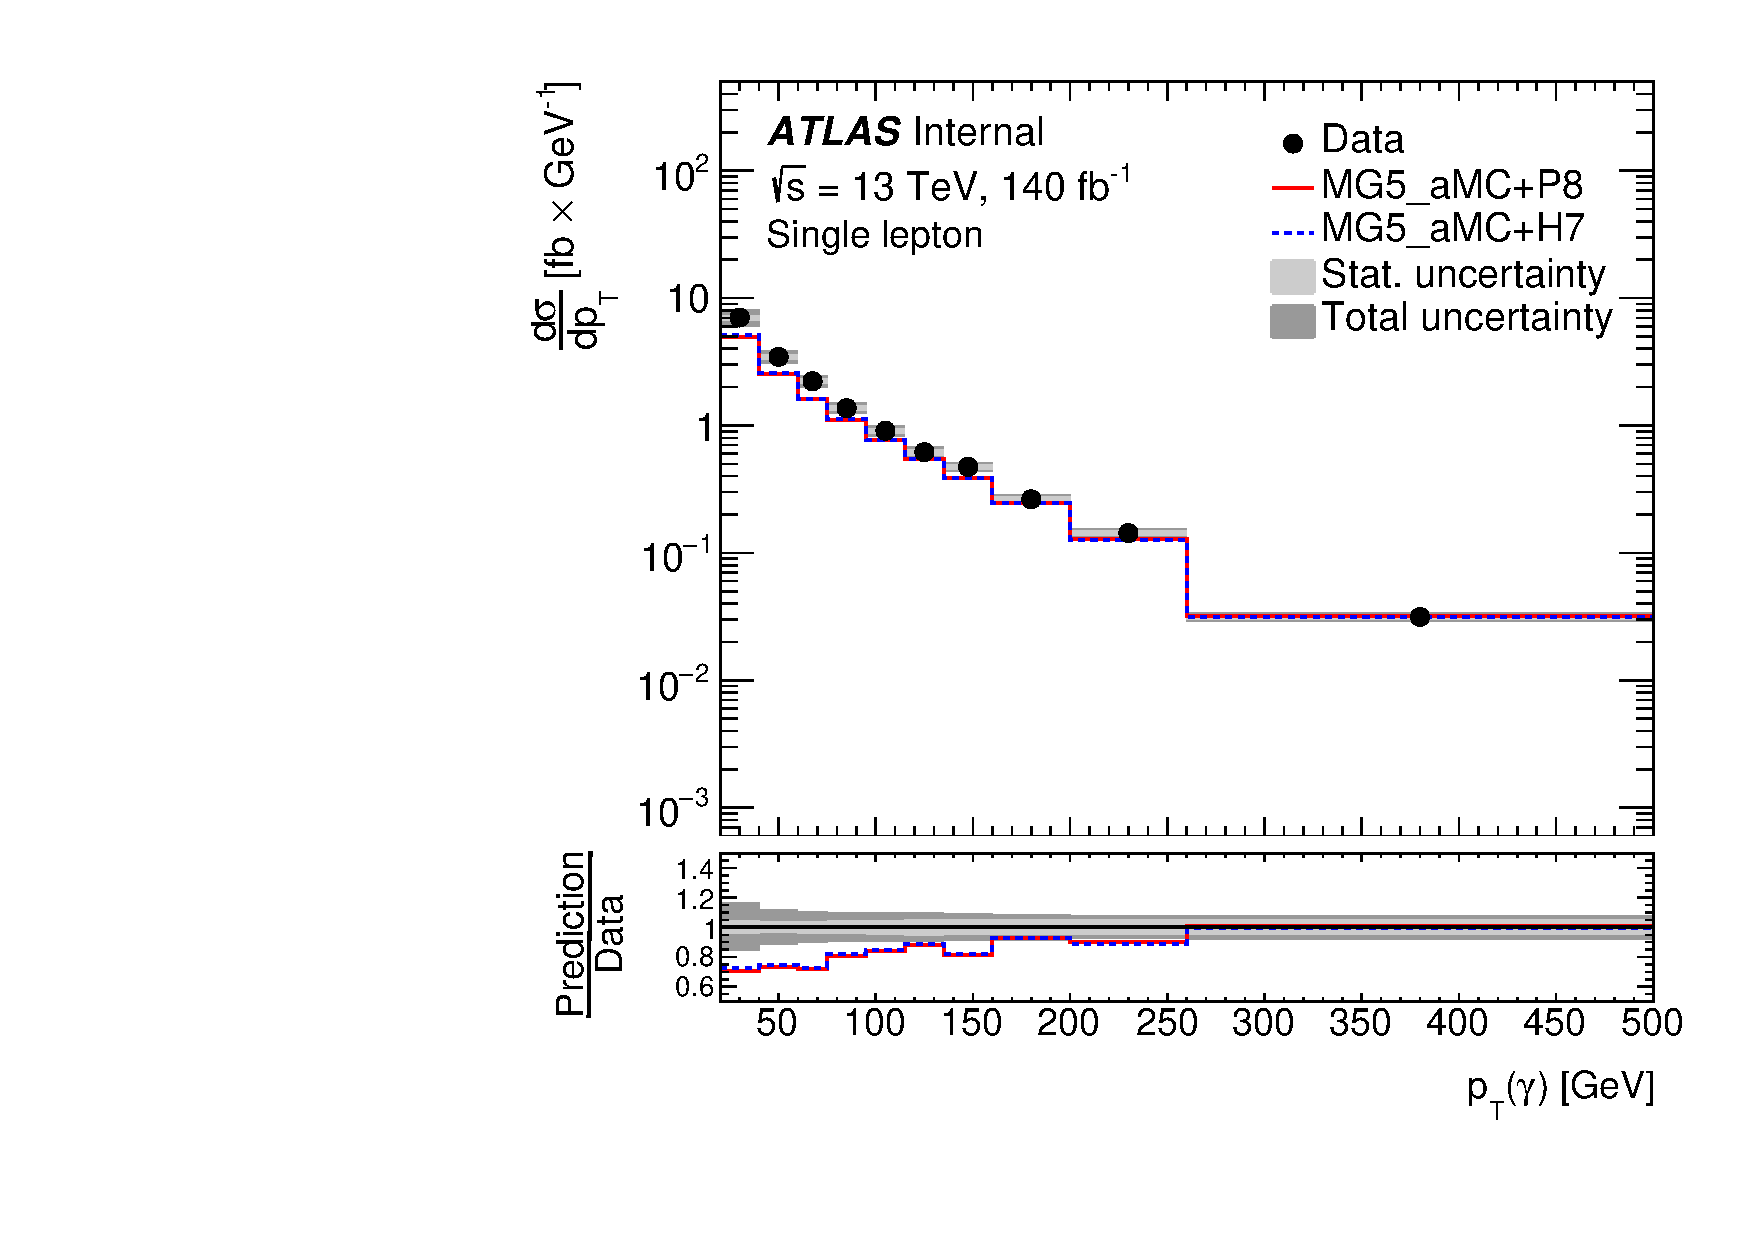
\includegraphics[width=0.33\textwidth]{figures/diff_xsec/absolute-unfolded-distributions/tty_prod_ljet/SL_tty_prod_pt_unfolded_absolute.pdf}%
  \includegraphics[width=0.33\textwidth]{figures/diff_xsec/absolute-unfolded-distributions/tty_prod_ljet/SL_tty_prod_eta_unfolded_absolute.pdf}%
  \includegraphics[width=0.33\textwidth]{figures/diff_xsec/absolute-unfolded-distributions/tty_prod_ljet/SL_tty_prod_drphl_unfolded_absolute.pdf}\\
  \includegraphics[width=0.33\textwidth]{figures/diff_xsec/absolute-unfolded-distributions/tty_prod_ljet/SL_tty_prod_drphb_unfolded_absolute.pdf}%
  \includegraphics[width=0.33\textwidth]{figures/diff_xsec/absolute-unfolded-distributions/tty_prod_ljet/SL_tty_prod_drlj_unfolded_absolute.pdf}%
  \includegraphics[width=0.33\textwidth]{figures/diff_xsec/absolute-unfolded-distributions/tty_prod_ljet/SL_tty_prod_ptj1_unfolded_absolute.pdf}%
  \caption{Absolute differential cross-sections of \tty production in single-lepton fiducial phase space as a function of several observables. Data are compared with \madgraph simulation interfaced with \pythia and \herwig. The last bin includes overflow events.}
  \label{fig:pt_unfolded_ljet_dist_realdata}
\end{figure}
\FloatBarrier



\begin{figure}[ht]
  \centering
  \includegraphics[width=0.33\textwidth]{figures/diff_xsec/absolute-unfolded-distributions/tty_prod_dilep/DL_tty_prod_pt_unfolded_absolute.pdf}%
  \includegraphics[width=0.33\textwidth]{figures/diff_xsec/absolute-unfolded-distributions/tty_prod_dilep/DL_tty_prod_eta_unfolded_absolute.pdf}%
  \includegraphics[width=0.33\textwidth]{figures/diff_xsec/absolute-unfolded-distributions/tty_prod_dilep/DL_tty_prod_drphl_unfolded_absolute.pdf}\\
  \includegraphics[width=0.33\textwidth]{figures/diff_xsec/absolute-unfolded-distributions/tty_prod_dilep/DL_tty_prod_drphl1_unfolded_absolute.pdf}%
  \includegraphics[width=0.33\textwidth]{figures/diff_xsec/absolute-unfolded-distributions/tty_prod_dilep/DL_tty_prod_drphl2_unfolded_absolute.pdf}%
  \includegraphics[width=0.33\textwidth]{figures/diff_xsec/absolute-unfolded-distributions/tty_prod_dilep/DL_tty_prod_dEtall_unfolded_absolute.pdf}%
  \caption{Absolute differential cross-sections of \tty production in dilepton fiducial phase space as a function of several observables. Data are compared with \madgraph simulation interfaced with \pythia and \herwig. The last bin includes overflow events.}
  \label{fig:pt_unfolded_dilep_dist_realdata_1}
\end{figure}

\begin{figure}[ht]
  \centering
  \includegraphics[width=0.33\textwidth]{figures/diff_xsec/absolute-unfolded-distributions/tty_prod_dilep/DL_tty_prod_dPhill_unfolded_absolute.pdf}%
  \includegraphics[width=0.33\textwidth]{figures/diff_xsec/absolute-unfolded-distributions/tty_prod_dilep/DL_tty_prod_ptll_unfolded_absolute.pdf}%
  \includegraphics[width=0.33\textwidth]{figures/diff_xsec/absolute-unfolded-distributions/tty_prod_dilep/DL_tty_prod_drphb_unfolded_absolute.pdf}\\
  \includegraphics[width=0.33\textwidth]{figures/diff_xsec/absolute-unfolded-distributions/tty_prod_dilep/DL_tty_prod_drlj_unfolded_absolute.pdf}%
  \includegraphics[width=0.33\textwidth]{figures/diff_xsec/absolute-unfolded-distributions/tty_prod_dilep/DL_tty_prod_ptj1_unfolded_absolute.pdf}%
  \caption{Absolute differential cross-sections of \tty production in dilepton fiducial phase space as a function of several observables. Data are compared with \madgraph simulation interfaced with \pythia and \herwig. The last bin includes overflow events.}
  \label{fig:pt_unfolded_dilep_dist_realdata_2}
\end{figure}
\FloatBarrier

\begin{figure}[ht]
  \centering
  \includegraphics[width=0.33\textwidth]{figures/diff_xsec/normalized-unfolded-distributions/tty_prod_ljet/SL_tty_prod_pt_unfolded_normalized.pdf}%
  \includegraphics[width=0.33\textwidth]{figures/diff_xsec/normalized-unfolded-distributions/tty_prod_ljet/SL_tty_prod_eta_unfolded_normalized.pdf}%
  \includegraphics[width=0.33\textwidth]{figures/diff_xsec/normalized-unfolded-distributions/tty_prod_ljet/SL_tty_prod_drphb_unfolded_normalized.pdf}\\
  \includegraphics[width=0.33\textwidth]{figures/diff_xsec/normalized-unfolded-distributions/tty_prod_ljet/SL_tty_prod_drphl_unfolded_normalized.pdf}%
  \includegraphics[width=0.33\textwidth]{figures/diff_xsec/normalized-unfolded-distributions/tty_prod_ljet/SL_tty_prod_drlj_unfolded_normalized.pdf}%
  \includegraphics[width=0.33\textwidth]{figures/diff_xsec/normalized-unfolded-distributions/tty_prod_ljet/SL_tty_prod_ptj1_unfolded_normalized.pdf}%
  \caption{Normalised differential \tty production cross-section measured in the single-lepton fiducial phase space as a function of several observables. Data are compared with MadGraph5\_aMC@NLO simulation interfaced with \PYTHIA[8] and \HERWIG[7]. The lower parts of each plot show the ratio of the prediction to the data.}
  \label{fig:tty_prod_diff_Ljets_norm}
\end{figure}
\FloatBarrier

\begin{figure}[ht]
  \centering
  \includegraphics[width=0.33\textwidth]{figures/diff_xsec/normalized-unfolded-distributions/tty_prod_dilep/DL_tty_prod_pt_unfolded_normalized.pdf}%
  \includegraphics[width=0.33\textwidth]{figures/diff_xsec/normalized-unfolded-distributions/tty_prod_dilep/DL_tty_prod_eta_unfolded_normalized.pdf}%
  \includegraphics[width=0.33\textwidth]{figures/diff_xsec/normalized-unfolded-distributions/tty_prod_dilep/DL_tty_prod_drphb_unfolded_normalized.pdf}\\
  \includegraphics[width=0.33\textwidth]{figures/diff_xsec/normalized-unfolded-distributions/tty_prod_dilep/DL_tty_prod_drphl_unfolded_normalized.pdf}%
  \includegraphics[width=0.33\textwidth]{figures/diff_xsec/normalized-unfolded-distributions/tty_prod_dilep/DL_tty_prod_drlj_unfolded_normalized.pdf}%
  \caption{Normalised differential \tty production cross-section measured in the dilepton fiducial phase space as a function of several observables. Data are compared with MadGraph5\_aMC@NLO simulation interfaced with \PYTHIA[8] and \HERWIG[7]. The lower parts of each plot show the ratio of the prediction to the data.}
  \label{fig:tty_prod_diff_DL1_norm}
\end{figure}
\FloatBarrier


\begin{figure}[ht]
  \centering
  \includegraphics[width=0.33\textwidth]{figures/diff_xsec/normalized-unfolded-distributions/tty_prod_dilep/DL_tty_prod_ptll_unfolded_normalized.pdf}%
  \includegraphics[width=0.33\textwidth]{figures/diff_xsec/normalized-unfolded-distributions/tty_prod_dilep/DL_tty_prod_dEtall_unfolded_normalized.pdf}%
  \includegraphics[width=0.33\textwidth]{figures/diff_xsec/normalized-unfolded-distributions/tty_prod_dilep/DL_tty_prod_dPhill_unfolded_normalized.pdf}\\
  \includegraphics[width=0.33\textwidth]{figures/diff_xsec/normalized-unfolded-distributions/tty_prod_dilep/DL_tty_prod_drphl1_unfolded_normalized.pdf}%
  \includegraphics[width=0.33\textwidth]{figures/diff_xsec/normalized-unfolded-distributions/tty_prod_dilep/DL_tty_prod_drphl2_unfolded_normalized.pdf}%
  \includegraphics[width=0.33\textwidth]{figures/diff_xsec/normalized-unfolded-distributions/tty_prod_dilep/DL_tty_prod_ptj1_unfolded_normalized.pdf}%
  \caption{Normalised differential \tty production cross-section measured in the dilepton fiducial phase space as a function of several observables. Data are compared with MadGraph5\_aMC@NLO simulation interfaced with \PYTHIA[8] and \HERWIG[7]. The lower parts of each plot show the ratio of the prediction to the data.}
  \label{fig:tty_prod_diff_DL2_norm}
\end{figure}
\FloatBarrier


\begin{table}
  \scriptsize
  \centering
  \caption{$\chi^2$/ndf and $p$-values between the measured absolute and normalised cross-sections of \tty production and the NLO \MGNLO simulations interfaced with \PYTHIA[8] and \HERWIG[7].}
  \scalebox{0.8}{
  \begin{tabular}{l | c c | c c | c c |  c c }
  \toprule
    & \multicolumn{4}{c}{Absolute cross-sections} & \multicolumn{4}{c}{Normalised cross-sections} \\
    &  \multicolumn{2}{c}{MG5\_aMC@NLO+\Pythia[8]} & \multicolumn{2}{c}{MG5\_aMC@NLO+\Herwig[7]} &  \multicolumn{2}{c}{MG5\_aMC@NLO+\Pythia[8]} & \multicolumn{2}{c}{MG5\_aMC@NLO+\Herwig[7]}\\
  Variables & $\chi^2$/ndf & $p$-value & $\chi^2$/ndf & $p$-value & $\chi^2$/ndf & $p$-value & $\chi^2$/ndf & $p$-value \\
  \midrule
  \multicolumn{9}{c}{Single-lepton channel} \\
  \midrule
  \pt($\gamma$) &	 12.3/10&	 0.26&	 11.1/10&	 0.35&	 64.8/9&	 $<0.01$ &	 49.6/9& 	 $<0.01$ \\ 
                  
  $|\eta|$($\gamma$) &	 11.5/8&	 0.18&	 11.0/8&	 0.20&	 8.0/7&	 0.33&	 8.3/7& 	 0.31 \\
                  
  $\Delta R(\gamma, \ell)$ &	 10.2/7&	 0.18&	 9.6/7&	 0.22&	 8.5/6&	 0.2&	 8.5/6& 	 0.21 \\
                  
  $\Delta R(\gamma, b)_{min}$&	 12.4/5&	 0.03&	 12.0/5&	 0.04&	 7.5/4&	 0.11&	 8.7/4& 	 0.07 \\
                  
  $\Delta R(\ell, j)_{min}$ &	 6.1/5&	 0.3&	 6.4/5&	 0.27&	 1.5/4&	 0.83&	 2.5/4& 	 0.64 \\
                  
  $\pt(j_1)$ &	 12.0/5&	 0.04&	 10.5/5&	 0.06&	 8.1/4&	 0.09&	 9.7/4& 	 0.05 \\		
  \midrule
  \multicolumn{9}{c}{Dilepton channel} \\
  \midrule
  \pt($\gamma$) &	 8.4/6 &	 0.21 &	 7.0/6 &	 0.32 &	 6.3/5 &	 0.28 &	 5.3/5 & 	 0.38 \\							
  $|\eta|$($\gamma$) &	 12.2/8 &	 0.14 &	 9.9/8 &	 0.27 &	 9.2/7 &	 0.24 &	 7.8/7 & 	 0.35 \\								
  $\Delta R(\gamma, \ell)_{min}$ &	 17.6/7 &	 0.01 &	 17.2/7 &	 0.02 &	 14.2/6 &	 0.03 &	 14.7/6 & 	 0.02 \\ 														
  $\Delta R(\gamma, b)_{min}$ &	 7.7/5 &	 0.17 &	 5.0/5 &	 0.41 &	 1.4/4 &	 0.84 &	 0.8/4 & 	 0.93 \\ 								
  $\Delta R(\ell, j)_{min}$ &	 13.6/5 &	 0.02 &	 9.7/5 &	 0.08 &	 5.3/4 &	 0.26 &	 3.7/4 & 	 0.44 \\ 								
  $\pt(j_1)$ &	 10.2/5 &	 0.07 &	 4.9/5 &	 0.42 &	 7.8/4 &	 0.1 &	 3.6/4 & 	 0.46 \\
  $\Delta R(\gamma, \ell_1)_{min}$ &	 14.9/7 &	 0.04 &	 14.1/7 &	 0.05 &	 10.2/6 &	 0.12 &	 10.7/6 & 	 0.10 \\ 								
  $\Delta R(\gamma, \ell_1)_{min}$ &	 12.9/7 &	 0.07 &	 12.4/7 &	 0.09 &	 9.7/6 &	 0.14 &	 10.5/6 & 	 0.11 \\ 								
  \Detall &	 9.5/7 &	 0.22 &	 8.3/7 &	 0.31 &	 1.9/6 &	 0.93 &	 2.4/6 & 	 0.88 \\ 								
  \Dphill &	 14.7/8 &	 0.07 &	 15.6/8 &	 0.05 &	 15.4/7 &	 0.03 &	 17.1/7 & 	 0.02 \\ 								
  $\pt(\ell,\ell)$ &	 19.3/6 &	 0.0 &	 15.4/6 &	 0.02 &	 9.8/5 &	 0.08 &	 7.7/5 & 	 0.17 \\ 

  \bottomrule
  \end{tabular}
  \label{tab:chi2_ttyprod}
  }
  \end{table}
  \FloatBarrier


